\newcommand{\reals}{{\rm I\!\hspace{-0.025em} R}}
\newcommand{\calC}{{\cal C}}
\newcommand{\calA}{{\cal A}}
\newcommand{\eps}{{\varepsilon}}
\newcommand{\dcel}{{\sc Dcel}}
\newcommand{\naive}{na\"{\i}ve}
\newcommand{\kdtree}{{\sc Kd}-tree}
\newcommand{\boost}{{\sc Boost}}
\newcommand{\Cpp}{{C}{\tt ++}}

\newcommand{\htmlP}{\begin{ccHtmlOnly}<p>\end{ccHtmlOnly}}

% ===============================================================
\section{Introduction}
\label{arr_sec:intro}
% ===================
%
Given a set $\calC$ of planar curves, the {\em arrangement}
$\calA(\calC)$ is the subdivision of the plane into zero-dimensional,
one-dimensional and two-dimensional cells, called {\em vertices}, {\em
edges} and {\em faces}, respectively induced by the curves in $\calC$.
Arrangements are ubiquitous in the computational-geometry
literature and have many applications;
see, e.g.,~\cite{as-aa-00,cgal:h-a-04}.

\begin{ccHtmlOnly}<p>\end{ccHtmlOnly}
The curves in $\calC$ can intersect each other (a single curve may also
be self-intersecting or may be comprised of several disconnected branches)
and are not necessarily $x$-monotone.\footnote{A continuous planar curve $C$
is {\em $x$-monotone} if every vertical line intersects it at
most once. For example, a non-vertical line segment is always
$x$-monotone and so is the graph of any continuous function $y = f(x)$.
For convenience, we treat vertical line segments as {\em weakly
$x$-monotone}, as there exists a single vertical line that overlaps them.
A circle of radius $r$ centered at $(x_0, y_0)$ is not $x$-monotone, as
the vertical line $x = x_0$ intersects it at $(x_0, y_0 - r)$ and at
$(x_0, y_0 + r)$.}
We construct a collection $\calC''$ of
$x$-monotone subcurves that are pairwise disjoint in their interiors
in two steps as follows. First, we decompose each curve in $\calC$
into maximal $x$-monotone subcurves (and possibly isolated points),
obtaining the collection $\calC'$. Note that an $x$-monotone curve cannot
be self-intersecting. Then, we decompose each curve in $\calC'$ into
maximal connected subcurves not intersecting any other
curve (or point) in $\calC'$. The collection $\calC''$ may also
contain isolated points, if the curves of $\calC$ contain such
points. The arrangement induced by the collection $\calC''$ can be
conveniently embedded as a planar graph, whose vertices are associated
with curve endpoints or with isolated points, and whose edges are
associated with subcurves. It is easy to see that
$\calA(\calC) = \calA(\calC'')$. This graph can be represented using a
{\em doubly-connected edge list} data-structure (\dcel\ for short),
which consists of containers of vertices, edges and faces and
maintains the incidence relations among these objects.

\begin{ccHtmlOnly}<p>\end{ccHtmlOnly}
The main idea behind the \dcel\ data-structure is to represent
each edge using a pair of directed {\em halfedges}, one going from
the left (the $xy$-lexicographically smaller) endpoint of the curve toward
its right (the $xy$-lexicographically larger) endpoint, and the other,
known as its {\em twin} halfedge, going in the opposite direction. As each
halfedge is directed, we say it has a {\em source} vertex and a {\em target}
vertex. Halfedges are used to separate faces, and to
connect vertices (with the exception of {\em isolated vertices}, which
are unconnected).

\begin{ccHtmlOnly}<p>\end{ccHtmlOnly}
If a vertex $v$ is the target of a halfedge $e$, we say that $v$
and $e$ are {\em incident} to each other. The halfedges incident
to a vertex $v$ form a circular list oriented in a clockwise order
around this vertex. (An isolated vertex has no incident halfedges.)

\begin{ccHtmlOnly}<p>\end{ccHtmlOnly}
Each halfedge $e$ stores a pointer to its {\it incident face},
which is the face lying to its left. Moreover, every halfedge is
followed by another halfedge sharing the same incident face, such
that the target vertex of the halfedge is the same as the source
vertex of the next halfedge. The halfedges are therefore connected
in circular lists, and form chains, such that all edges of a chain
are incident to the same face and wind along its boundary. We call
such a chain a {\em connected component of the boundary} (or {\em
CCB} for short).

\begin{ccHtmlOnly}<p>\end{ccHtmlOnly}
The unique CCB of halfedges winding in a counterclockwise orientation
along a face boundary is referred to as the {\em outer CCB} of the
face. Exactly one unbounded face exists in every arrangement, as the
arrangement package supports only bounded curves at this point. The
unbounded face does not have an outer boundary. Any other connected
component of the boundary of the face is called a {\em hole} (or {\em
inner CCB}), and can be represented as a circular chain of halfedges
winding in a clockwise orientation around it. Note that a hole does not
necessarily correspond to a single face, as it may have no area,
or alternatively it may consist of several connected faces.  Every
face can have several holes contained in its interior (or no holes at
all). In addition, every face may contain isolated vertices in its
interior. See Figure~\ref{arr_fig:seg_dcel} for an illustration of the
various \dcel\ features. For more details on the \dcel\ data structure
see~\cite[Chapter~2]{bkos-cgaa-00}.

\begin{figure}[!htp]
\begin{ccTexOnly}
  \begin{center}
  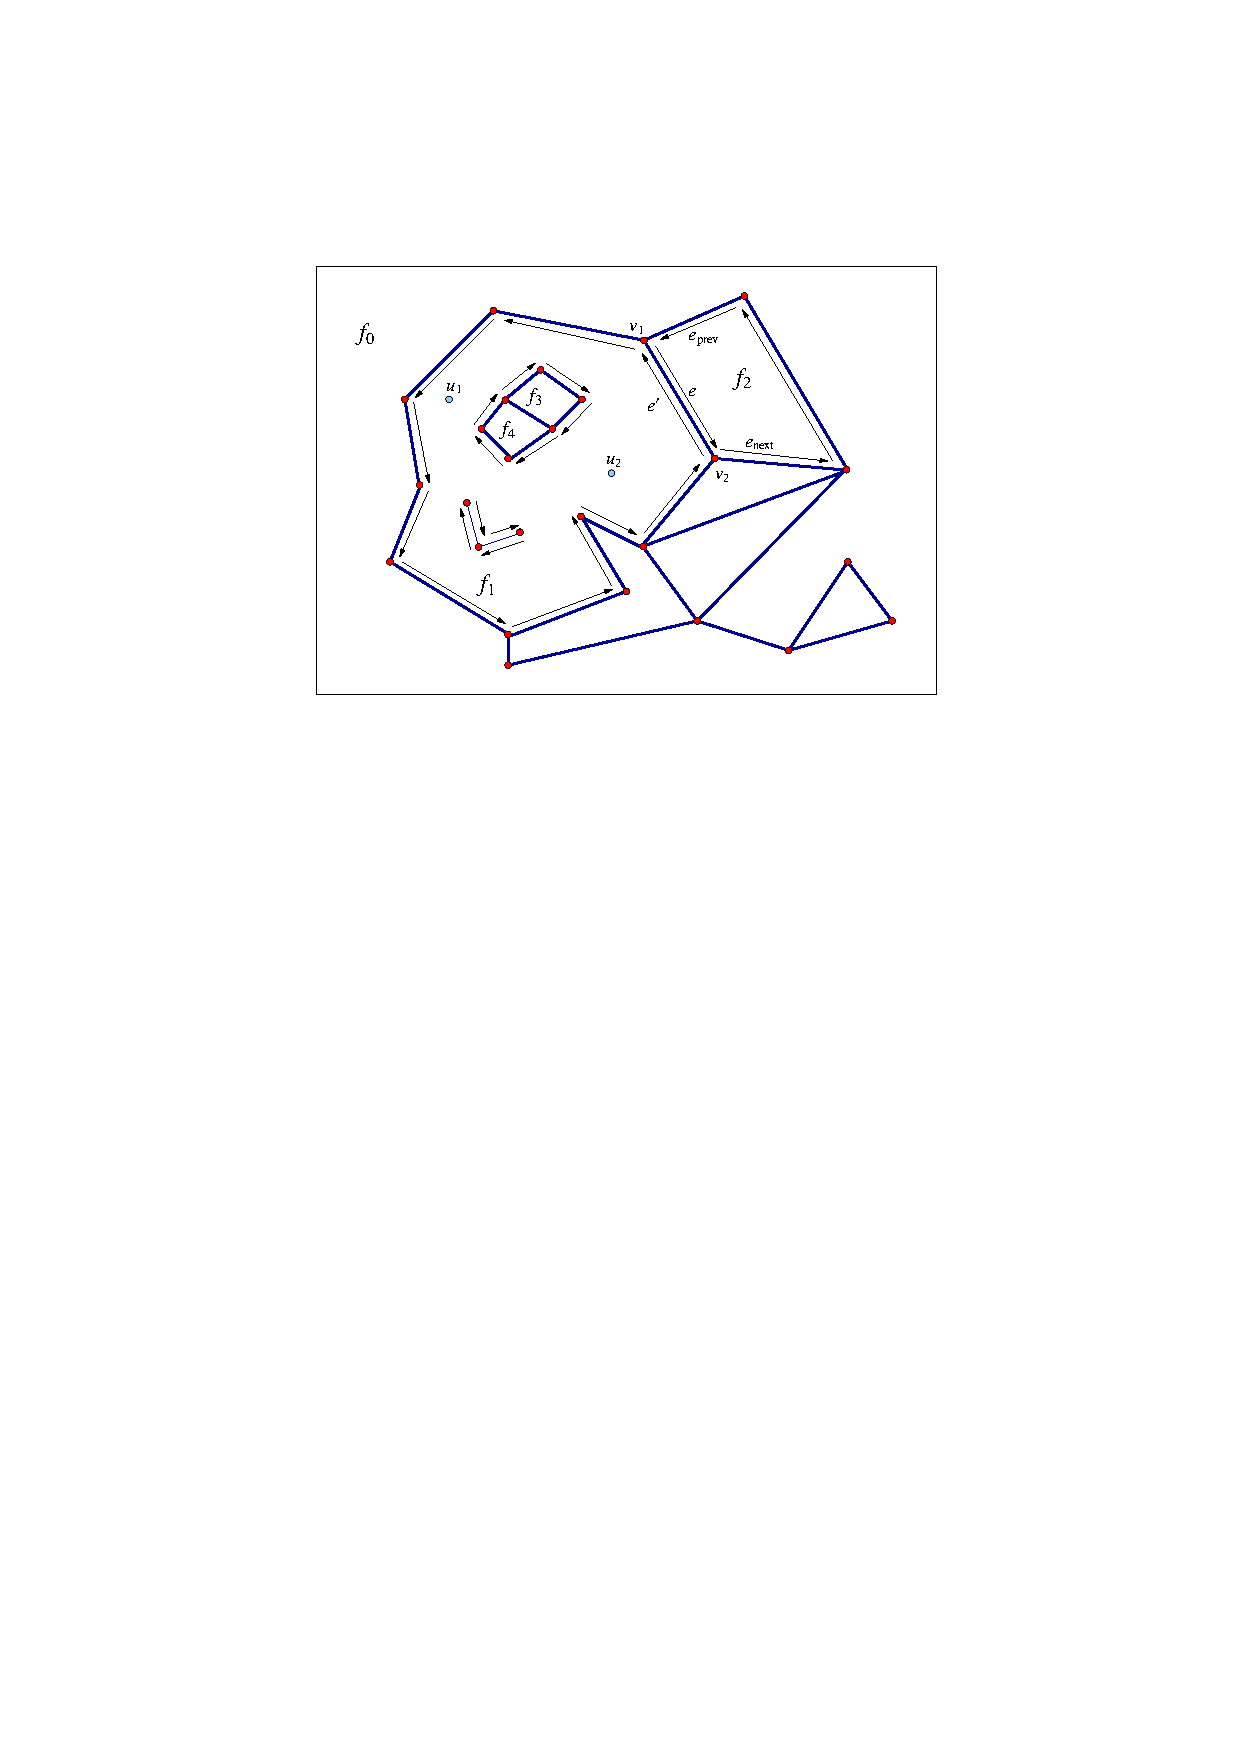
\includegraphics{Arrangement_2/fig/arr_segs}
  \end{center}
\end{ccTexOnly}
\begin{ccHtmlOnly}
  <p><center>
  <img src="./fig/arr_segs.gif" border=0 alt="Arrangement of sgements">
  </center>
\end{ccHtmlOnly}
\caption{An arrangement of interior-disjoint line segments with some
of the \dcel\ records that represent it. The unbounded face $f_0$ has
a single connected component that forms a hole inside it, and this hole
is comprised if several faces. The half-edge $e$ is directed from its
source vertex $v_1$ to its target vertex $v_2$. This edge, together with
its twin $e'$, correspond to a line segment that connects the points
associated with $v_1$ and $v_2$ and separates the face $f_1$ from $f_2$.
The predecessor $e_{\rm prev}$ and successor
$e_{\rm next}$ of $e$ are part of the chain that form the outer
boundary of the face $f_2$. The face $f_1$ has a more complicated
structure as it contains two holes in its interior: One hole
consists of two adjacent faces $f_3$ and $f_4$, while the other
hole is comprised of two edges. $f_1$ also contains two isolated
vertices $u_1$ and $u_2$ in its interior.}
\label{arr_fig:seg_dcel}
\end{figure}

\begin{ccHtmlOnly}<p>\end{ccHtmlOnly}
The rest of this chapter is organized as follows: In
Section~\ref{arr_sec:arr_class} we review in detail the interface
of the \ccc{Arrangement_2} class-template, which is the central
component in the arrangement package. In
Section~\ref{arr_sec:queries} we show how queries on an arrangement
can be issued. In Section~\ref{arr_sec:gl_funcs} we
review some important free (global) functions that operate on
arrangements, the most important ones being the free 
insertion-functions. Section~\ref{arr_sec:traits} contains detailed
descriptions of the various geometric traits classes included in
the arrangement package. Using these traits classes it is possible
to construct arrangements of different families of curves. In
Section~\ref{arr_sec:notif} we review the notification mechanism
that allows external classes to keep track of the changes that an
arrangement instance goes through. Section~\ref{arr_sec:ex_dcel}
explains how to extend the \dcel\ records, to store extra data
with them, and to efficiently update this data.
In Section~\ref{arr_sec:overlay} we introduce the fundamental
operation of overlaying two arrangements.
Section~\ref{arr_sec:arr_with_hist} describes the
\ccc{Arrangement_with_history_2} class-template that extends the
arrangement by storing additional history records with its curves.
Finally, in Section~\ref{arr_sec:io} we review the arrangement
input/output functions.

\section{The Main Arrangement Class}
\label{arr_sec:arr_class}
%===================================
%
The class \ccc{Arrangement_2<Traits,Dcel>} is the main class in
the arrangement package. It is used to represent planar
arrangements and provides the interface needed to construct them,
traverse them, and maintain them. An arrangement is defined by
a geometric {\em traits} class that determines the family of planar
curves that form the arrangement, and a \dcel\ class, which
represents the {\em topological structure} of the planar subdivision.
It supplies a minimal set of geometric operations (predicates and
constructions) required to construct and maintain the arrangement
and to operate on it.

\begin{ccHtmlOnly}<p>\end{ccHtmlOnly}
The design of the arrangement package is guided by the need to
separate between the representation of the arrangements and the
various geometric algorithms that operate on them, and by the need to
separate between the topological and geometric aspects of the planar
subdivision. The separation is exhibited by the two template
parameters of the \ccc{Arrangement_2} template:
\begin{itemize}
\item The \ccc{Traits} template-parameter should be instantiated with
a model of the \ccc{ArrangementBasicTraits_2} concept. The traits
class defines the types of $x$-monotone curves and two-dimensional
points, \ccc{X_monotone_curve_2} and \ccc{Point_2} respectively, and
supports basic geometric predicates on them.

\begin{ccHtmlOnly}<p>\end{ccHtmlOnly}
In the first sections of this chapter we always use
\ccc{Arr_segment_traits_2} as our traits class, to construct
arrangements of line segments. However, the arrangement package 
contains several other traits classes that can handle also
polylines (continuous piecewise-linear curves), conic arcs, and arcs
of rational functions. We exemplify the usage of these traits classes
in Section~\ref{arr_sec:traits}.
\item The \ccc{Dcel} template-parameter should be instantiated with
a class that is a model of the \ccc{ArrangementDcel} concept. The
value of this parameter is \ccc{Arr_default_dcel<Traits>} by default.
However, in many applications it is necessary
to extend the \dcel\ features; see Section~\ref{arr_sec:ex_dcel} for
further explanations and examples.
\end{itemize}

\subsection{A Simple Program}
%----------------------------

\begin{ccHtmlOnly}<p>\end{ccHtmlOnly}
\begin{wrapfigure}[5]{r}{2.5cm}
\vspace{-2.8ex}
  \input{Arrangement_2/fig/triangle.pstex_t}
\vspace{-1.8ex}
\end{wrapfigure}
%
The simple program listed below constructs a planar map of three line
segments forming a triangle. The constructed arrangement is instantiated
with the \ccc{Arr_segment_traits_2} traits class to handle segments only.
The resulting arrangement consists of two faces, a bounded triangular face
and the unbounded face.
The program is not very useful as it is, since it ends immediately
after the arrangement is constructed. We give more enhanced examples
in the rest of this chapter.

\begin{alltt}
#include <CGAL/Cartesian.h>
#include <CGAL/MP_Float.h>
#include <CGAL/Quotient.h>
#include <CGAL/Arr_segment_traits_2.h>
#include <CGAL/Arrangement_2.h>

typedef CGAL::Quotient<CGAL::MP_Float>     Number_type;
typedef CGAL::Cartesian<Number_type>       Kernel;
typedef CGAL::Arr_segment_traits_2<Kernel> Traits;
typedef Traits::Point_2                    Point_2;
typedef Traits::X_monotone_curve_2         X_monotone_curve_2;
typedef CGAL::Arrangement_2<Traits,>       Arrangement_2;

int main()
\{
  Arrangement_2       arr;
  X_monotone_curve_2  cv[3];
  Point_2             p1 (0, 0), p2 (0, 4), p3 (4, 0);
 
  cv[0] = X_monotone_curve_2 (p1, p2);
  cv[1] = X_monotone_curve_2 (p2, p3);
  cv[2] = X_monotone_curve_2 (p3, p1);
  insert(arr, &cv[0], &cv[3]);

  return (0);
\}
\end{alltt}

\subsection{Traversing the Arrangement}
\label{arr_ssec:traverse}
%--------------------------------------
%
The simplest and most fundamental arrangement operations are the
various traversal methods, which allow users to systematically go
over the relevant features of the arrangement at hand.

\begin{ccHtmlOnly}<p>\end{ccHtmlOnly}
As mentioned above, the arrangement is represented as a \dcel,
which stores three containers of vertices, halfedges and faces. Thus,
the \ccc{Arrangement_2} class supplies iterators for these
containers. For example, the methods \ccc{vertices_begin()} and
\ccc{vertices_end()} return \ccc{Arrangement_2::Vertex_iterator}
objects that define the valid range of arrangement vertices. The value
type of this iterator is \ccc{Arrangement_2::Vertex}. Moreover, the
vertex-iterator type is equivalent to
\ccc{Arrangement_2::Vertex_handle}, which serves as a pointer to a
vertex. As we show next, all functions related to arrangement features
accept handle types as input parameters and return handle types as
their output.

\begin{ccHtmlOnly}<p>\end{ccHtmlOnly}
In addition to the iterators for arrangement vertices, halfedges
and faces, the arrangement class also provides \ccc{edges_begin()}
and \ccc{edges_end()} that return
\ccc{Arrangement_2::Edge_iterator} objects for traversing the
arrangement edges. Note that the value type of this iterator is
\ccc{Arrangement_2::Halfedge}, representing one of the twin
halfedges that represent the edge.

\begin{ccHtmlOnly}<p>\end{ccHtmlOnly}
All iterator, circulator\footnote{A {\em circulator} is used to
traverse a circular list, such as the list of halfedges incident to
a vertex --- see below.} and handle types also have non-mutable
({\em const}) counterparts. These non-mutable iterators are useful
to traverse an arrangement without changing it. For example,
the arrangement has a
non-constant member function called \ccc{vertices_begin()} that
returns a \ccc{Vertex_iterator} object and another const member
function that returns a \ccc{Vertex_const_iterator} object. In fact,
all methods listed in this section that return an iterator, a
circulator or a handle have non-mutable counterparts. It should be
noted that, for example, \ccc{Vertex_handle} can be readily converted
into a \ccc{Vertex_const_handle}, but not vice-versa.

\begin{ccHtmlOnly}<p>\end{ccHtmlOnly}
Conversion of a non-mutable handle to a corresponding mutable
handle are nevertheless possible, and can be performed using the
static function \ccc{Arrangement_2::non_const_handle()} (see, e.g.,
Section~\ref{arr_ssec:pl}). There are
three variant of this function, one for each type of handle.

\subsubsection{Traversal Methods for an Arrangement Vertex}
\label{arr_sssec:tr_vertex}
%~~~~~~~~~~~~~~~~~~~~~~~~~~~~~~~~~~~~~~~~~~~~~~~~~~~~~~~~~~
%
A vertex is always associated with a geometric entity, namely with
a \ccc{Point_2} object, which can be obtained by the \ccc{point()}
method of the \ccc{Vertex} class nested within \ccc{Arrangement_2}.

\begin{ccHtmlOnly}<p>\end{ccHtmlOnly}
The \ccc{is_isolated()} method determines whether a vertex is isolated
or not. Recall that the halfedges incident to a non-isolated vertex,
namely the halfedges that share a common target vertex, form a circular
list around this vertex. The \ccc{incident_halfedges()} method returns
a circulator of type \ccc{Arrangement_2::Halfedge_around_vertex_circulator}
that enables the traversal of this circular list in a clockwise
direction. The value type of this circulator is \ccc{Halfedge}.

\begin{ccHtmlOnly}<p>\end{ccHtmlOnly}
The following function prints all the neighbors of a given
arrangement vertex (assuming that the \ccc{Point_2} type can be
inserted into the standard output using the \ccc{<<} operator). The
arrangement type is the same as in the simple example above.
\begin{alltt}
void print_neighboring_vertices (Arrangement_2::Vertex_const_handle v)
\{
  if (v->is_isolated()) \{
    std::cout << "The vertex (" << v->point() << ") is isolated" << std::endl;
    return;
  \}

  Arrangement_2::Halfedge_around_vertex_const_circulator first, curr;
  first = curr = v->incident_halfedges();

  std::cout << "The neighbors of the vertex (" << v->point() << ") are:";
  do \{
    // Note that the current halfedge is directed from u to v:
    Arrangement_2::Vertex_const_handle u = curr->source();
    std::cout << " (" << u->point() << ")";
  \} while (++curr != first);
  std::cout << std::endl;
\}
\end{alltt}

\begin{ccHtmlOnly}<p>\end{ccHtmlOnly}
In case of an isolated vertex, it is possible to obtain the face
that contains this vertex using the \ccc{face()} method.

\subsubsection{Traversal Methods for an Arrangement Halfedge}
\label{arr_sssec:tr_halfedge}
%~~~~~~~~~~~~~~~~~~~~~~~~~~~~~~~~~~~~~~~~~~~~~~~~~~~~~~~~~~~~
%
Each arrangement edge, realized as a pair of twin halfedges,
is associated with an \ccc{X_monotone_curve_2} object, which
can be obtained by the \ccc{curve()} method of the \ccc{Halfedge}
class nested in the \ccc{Arrangement_2} class.

\begin{ccHtmlOnly}<p>\end{ccHtmlOnly}
The \ccc{source()} and \ccc{target()} methods return handles to
the halfedge source and target vertices respectively. We can
obtain a handle to the twin halfedge using the \ccc{twin()}
method. From the definition of halfedges, it follows that if
\ccc{he} is a halfedge handle, then:
\begin{itemize}
\item \ccc{he->curve()} is equivalent to \ccc{he->twin()->curve()},
\item \ccc{he->source()} is equivalent to \ccc{he->twin()->target()}, and
\item \ccc{he->target()} is equivalent to \ccc{he->twin()->source()}.
\end{itemize}

\begin{ccHtmlOnly}<p>\end{ccHtmlOnly}
Every halfedge has an incident face that lies to its left, which
can be obtained by the \ccc{face()} method. Recall that a
halfedge is always one link in a connected chain of halfedges that
share the same incident face, known as a {\em CCB}. The
\ccc{prev()} and \ccc{next()} methods return handles to the
previous and next halfedges in the CCB respectively. 
%(note that \ccc{he->prev()} is not necessarily equivalent to
%\ccc{he->twin()->next()}).

\begin{ccHtmlOnly}<p>\end{ccHtmlOnly}
As the CCB is a circular list of halfedges, it is only natural to 
traverse it using a circulator. The \ccc{ccb()} method returns a 
\ccc{Arrangement_2::Ccb_halfedge_circulator} object for the
halfedges along the CCB.

\begin{ccHtmlOnly}<p>\end{ccHtmlOnly}
The function \ccc{print_ccb()} listed below prints all $x$-monotone
curves along a given CCB (assuming that the \ccc{Point_2} and the
\ccc{X_monotone_curve_2} types can be inserted into the standard output
using the \ccc{<<} operator).
\begin{alltt}
void print_ccb (Arrangement_2::Ccb_halfedge_const_circulator circ)
\{
  Ccb_halfedge_const_circulator curr = circ;
  std::cout << "(" << curr->source()->point() << ")";
  do \{
    Arrangement_2::Halfedge_const_handle he = curr->handle();
    std::cout << "   [" << he->curve() << "]   "
              << "(" << he->target()->point() << ")";
  \} while (++curr != circ);
  std::cout << std::endl;
\}
\end{alltt}

\subsubsection{Traversal Methods for an Arrangement Face}
\label{arr_sssec:tr_face}
%~~~~~~~~~~~~~~~~~~~~~~~~~~~~~~~~~~~~~~~~~~~~~~~~~~~~~~~~
%
An arrangement of bounded curves always has a single unbounded face.
The function \ccc{unbounded_face()} returns a handle to this face.
(Note that an empty arrangement contains nothing {\em but} the
unbounded face.)

\begin{ccHtmlOnly}<p>\end{ccHtmlOnly}
Given a \ccc{Face} object, we can use the \ccc{is_unbounded()}
method to determine whether it is unbounded. Bounded faces have an
outer CCB, and the \ccc{outer_ccb()} method returns a circulator
for the halfedges along this CCB. Note that the halfedges along
this CCB wind in a counterclockwise orientation around the outer
boundary of the face.

\begin{ccHtmlOnly}<p>\end{ccHtmlOnly}
A face can also contain disconnected components in its interior,
namely holes and isolated vertices:
\begin{itemize}
\item The \ccc{holes_begin()} and \ccc{holes_end()} methods return
\ccc{Arrangement_2::Holes_iterator} iterators that define the range
of holes inside the face. The value type of this iterator is
\ccc{Ccb_halfedge_circulator}, defining the CCB that winds in a
clockwise orientation around a hole.
\item The \ccc{isolated_vertices_begin()} and
\ccc{isolated_vertices_end()} methods return
\ccc{Arrangement_2::Isolated_vertices_iterator} iterators that
define the range of isolated vertices inside the face. The value
type of this iterator is \ccc{Vertex}.
\end{itemize}

\begin{ccHtmlOnly}<p>\end{ccHtmlOnly}
The function \ccc{print_face()} listed below prints the outer and
inner boundaries of a given face, using the function \ccc{print_ccb()},
which was introduced in the previous subsection.
\begin{alltt}
void print_face (Arrangement_2::Face_const_handle f)
\{
  // Print the outer boundary.
  if (f->is_unbounded())
    std::cout << "Unbounded face. " << std::endl;
  else \{
    std::cout << "Outer boundary: ";
    print_ccb (f->outer_ccb());
  \}

  // Print the boundary of each of the holes.
  Arrangement_2::Holes_const_iterator hi;
  int                                 index = 1;
  for (hi = f->holes_begin(); hi != f->holes_end(); ++hi, ++index) \{
    std::cout << "    Hole #" << index << ": ";
    print_ccb (*hi);
  \}

  // Print the isolated vertices.
  Arrangement_2::Isolated_vertices_const_iterator iv;
  for (iv = f->isolated_vertices_begin(), index = 1;
       iv != f->isolated_vertices_end(); ++iv, ++index)
  \{
    std::cout << "    Isolated vertex #" << index << ": "
              << "(" << iv->point() << ")" << std::endl;
  \}
\}
\end{alltt}

\subsubsection{Additional Example}
\label{arr_sssec:tr_ex}
%~~~~~~~~~~~~~~~~~~~~~~~~~~~~~~~~~
%
The function listed below prints the current setting of a given
arrangement. This concludes the preview of the various traversal
methods.\footnote{The file \ccc{arr_print.h}, which can be
found under the examples folder, includes this function and the
rest of the functions listed in this section. Over there they are
written in a more generic fashion, where the arrangement type
serves as a template parameter for these functions, so different
instantiations of the \ccc{Arrangement_2<Traits,Dcel>} template
can be provided to the same function templates.}
\begin{alltt}
void print_arrangement (const Arrangement_2& arr)
\{
  // Print the arrangement vertices.
  Vertex_const_iterator vit;
  std::cout << arr.number_of_vertices() << " vertices:" << std::endl;
  for (vit = arr.vertices_begin(); vit != arr.vertices_end(); ++vit) \{
    std::cout << "(" << vit->point() << ")";
    if (vit->is_isolated())
      std::cout << " - Isolated." << std::endl;
    else
      std::cout << " - degree " << vit->degree() << std::endl;
  \}

  // Print the arrangement edges.
  Edge_const_iterator eit;
  std::cout << arr.number_of_edges() << " edges:" << std::endl;
  for (eit = arr.edges_begin(); eit != arr.edges_end(); ++eit)
    std::cout << "[" << eit->curve() << "]" << std::endl;

  // Print the arrangement faces.
  Face_const_iterator fit;
  std::cout << arr.number_of_faces() << " faces:" << std::endl;
  for (fit = arr.faces_begin(); fit != arr.faces_end(); ++fit)
    print_face (fit);
\}
\end{alltt}

\subsection{Modifying the Arrangement}
\label{arr_ssec:modify}
%-------------------------------------
%
In this section we review the various member functions of the
\ccc{Arrangement_2} class that allow users to modify the
topological structure of the arrangement by introducing new edges
or vertices, modifying them, or removing them.

\begin{ccHtmlOnly}<p>\end{ccHtmlOnly}
The arrangement member-functions that insert new curves into the
arrangement, thus enabling the construction of a planar subdivision, are
rather specialized, as they require a-priori knowledge on the location of
the inserted curve. Indeed, for most purposes it is more convenient to
construct an arrangement using the free (global) insertion-functions.

\subsubsection{Inserting Non-Intersecting $x$-Monotone Curves}
\label{arr_sssec:mf_insert_cv}
%~~~~~~~~~~~~~~~~~~~~~~~~~~~~~~~~~~~~~~~~~~~~~~~~~~~~~~~~~~~~~
%
The most important functions that allow users to modify the
arrangement, and perhaps the most frequently used ones, are the
specialized insertion functions of $x$-monotone curves whose
interior is disjoint from any other curve in the existing
arrangement and do not contain any vertex of the arrangement. In
addition, these function require that the location of the curve in the
arrangement is known.

\begin{ccHtmlOnly}<p>\end{ccHtmlOnly}
The motivation behind these rather harsh restrictions on the nature of
the inserted curves is the decoupling of the topological arrangement
representation from the various algorithms that operate on it. While
the insertion of an $x$-monotone curve whose interior is disjoint from
all existing arrangement features is quite straightforward (as we show
next), inserting curves that intersect with the curves already inserted
into the arrangement is much more complicated and requires the
application of non-trivial geometric algorithms.
These insertion operations are therefore implemented as free functions
that operate on the arrangement and the inserted curve(s); see
Section~\ref{arr_sec:gl_funcs} for more details and
examples.\footnote{You may skip to Section~\ref{arr_sec:gl_funcs},
and return to this subsection at a later point in time.}

\begin{figure}[!htp]
\begin{ccTexOnly}
  \begin{center}
  \begin{tabular}{ccc}
    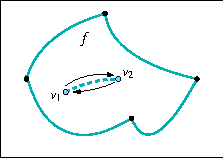
\includegraphics{Arrangement_2/fig/insert_in_face} &
    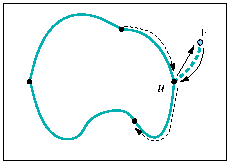
\includegraphics{Arrangement_2/fig/insert_from_vertex} &
    
\includegraphics{Arrangement_2/fig/insert_at_vertices}\\
  {\small (a)} & {\small (b)} & {\small (c)}\\
  \end{tabular}
  \end{center}
\end{ccTexOnly}
\begin{ccHtmlOnly}
  <p><center>
    <img src="./fig/insert.gif" border=0 alt="insert">
  </center>
\end{ccHtmlOnly}
\caption{The various specialized insertion procedures. The
inserted $x$-monotone curve is drawn with a light dashed line,
surrounded by two solid arrows that represent the pair of twin
half-edges added to the \dcel. Existing vertices are shown as
black dots while new vertices are shown as light dots. Existing
half-edges that are affected by the insertion operations are drawn
as dashed arrows. (a) Inserting a curve as a new hole inside the
face $f$. (b) Inserting a curve from an existing vertex $u$ that
corresponds to one of its endpoints. (c) Inserting an $x$-monotone
curve whose endpoints are the already existing vertices
$u_1$ and $u_2$. In our case, the new pair of half-edges close a
new face $f'$, where the hole $h_1$, which used to belong to $f$,
now becomes an enclave in this new face.} \label{arr_fig:insert}
\end{figure}

\begin{ccHtmlOnly}<p>\end{ccHtmlOnly}
When an $x$-monotone curve is inserted into an existing arrangement, such
that the interior of this curve is disjoint from any arrangement feature,
only the following three scenarios are possible, depending on the status
of the endpoints of the inserted subcurve:
\begin{enumerate}
%
\item In case both curve endpoints do not correspond to any existing
arrangement vertex we have to create two new vertices
corresponding to the curve endpoints and connect them using a pair
of twin halfedges. This halfedge pair initiates a new hole inside
the face that contains the curve in its interior.
%
\item If exactly one endpoint corresponds to an existing arrangement
vertex (we distinguish between a vertex that corresponds to the left
endpoint of the inserted curve and a vertex corresponding to its right
endpoint), we have to create a new vertex that corresponds to the other
endpoint of the curve and to connect the two vertices by a pair of
twin halfedges that form an ``antenna'' emanating from the boundary
of an existing connected component (note that if the existing vertex
used to be isolated, this operation is actually equivalent to forming
a new hole inside the face that contains this vertex).
\end{enumerate}

\begin{wrapfigure}{r}{4.5cm}
\vspace{-1.2ex}
  \input{Arrangement_2/fig/connect_comp.pstex_t}
\vspace{-1.8ex}
\end{wrapfigure}
%
~~~~
\vspace{-8ex}
\begin{enumerate}
\item[3.] If both endpoints correspond to existing arrangement
vertices, we connect these vertices using a pair of twin halfedges.
(If one or both vertices are isolated this case reduces to one of
the two previous cases respectively.) The two following subcases may
occur:
\begin{itemize}
\item Two disconnected components are merged into a single connected
component (as is the case with the segment $s_1$ in the figure to the
left).
%
\item A new face is created, a face that splits from an existing
arrangement face. In this case we also have to examine the holes and
isolated vertices in the existing face and move the relevant ones
inside the new face (as is the case with the segment $s_2$ in the
figure to the left).
\end{itemize}
\end{enumerate}

\begin{ccHtmlOnly}<p>\end{ccHtmlOnly}
The \ccc{Arrangement_2} class offers insertion functions named
\ccc{insert_in_face_interior()}, \ccc{insert_from_left_vertex()},
\ccc{insert_from_right_vertex()} and \ccc{insert_at_vertices()}
that perform the special insertion procedures listed above. The
first function accepts an $x$-monotone curve $c$ and an arrangement
face $f$ that contains this curve in its interior. The other
functions accept an $x$-monotone curve $c$ and handles to the existing
vertices that correspond to the curve endpoint(s). Each of the four
functions returns a handle to one of the twin halfedges that have
been created, where:
\begin{itemize}
\item \ccc{insert_in_face_interior(c, f)} returns a halfedge directed
from the vertex corresponding to the left endpoint of \ccc{c}
toward the vertex corresponding to its right endpoint.
%
\item \ccc{insert_from_left_vertex(c, v)} and
\ccc{insert_from_right_vertex(c, v)} returns a halfedge whose
source is the vertex $v$ that and whose target is the new vertex
that has just been created.
%
\item \ccc{insert_at_vertices(c, v1, v2)} returns a halfedge directed
from $v_1$ to $v_2$.
\end{itemize}

\begin{figure}[!htp]
\begin{ccTexOnly}
  \begin{center}
  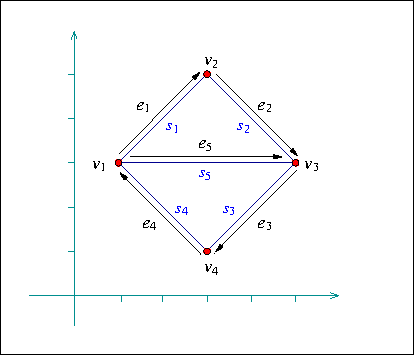
\includegraphics{Arrangement_2/fig/ex_1}
  \end{center}
\end{ccTexOnly}
\begin{ccHtmlOnly}
  <p><center>
  <img src="./fig/ex_1.gif" border=0 alt="Example 1">
  </center>
\end{ccHtmlOnly}
\caption{The arrangement of the line segments $s_1, \ldots, s_5$
constructed in \ccc{ex_edge_insertion.C}. The arrows mark the direction of
the halfedges returned from the various insertion functions.}
\label{arr_fig:ex_1}
\end{figure}

\begin{ccHtmlOnly}<p>\end{ccHtmlOnly}
The following program demonstrates the usage of the four insertion
functions. It creates an arrangement of five line segments, as
depicted in Figure~\ref{arr_fig:ex_1}.\footnote{Notice that in all
figures in the rest of this chapter the coordinate axes are drawn
only for illustrative purposes and are {\em not} part of the
arrangement.} As the arrangement is very
simple, we use the simple Cartesian kernel of \cgal\ with integer
coordinates for the segment endpoints. We also use the 
\ccc{Arr_segment_traits_2} class that enables the efficient
maintenance of arrangements of line segments; see more details on
this traits class in Section~\ref{arr_sec:traits}. This example, as
many others in this chapter, uses some print-utility functions from
the file \ccc{print_arr.h}; these functions are also listed in
Section~\ref{arr_ssec:traverse}.

\ccIncludeExampleCode{../examples/Arrangement_2/ex_edge_insertion.C}

\begin{ccHtmlOnly}<p>\end{ccHtmlOnly}
Observe that the first line segment is inserted in the interior of
the unbounded face. The other line segments are inserted
using the vertices created by the insertion of previous segments.
The resulting arrangement consists of three faces, where the two
bounded faces form together a hole in the unbounded face.

\subsubsection{Manipulating Isolated Vertices}
\label{arr_sssec:mf_iso_verts}
%~~~~~~~~~~~~~~~~~~~~~~~~~~~~~~~~~~~~~~~~~~~~~~~~
%
Isolated points are in general simpler geometric entities than
curves and indeed the member functions that manipulate them are
easier to understand.

\begin{ccHtmlOnly}<p>\end{ccHtmlOnly}
The function \ccc{insert_in_face_interior(p, f)} inserts an
isolated point $p$, located in the interior of a given face $f$,
into the arrangement and returns a handle to the arrangement
vertex it has created and associated with $p$. Naturally, this
function has a precondition that $p$ is really an isolated point,
namely it does not coincide with any existing arrangement vertex
and does not lie on any edge. As mentioned in
Section~\ref{arr_ssec:traverse}, it is possible to obtain the face
containing an isolated vertex handle $v$ by calling \ccc{v->face()}.

\begin{ccHtmlOnly}<p>\end{ccHtmlOnly}
The function \ccc{remove_isolated_vertex(v)} receives a handle to
an isolated vertex and removes it from the arrangement.

\begin{figure}[!htp]
\begin{ccTexOnly}
  \begin{center}
  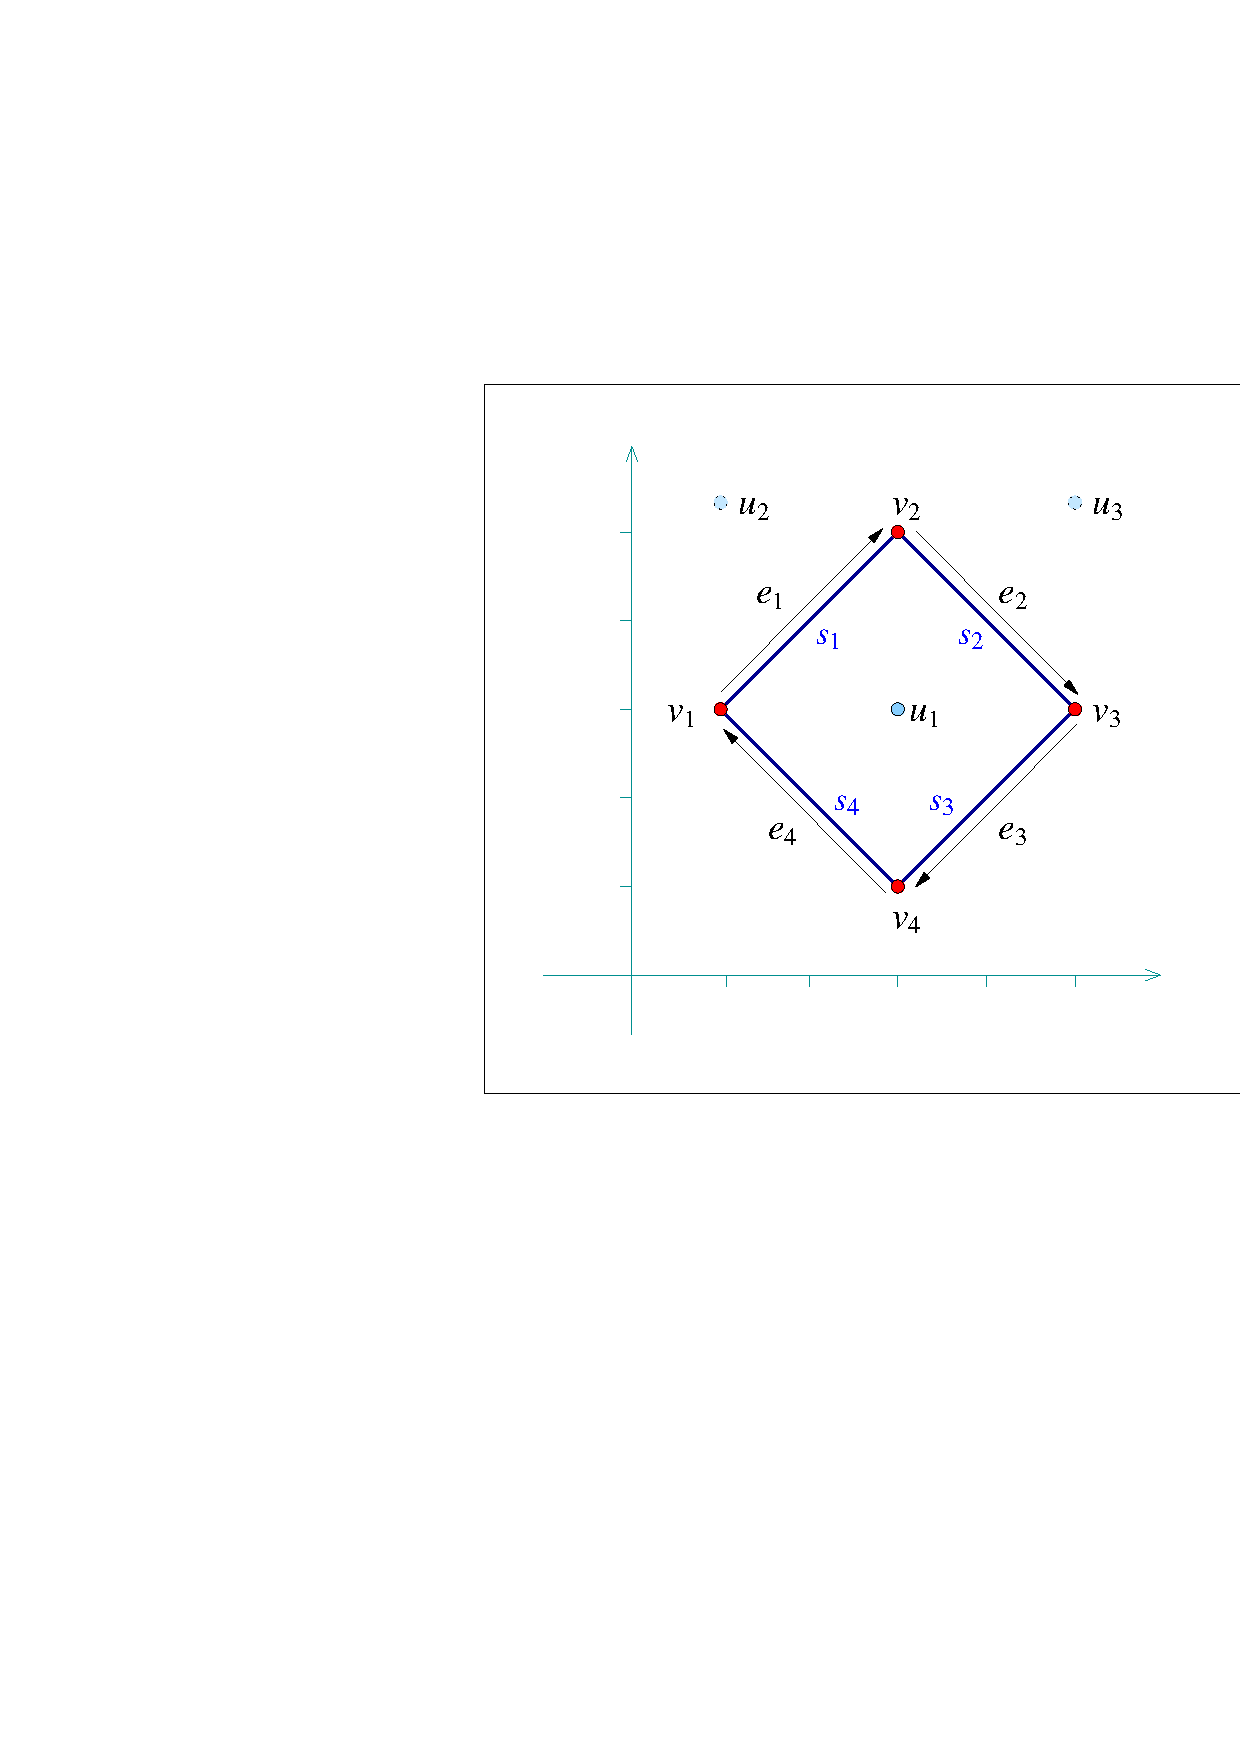
\includegraphics{Arrangement_2/fig/ex_2}
  \end{center}
\end{ccTexOnly}
\begin{ccHtmlOnly}
  <p><center>
  <img src="./fig/ex_2.gif" border=0 alt="Example 2">
  </center>
\end{ccHtmlOnly}
\caption{An arrangement of line segments containing three isolated
vertices, as constructed in \ccc{ex_isolated_vertices.C}. The vertices $u_2$
and $u_3$ are eventually removed from the arrangement.}
\label{arr_fig:ex_2}
\end{figure}

\begin{ccHtmlOnly}<p>\end{ccHtmlOnly}
The following program demonstrates the usage of the arrangement
member-functions for manipulating isolated vertices. It first
inserts three isolated vertices located inside the unbounded face, then
it inserts four line segments that form a rectangular hole inside the
unbounded face (see Figure~\ref{arr_fig:ex_2} for an
illustration). Finally, it traverses the vertices and removes those
isolated vertices that are still contained in the unbounded face
($u_2$ and $u_3$ in this case):

\ccIncludeExampleCode{../examples/Arrangement_2/ex_isolated_vertices.C}

\subsubsection{Manipulating Halfedges}
\label{arr_sssec:mf_halfedges}
%~~~~~~~~~~~~~~~~~~~~~~~~~~~~~~~~~~~~~~~~~~~~~~~~
%
In the previous subsection we showed how to introduce new isolated
vertices in the arrangement. But how does one create a vertex that
lies on an existing arrangement edge (more precisely, on an
$x$-monotone curve that is associated with an arrangement edge)?

\begin{ccHtmlOnly}<p>\end{ccHtmlOnly}
It should be noted that such an operation involves the splitting
of a curve at a given point in its interior, while the traits
class used by \ccc{Arrangement_2} does not necessarily have the
ability to perform such a split operation. However, if users have
the ability to split an $x$-monotone curve into two at a given point
$p$ (this is usually the case when employing a more sophisticated
traits class; see Section~\ref{arr_sec:traits} for more details)
they can use the \ccc{split_edge(e, c1, c2)} function, were
$c_1$ and $c_2$ are the two subcurves resulting from splitting the
$x$-monotone curve associated with the halfedge $e$ at some point
(call it $p$) in its interior. The function splits the halfedge pair into two
pairs, both incident to a new vertex $v$ associated with $p$, and
returns a handle to a halfedge whose source equals $e$'s source
vertex and whose target is the new vertex $v$.

\begin{ccHtmlOnly}<p>\end{ccHtmlOnly}
The reverse operation is also possible. Suppose that we have a
vertex $v$ of degree $2$, whose two incident halfedges, $e_1$ and
$e_2$, are associated with the curves $c_1$ and $c_2$. Suppose
further that it is possible to merge these two curves into a single
continuous $x$-monotone curve $c$. Calling \ccc{merge_edge(e1, e2, c)}
will merge the two edges into a single edge associated with the curve
$c$, essentially removing the vertex $v$ from the arrangement.

\begin{ccHtmlOnly}<p>\end{ccHtmlOnly}
Finally, the function \ccc{remove_edge(e)} removes the edge $e$
from the arrangement. Note that this operation is the reverse of
an insertion operation, so it may cause a connected
component to split into two, or two faces to merge into one, or a
hole to disappear. By default, if the removal of \ccc{e} causes one
of its end-vertices to become isolated, we remove this vertex as well.
However, users can control this behavior and choose to keep the
isolated vertices by supplying additional Boolean flags to
\ccc{remove_edge()} indicating whether the source and the target vertices
are to be removed should they become isolated.

\begin{figure}[!htp]
\begin{ccTexOnly}
  \begin{center}
  \begin{tabular}{ccc}
    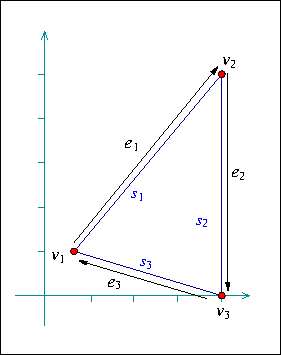
\includegraphics{Arrangement_2/fig/ex_3a} &
    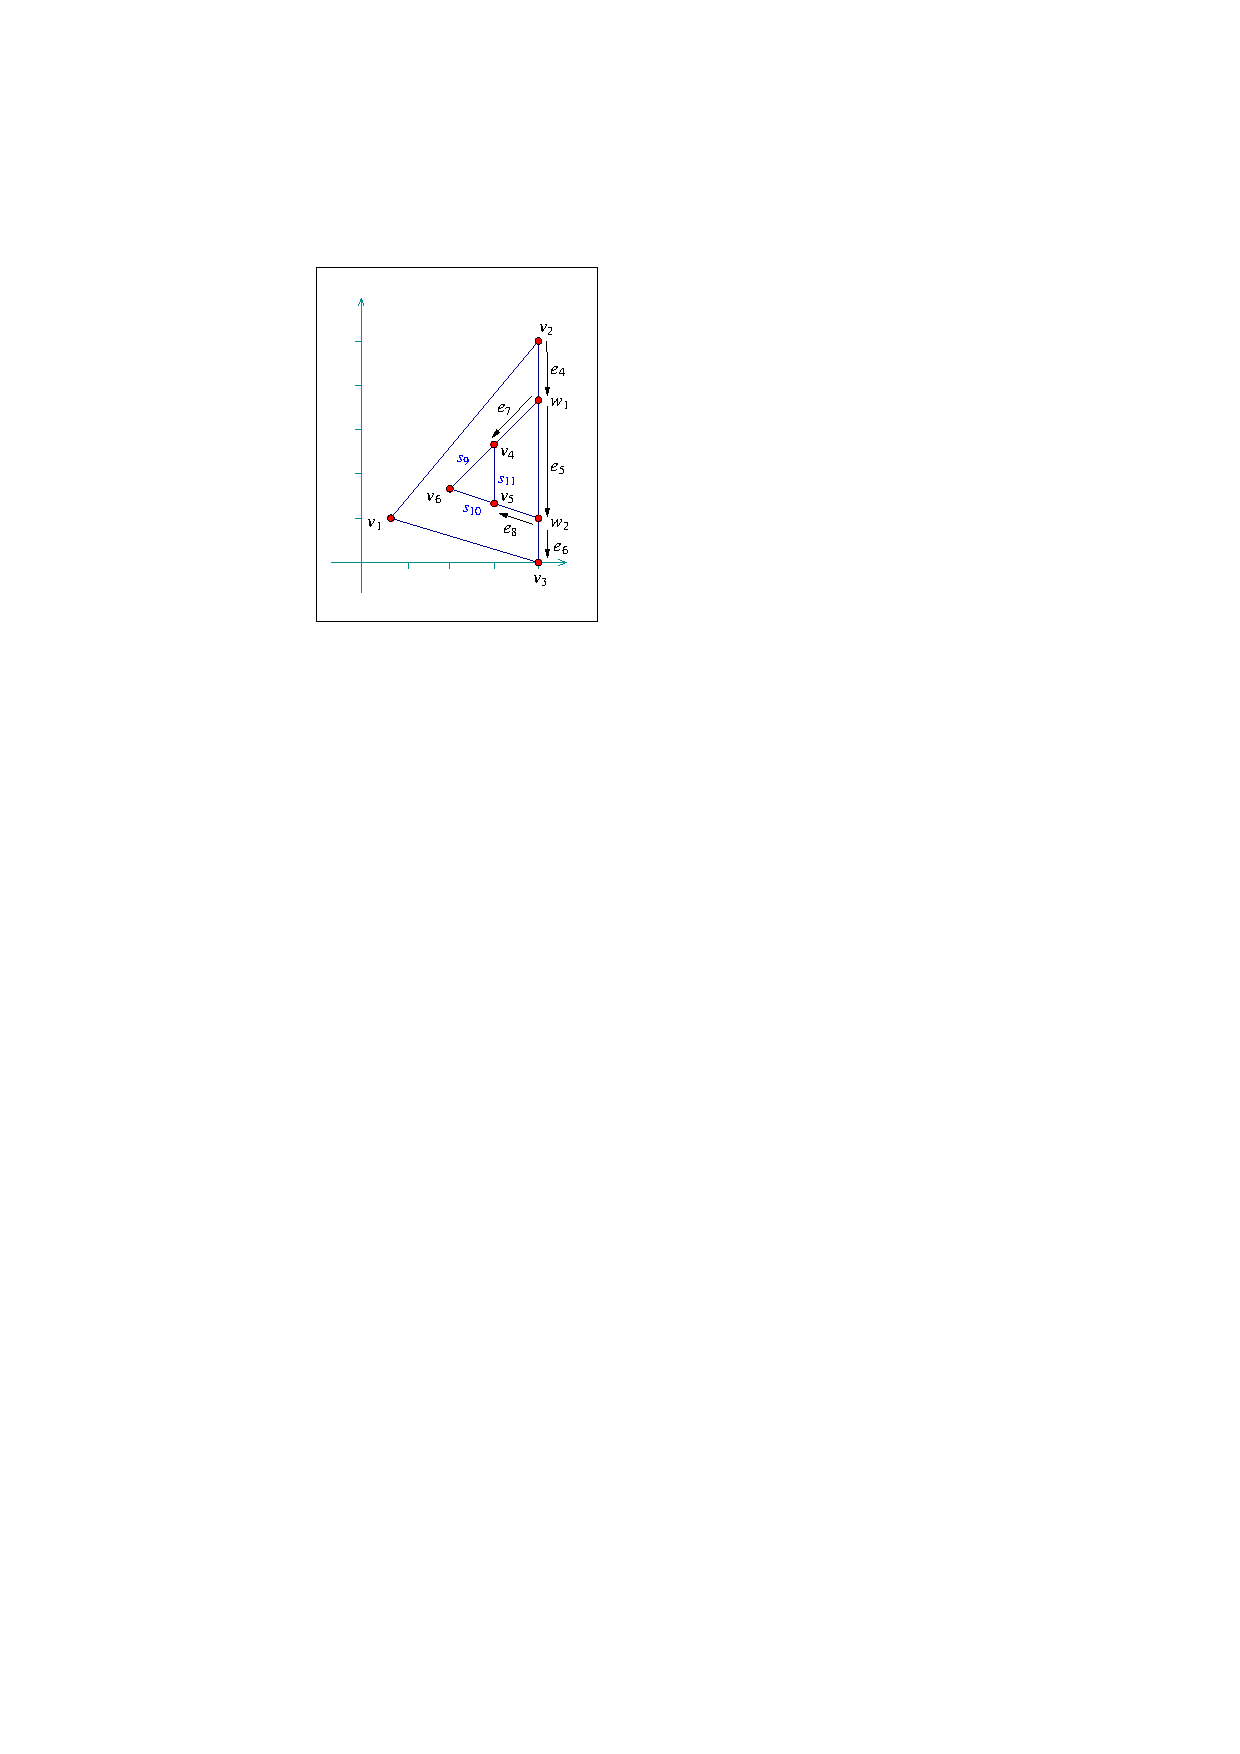
\includegraphics{Arrangement_2/fig/ex_3b} &
    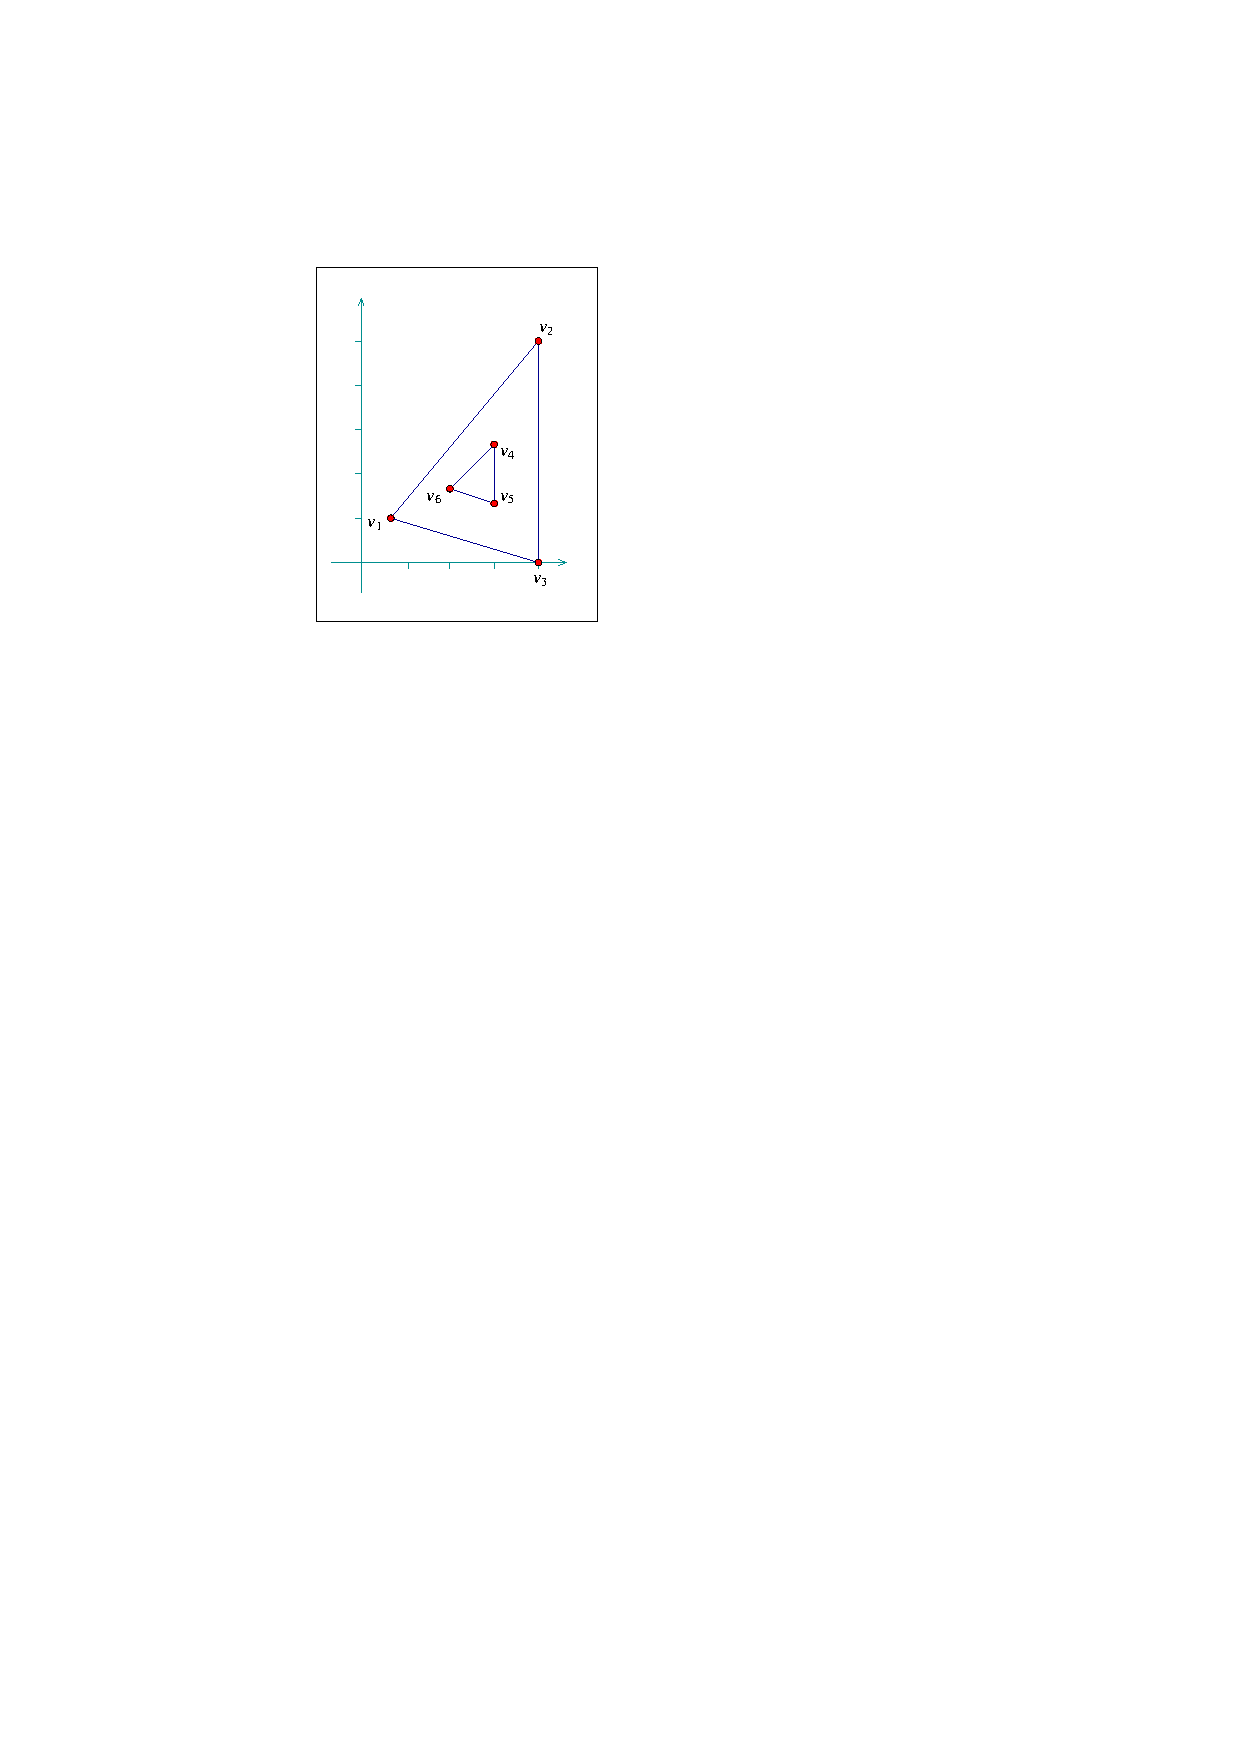
\includegraphics{Arrangement_2/fig/ex_3c} \\
  {\small (a)} & {\small (b)} & {\small (c)}\\
  \end{tabular}
  \end{center}
\end{ccTexOnly}
\begin{ccHtmlOnly}
  <p><center>
  <img src="./fig/ex_3.gif" border=0 alt="Example 3">
  </center>
\end{ccHtmlOnly}
\caption{An arrangement of line segments as constructed
in \ccc{ex_edge_manipulation.C}. Note that the edges $e_7$ and $e_8$ and the
vertices $w_1$ and $w_2$, introduced in step~(b) are eventually
removed in step~(c).}
\label{arr_fig:ex_3}
\end{figure}

\begin{ccHtmlOnly}<p>\end{ccHtmlOnly}
In the following example program we show how the edge-manipulation
functions can be used. The program works in three
steps, as demonstrated in Figure~\ref{arr_fig:ex_3}. Note that
here we still stick to integer coordinates, but as we work on a
larger scale we use an unbounded integer number-type (in this
case, the \ccc{Gmpz} type taken from the {\sc Gmp} library)
instead of the built-in \ccc{int} type.\footnote{As a rule of
thumb, one can use a bounded integer type for representing line
segments whose coordinates are bounded by
$\lfloor\sqrt[3]{M}\rfloor$, where $M$ is the maximal
representable integer value. This guarantees that no overflows occur
in the computations carried out by the traits class, hence all traits-class
predicates always return correct results.} We also use the standard Cartesian
kernel of \cgal\ as our kernel. This is recommended when the
kernel is instantiated with a more complex number type, as we
demonstrate in other examples in this chapter.

\ccIncludeExampleCode{../examples/Arrangement_2/ex_edge_manipulation.C}

\begin{ccHtmlOnly}<p>\end{ccHtmlOnly}
Note how we use the halfedge handles returned from
\ccc{split_edge()} and \ccc{merge_edge()}. Also note the insertion
of the isolated vertex $v_6$ located inside the triangular face (the
incident face of $e_7$). This vertex seizes from being isolated, as it
is gets connected to other vertices.

\begin{ccHtmlOnly}<p>\end{ccHtmlOnly}
In this context, we should mention the two member functions
\ccc{modify_vertex(v, p)}, which sets $p$ to be the point
associated with the vertex $v$, and \ccc{modify_edge(e, c)}, which
sets $c$ to be the $x$-monotone curve associated with the halfedge
$e$. These functions have preconditions that $p$ is
geometrically equivalent to \ccc{v->point()} and $c$ is equivalent
to \ccc{e->curve()} (i.e., the two curves have the same graph),
respectively, to avoid the invalidation of the geometric structure of
the arrangement. At a first glance it may seen as these two functions
are of little use. However, we should keep in mind that there may be
extraneous data (probably non-geometric) associated with the point
objects or with the curve objects, as defined by the traits class. With
these two functions we can modify this data; see more details in
Section~\ref{arr_sec:traits}.

\begin{ccHtmlOnly}<p>\end{ccHtmlOnly}
In addition, we can use these functions to replace a geometric
object (a point or a curve) with an equivalent object that has a
more compact representation. For example, we can replace the point
$(\frac{20}{40}, \frac{99}{33})$ associated with some vertex $v$,
by $(\frac{1}{2}, 3)$.

\begin{ccAdvanced}
\subsubsection{Advanced Insertion Functions}
\label{arr_sssec:adv_insert}
%~~~~~~~~~~~~~~~~~~~~~~~~~~~~~~~~~~~~~~~~~~~
%
\begin{wrapfigure}{r}{4.5cm}
\vspace{-1.2ex}
  \input{Arrangement_2/fig/pred_around_vertex.pstex_t}
\vspace{-1.8ex}
\end{wrapfigure}
%
Assume that the specialized insertion function
\ccc{insert_from_left_vertex(c,v)} is invoked for a curve $c$,
whose left endpoint is already associated with a non-isolated
vertex $v$.  Namely, $v$ has already several incident halfedges. It
is necessary in this case to locate the exact place for the
new halfedge mapped to the inserted new curve $c$ in the circular
list of halfedges incident to $v$. More precisely, it is sufficient
to locate one of the halfedges \ccc{pred} directed toward $v$ such
that $c$ is located between \ccc{pred} and \ccc{pred->next()} in
clockwise order around $v$, in order to complete the insertion
(see Figure~\ref{arr_fig:insert} for an illustration). This may
take $O(d)$ time where $d$ is the degree of the vertex. However,
if the halfedge \ccc{pred} is known in advance, the insertion can
be carried out in constant time.

\begin{ccHtmlOnly}<p>\end{ccHtmlOnly}
The \ccc{Arrangement_2} class provides the advanced versions of
the specialized insertion functions for a curve $c$ --- namely we have
\ccc{insert_from_left_vertex(c,pred)} and
\ccc{insert_from_right_vertex(c,pred)} that accept a halfedge \ccc{pred}
as specified above, instead of a vertex $v$. These functions are
more efficient, as they take constant time and do not perform any
geometric operations. Thus, they should be used when the halfedge
\ccc{pred} is known. In case that the vertex $v$ is isolated or
that the predecessor halfedge for the new inserted curve is not
known, the simpler versions of these insertion functions should be
used.

\begin{ccHtmlOnly}<p>\end{ccHtmlOnly}
Similarly, there exist two overrides of the
\ccc{insert_at_vertices()} function: One that accept the two
predecessor halfedges around the two vertices $v_1$ and $v_2$ that
correspond to the curve endpoints, and one that accepts a handle
for one vertex and a predecessor halfedge around the other
vertex.

\begin{figure}[!htp]
\begin{ccTexOnly}
  \begin{center}
  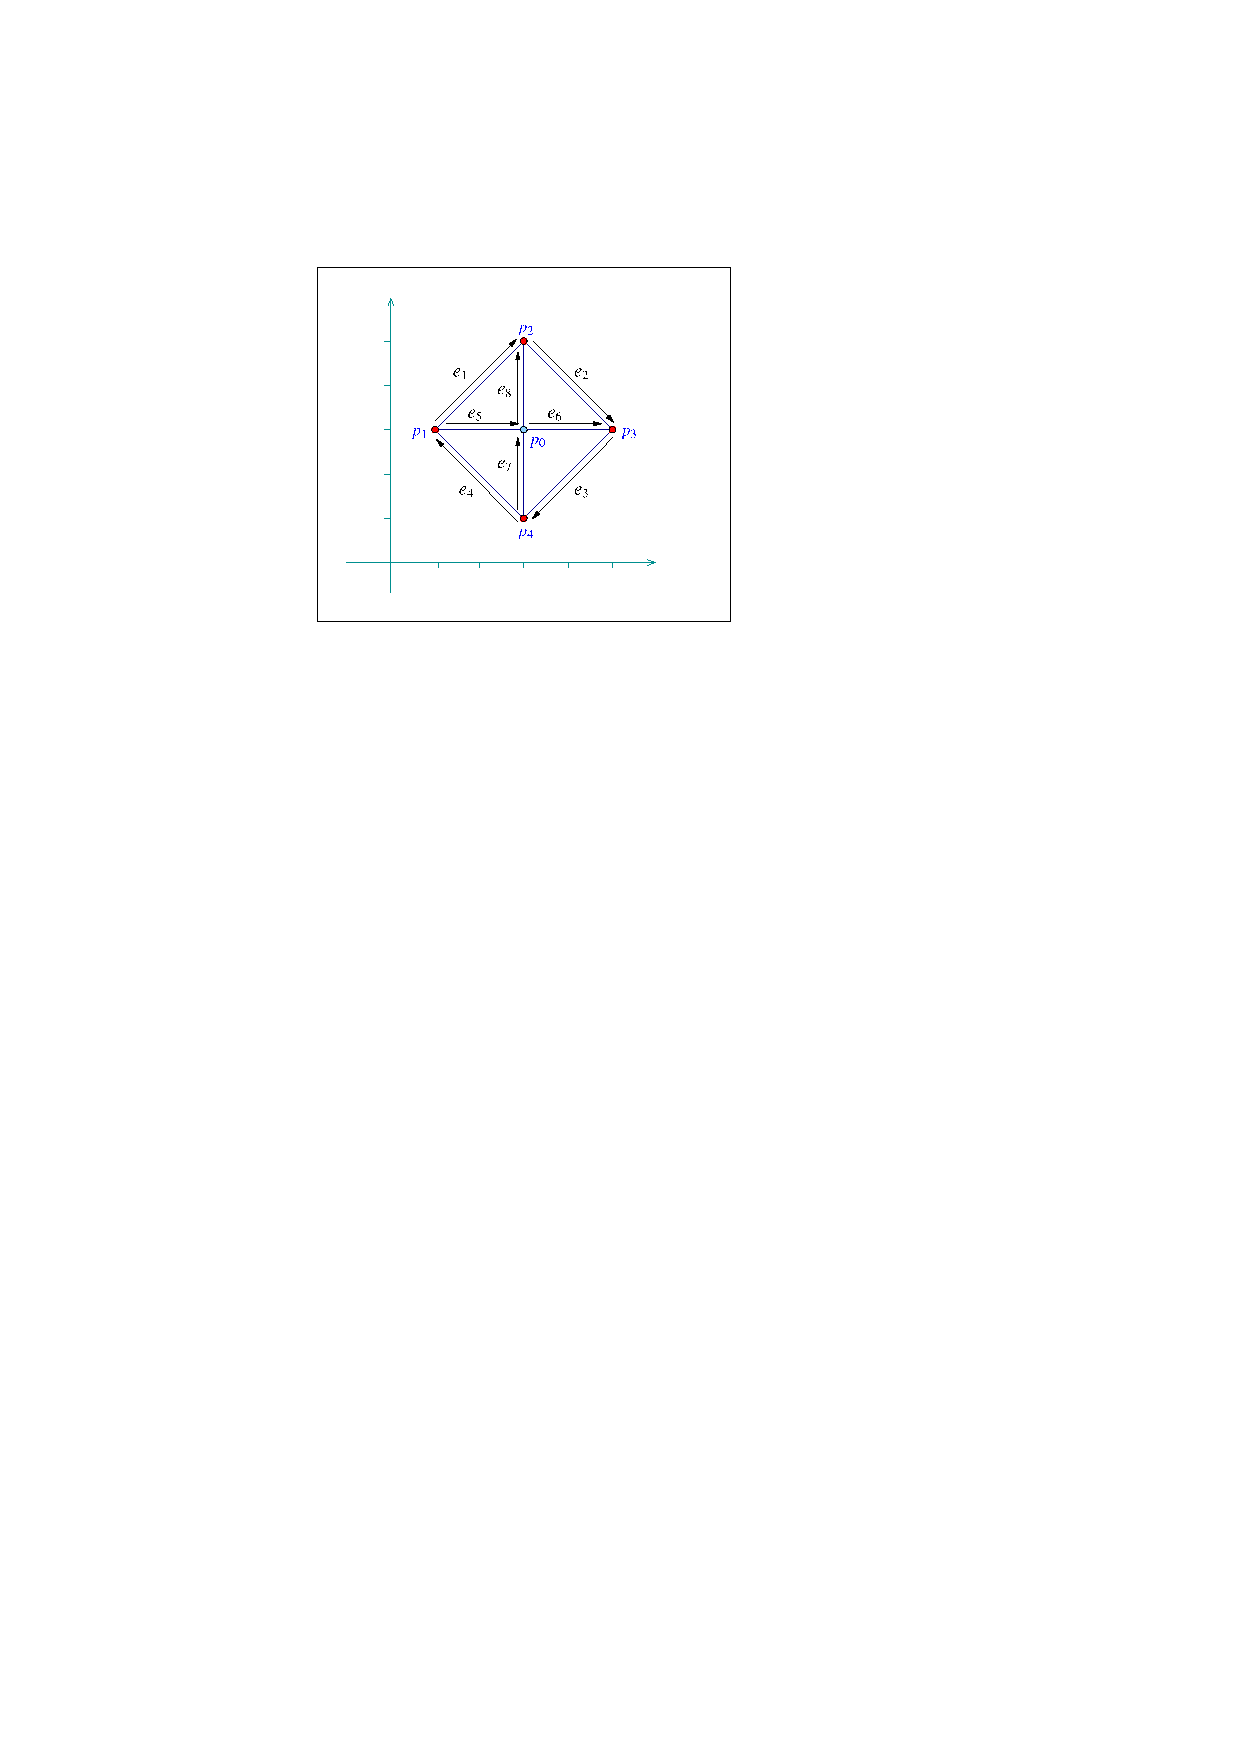
\includegraphics{Arrangement_2/fig/ex_4}
  \end{center}
\end{ccTexOnly}
\begin{ccHtmlOnly}
  <p><center>
  <img src="./fig/ex_4.gif" border=0 alt="Example 4">
  </center>
\end{ccHtmlOnly}
\caption{An arrangement of line segments, as constructed in
\ccc{ex_special_edge_insertion.C}. Note that $p_0$ is initially inserted as an
isolated point and later on connected to the other four vertices.}
\label{arr_fig:ex_4}
\end{figure}

\begin{ccHtmlOnly}<p>\end{ccHtmlOnly}
The following program shows how to construct the arrangement
depicted in Figure~\ref{arr_fig:ex_4} using the specialized
insertion functions that accept predecessor halfedges:

\ccIncludeExampleCode{../examples/Arrangement_2/ex_special_edge_insertion.C}

\begin{ccHtmlOnly}<p>\end{ccHtmlOnly}
It is possible to perform even more refined operations on an
\ccc{Arrangement_2} instance given specific topological information.
As most of these operations are very fragile and perform no precondition
testing on their input in order to gain efficiency, they are not included
in the public interface of the arrangement class. Instead, the
\ccc{Arr_accessor<Arrangement>} class allows access to these internal
arrangement operations --- see more details in the Reference Manual.
\end{ccAdvanced}

\section{Issuing Queries on an Arrangement}
\label{arr_sec:queries}
%==========================================
%
One of the most important query types defined on arrangements is
the {\em point-location} query: Given a point, find the
arrangement cell that contains it. Typically, the result of a
point-location query is one of the arrangement faces, but in
degenerate situations the query point can be located on an edge or
coincide with a vertex.

\begin{ccHtmlOnly}<p>\end{ccHtmlOnly}
Point-location queries are not only common in many applications,
they also play an important role in the free insertion-functions
(see Section~\ref{arr_sec:gl_funcs}). Therefore, it is crucial to
have the ability to answer such queries effectively for any
arrangement instance.

\subsection{Point-Location Queries}
\label{arr_ssec:pl}
%----------------------------------
%
The arrangement package includes several classes (more precisely,
class templates parameterized by an arrangement class) that model
the \ccc{ArrangementPointLocation_2} concept. Namely, they all
have a member function called \ccc{locate(q)} that accepts a query
point $q$ and result with a \cgal\ \ccc{Object} that wraps a handle
to the arrangement cell containing the query point. This object can
be assigned to either a \ccc{Face_const_handle},
\ccc{Halfedge_const_handle} or a \ccc{Vertex_const_handle}, depending
on whether the query point is located inside a face, on an edge or
on a vertex.

\begin{ccHtmlOnly}<p>\end{ccHtmlOnly}
Note that the handles returned by the \ccc{locate()} functions are
\ccc{const} (non-mutable) handles. If necessary, such handles may
be casted to mutable handles using the static functions
\ccc{Arrangement_2::non_const_handle()} provided by the
arrangement class.

\begin{ccHtmlOnly}<p>\end{ccHtmlOnly}
An instance of any point-location class must be attached to an
\ccc{Arrangement_2} instance so we can use it to issue point-location
queries. This attachment can be performed when the point-location
instance is constructed, or at a later time, using the \ccc{init(arr)}
method, where \ccc{arr} is the attached \ccc{Arrangement_2} instance.
In this chapter we always use the first option.

\begin{ccHtmlOnly}<p>\end{ccHtmlOnly}
The following function template, which can be found in the example
file \ccc{point_location_utils.h}, accepts a point-location object
(whose type can be any of the models to the
\ccc{ArrangementPointLocation_2} concept) and a query point, and
prints out the result of the point-location query for the given
point. Observe how we use the function \ccc{CGAL::assign()} is order
to cast the resulting \ccc{CGAL::Object} into a handle to an arrangement
feature. The point-location object \ccc{pl} is assumed to be already
associated with an arrangement:

\begin{alltt}
template <class PointLocation>
void point_location_query
        (const PointLocation& pl,
         const typename PointLocation::Arrangement_2::Point_2& q)
\{
  // Perform the point-location query.
  CGAL::Object obj = pl.locate (q);

  // Print the result.
  typedef typename PointLocation::Arrangement_2  Arrangement_2;

  typename Arrangement_2::Vertex_const_handle    v;
  typename Arrangement_2::Halfedge_const_handle  e;
  typename Arrangement_2::Face_const_handle      f;

  std::cout << "The point " << q << " is located ";
  if (CGAL::assign (f, obj)) \{
    // q is located inside a face:
    if (f->is_unbounded())
      std::cout << "inside the unbounded face." << std::endl;
    else
      std::cout << "inside a bounded face." << std::endl;
  \}
  else if (CGAL::assign (e, obj)) \{
    // q is located on an edge:
    std::cout << "on an edge: " << e->curve() << std::endl;
  \}
  else if (CGAL::assign (v, obj)) \{
    // q is located on a vertex:
    if (v->is_isolated())
      std::cout << "on an isolated vertex: " << v->point() << std::endl;
    else
      std::cout << "on a vertex: " << v->point() << std::endl;
  \}
  else \{
    CGAL_assertion_msg (false, "Invalid object.");
  \}
\}
\end{alltt}

\subsubsection{Choosing a Point-Location Strategy}
\label{arr_sssec:pl_strat}
%~~~~~~~~~~~~~~~~~~~~~~~~~~~~~~~~~~~~~~~~~~~~~~~~~
%
Each of the various point-location classes employs a different
algorithm or {\em strategy}\footnote{We use the term {\em strategy}
following the design pattern taxonomy~\cite{cgal:ghjv-dpero-95}.}
for answering queries:
\begin{itemize}
\item \ccc{Arr_naive_point_location<Arrangement>} locates the query
point \naive ly, by exhaustively scanning all arrangement cells.
%
\item \ccc{Arr_walk_along_a_line_point_location<Arrangement>}
simulates a traversal, in reverse order, along an imaginary vertical
ray emanating
from the query point: It starts from the unbounded face of the
arrangement and moves downward toward the query point until
locating the arrangement cell containing it.
%
\item \ccc{Arr_landmarks_point_location<Arrangement,Generator>}
uses a set of ``landmark'' points whose location in the
arrangement is known. Given a query point, it uses a \kdtree\ to
find the nearest landmark and then traverses the straight line
segment connecting this landmark to the query point.

\begin{ccHtmlOnly}<p>\end{ccHtmlOnly}
There are various ways to select the landmark set in the
arrangement, determined by the \ccc{Generator} template parameter.
By default, the generator
class \ccc{Arr_landmarks_vertices_generator} is used and the
arrangement vertices are the selected landmarks, but other
landmark generators, such as sampling random points or
choosing points on a grid, are also available; see the
reference manual for more details.
%
\item \ccc{Arr_trapezoid_ric_point_location<Arrangement>} implements
Mulmuley's point-location algorithm~\cite{m-fppa-90} (see
also~\cite[Chapter~6]{bkos-cgaa-00}). The
arrangement faces are decomposed into simpler cells of constant
complexity known as {\em pseudo-trapezoids} and a search-structure
(a directed acyclic graph) is constructed on top of these cells,
allowing to locate the pseudo-trapezoid (hence the arrangement
cell) containing a query point in expected logarithmic time.
\end{itemize}

\begin{ccHtmlOnly}<p>\end{ccHtmlOnly}
The main advantage of the first two strategies is that they do not
require any extra data, so the respective classes just store a
pointer to an arrangement object and operate directly on it.
Attaching such point-location objects to an existing arrangement
has virtually no running-time cost at all, but the query time is
linear in the size of the arrangement (the performance of the
``walk'' strategy is much better in practice, but its worst-case
performance is linear). Using these strategies is therefore
recommended only when a relatively small number of point-location
queries are issued by the application, or when the arrangement is
constantly changing (i.e., changes in the arrangement structure
are more frequent than point-location queries).

\begin{ccHtmlOnly}<p>\end{ccHtmlOnly}
On the other hand, the landmarks and the trapezoid RIC strategies
require auxiliary data structures on top of the arrangement, which
they need to construct once they are attached to an arrangement
object and need to keep up-to-date as this arrangement changes.
The data structures needed by both strategies can be constructed
in $O(N \log N)$ time (where $N$ is the overall number of edges in
the arrangement),
but the construction needed by the landmark algorithm is in
practice significantly faster. In addition, although both
resulting data structures are asymptotically linear in size, the
\kdtree\ that the landmark algorithm stores needs significantly
less memory. We note that Mulmuley's algorithm guarantees a
logarithmic query time, while the query time for the landmark
strategy is only logarithmic on average --- and we may have
scenarios where the query time can be linear. In practice however,
the query times of both strategies are competitive. For a detailed
experimental comparison, see \cite{idit-alenex}

\begin{ccHtmlOnly}<p>\end{ccHtmlOnly}
The main drawback in the current implementation of the landmark
strategy, compared to the trapezoidal RIC strategy, is that while
the updating the auxiliary data structures
related to the trapezoidal decomposition is done very efficiently,
the \kdtree\ maintained by the landmark algorithm needs to be
frequently rebuilt as the arrangement changes. In addition, using
the landmark point-location class adds some extra requirement
from the traits class (that is, the traits class should be a model
of a refined concept \ccc{ArrangementLandmarkTraits_2}; see
Section~\ref{arr_sec:traits} for the details). However, most
built-in traits classes that come with the \cgal\ public release
support these extra operations.

\begin{ccHtmlOnly}<p>\end{ccHtmlOnly}
It is therefore recommended to use the
\ccc{Arr_landmarks_point_location} class when the application
frequently issues point-location queries on an
arrangement that only seldom changes. If the arrangement is more
dynamic and is frequently going through changes, the
\ccc{Arr_trapezoid_ric_point_location} class should be the
selected point-location strategy.

\subsubsection{An Example}
\label{arr_sssec:pl_ex}
%~~~~~~~~~~~~~~~~~~~~~~~~~
%
\begin{figure}[!htp]
\begin{ccTexOnly}
  \begin{center}
  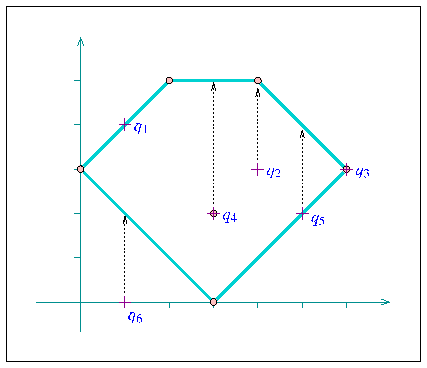
\includegraphics{Arrangement_2/fig/ex_5}
  \end{center}
\end{ccTexOnly}
\begin{ccHtmlOnly}
  <p><center>
  <img src="./fig/ex_5.gif" border=0 alt="Example 5">
  </center>
\end{ccHtmlOnly}
\caption{The arrangement of line segments, as constructed in
\ccc{ex_point_location.C}, \ccc{ex_vertical_ray_shooting.C}, and
\ccc{ex_batched_point_location.C}. The
arrangement vertices are drawn as small discs, while the query
points $q_1, \ldots, q_6$ are marked with crosses.}
\label{arr_fig:ex_5}
\end{figure}

\begin{ccHtmlOnly}<p>\end{ccHtmlOnly}
The following program constructs a simple arrangement of five line
segments that form a pentagonal face, with a single isolated
vertex in its interior, as depicted in Figure~\ref{arr_fig:ex_5}
(the arrangement construction is performed by the function
\ccc{construct_segment_arr()} whose listing is omitted here and
can be found in \ccc{point_location_utils.h}).
It then employs the \naive\ and the landmark strategies to issue
several point-location queries on this arrangement:

\ccIncludeExampleCode{../examples/Arrangement_2/ex_point_location.C}

\begin{ccHtmlOnly}<p>\end{ccHtmlOnly}
Note that the program uses the auxiliary
\ccc{point_location_query()} function template to nicely print the
result of each query. This function can be found in the header file
\ccc{point_location_utils.h}.

\subsection{Vertical Ray Shooting}
\label{arr_ssec:ray_shoot}
%---------------------------------
%
Another important query issued on arrangements is the vertical
ray-shooting query: Given a query point, which arrangement feature
do we encounter if we shoot a vertical ray emanating upward (or
downward) from this point? In the general case the ray hits an
edge, but it is possible that it hits a vertex, or that the
arrangement does not have any feature lying directly above (or
below) the query point.

\begin{ccHtmlOnly}<p>\end{ccHtmlOnly}
All point-location classes listed in the previous section are also models
of the \ccc{ArrangementVerticalRayShoot_2} concept. That is, they all
have member functions called \ccc{ray_shoot_up(q)} and
\ccc{ray_shoot_down(q)} that accept a query point $q$ and output a
\cgal\ \ccc{Object}. This can be assigned to either a
\ccc{Halfedge_const_handle} or to a \ccc{Vertex_const_handle}.
Alternatively, the returned value is a \ccc{Face_const_handle}
for the unbounded face of the arrangement, in case there is no edge
or vertex lying directly above (or below) $q$.

\begin{ccHtmlOnly}<p>\end{ccHtmlOnly}
The following function template, \ccc{vertical_ray_shooting_query()},
which also located in the header file \ccc{point_location_utils.h},
accepts a vertical ray-shooting
object, whose type can be any of the models to the
\ccc{ArrangementVerticalRayShoot_2} concept and prints out the
result of the upward vertical ray-shooting operations from a given
query point. The ray-shooting object \ccc{vrs} is assumed to be
already associated with an arrangement:

\begin{alltt}
template <class VerticalRayShoot>
void vertical_ray_shooting_query
    (const VerticalRayShoot& vrs,
     const typename VerticalRayShoot::Arrangement_2::Point_2& q)
\{
  // Perform the point-location query.
  CGAL::Object    obj = vrs.ray_shoot_up (q);

  // Print the result.
  typedef typename VerticalRayShoot::Arrangement_2  Arrangement_2;

  typename Arrangement_2::Vertex_const_handle    v;
  typename Arrangement_2::Halfedge_const_handle  e;
  typename Arrangement_2::Face_const_handle      f;

  std::cout << "Shooting up from " << q << " : "; 
  if (CGAL::assign (e, obj)) \{
    // We hit an edge:
    std::cout << "hit an edge: " << e->curve() << std::endl;
  \}
  else if (CGAL::assign (v, obj)) \{
    // We hit a vertex:
    if (v->is_isolated())
      std::cout << "hit an isolated vertex: " << v->point() << std::endl;
    else
      std::cout << "hit a vertex: " << v->point() << std::endl;
  \}
  else if (CGAL::assign (f, obj)) \{
    // We did not hit anything:
    CGAL_assertion (f->is_unbounded());
    
    std::cout << "hit nothing." << std::endl; 
  \}
  else \{
    CGAL_assertion_msg (false, "Invalid object.");
  \}
\}
\end{alltt}

\begin{ccHtmlOnly}<p>\end{ccHtmlOnly}
The following program uses the auxiliary function listed above to
perform vertical ray-shooting queries on an arrangement.
The arrangement and the query points are exactly the same as in
\ccc{ex_point_location.C} (see Figure~\ref{arr_fig:ex_5}):

\ccIncludeExampleCode{../examples/Arrangement_2/ex_vertical_ray_shooting.C}

\begin{ccHtmlOnly}<p>\end{ccHtmlOnly}
The number type we use in this example is \cgal's built-in
\ccc{MP_Float} type which is a floating-point number with an
unbounded mantissa and a 32-bit exponent. It supports construction from an
integer or from a machine \ccc{float} or \ccc{double} and performs additions,
subtractions and multiplications in an exact number.

\subsection{Batched Point-Location}
\label{arr_ssec:batched_pl}
%----------------------------------
%
Suppose that at a given moment our application has to issue a
relatively large number $m$ of point-location queries on a
specific arrangement instance. It is possible of course to define
a point-location object and to issue separate queries on the
arrangement. However, as explained in Section~\ref{arr_ssec:pl},
choosing a simple point-location strategy (either the \naive\ or
the walk strategy) means inefficient queries, while the more
sophisticated strategies need to construct auxiliary structures
that incur considerable overhead in running time.

\begin{ccHtmlOnly}<p>\end{ccHtmlOnly}
On the other hand, the arrangement package includes a free
\ccc{locate()} function that accepts an arrangement a range of
query points as its input and sweeps through the arrangement to
locate all query points in one pass. The function outputs the query
results as pairs, where each pair is comprised of a query point
and a \cgal\ \ccc{Object} that represents the cell containing the
point (see Section~\ref{arr_ssec:pl}). The output pairs are
sorted in increasing $xy$-lexicographical order of the query point.

\begin{ccHtmlOnly}<p>\end{ccHtmlOnly}
The batched point-location operation can be performed in
$O\left((m+N)\log{(m+N)}\right)$ time, where $N$ is the number of
edges in the arrangement. This means that when the number $m$ of
point-location queries is of the same order of magnitude as $N$,
this operation is more efficient than issuing separate queries.
This suggestion is also backed up by experimental results.
Moreover, the batched point-location operation is also
advantageous as it does not have to construct and maintain
additional data structures.

\begin{ccHtmlOnly}<p>\end{ccHtmlOnly}
The following program issues a batched point-location query, which
is essentially equivalent to the six separate queries performed in
\ccc{ex_point_location.C} (see Section~\ref{arr_ssec:pl}):

\ccIncludeExampleCode{../examples/Arrangement_2/ex_batched_point_location.C}

\section{Free Functions in the Arrangement Package}
\label{arr_sec:gl_funcs}
%==================================================
%
In Section~\ref{arr_sec:arr_class} we reviewed in details the
\ccc{Arrangement_2} class, which represents two-dimensional
subdivisions induced by bounded planar curves, and mentioned that its
interface is minimal in the sense that the member functions hardly
perform any geometric algorithms and are mainly used for
maintaining the topological structure of the subdivision. In this
section we explain how to utilize the free (global) functions that operate
on arrangements. The implementation of these operations typically require
non-trivial geometric algorithms or load some extra requirements on
the traits class.

\subsection{Incremental Insertion Functions}
\label{arr_ssec:inc_insert}
%-------------------------------------------
%
\subsubsection{Inserting Non-Intersecting Curves}
\label{arr_sssec:insert_non_x}
%~~~~~~~~~~~~~~~~~~~~~~~~~~~~~~~~~~~~~~~~~~~~~~~~
%
In Section~\ref{arr_sec:arr_class} we explained how to construct
arrangements of $x$-monotone curves that are pairwise disjoint in
their interior, when the location of the segment endpoints in the
arrangement is known. Here we relax this constraint, and allow the
location of the inserted $x$-monotone curve endpoints to be arbitrary,
as it may be unknown at the time of insertion. We retain, for the moment,
the requirement that the interior of the inserted curve is disjoint from
all existing arrangement edges and vertices.

\begin{ccHtmlOnly}<p>\end{ccHtmlOnly}
The free function \ccc{insert_non_intersecting_curve(arr, c, pl)}
inserts the $x$-monotone curve $c$ into the arrangement \ccc{arr},
with the precondition that the interior of $c$ is disjoint from
all \ccc{arr}'s existing edges and vertices. The third argument
\ccc{pl} is a point-location object attached to the arrangement,
which is used for performing the insertion. It locates both curve
endpoints in the arrangement, where each endpoint is expected to
either coincide with an existing vertex or lie inside a face.
It is possible to invoke one of the specialized insertion functions
(see Section~\ref{arr_sec:arr_class}), based on the query results, and
insert $c$ at its proper position.\footnote{The
\ccc{insert_non_intersecting_curve()} function, as all other functions
reviewed in this section, is a function template, parameterized by an
arrangement class and a point-location class (a model of the
\ccc{ArrangementPointLocation_2} concept).} The insertion operation
thus hardly requires any geometric operations on top on the ones
needed to answer the point-location queries. Moreover, it is
sufficient that the arrangement class is instantiated with a
traits class that models the \ccc{ArrangementBasicTraits_2}
concept (or the \ccc{ArrangementLandmarkTraits_2} concept, if the
landmark point-location strategy is used), which does not have to
support the computation of intersection points between curves.

\begin{ccHtmlOnly}<p>\end{ccHtmlOnly}
The variant \ccc{insert_non_intersecting_curve(arr, c)} is also
available. Instead of accepting a user-defined point-location
object, it defines a local instance of the walk point-location
class and uses it to insert the curve.

\subsubsection{Inserting $x$-Monotone Curves}
\label{arr_sssec:insert_x_mon}
%~~~~~~~~~~~~~~~~~~~~~~~~~~~~~~~~~~~~~~~~~~~~
%
The \ccc{insert_non_intersecting_curve()} function is very
efficient, but its preconditions on the input curves are still
rather restricting. Let us assume that the arrangement is
instantiated with a traits class that models the refined
\ccc{ArrangementXMonotoneTraits_2} concept and supports
intersection computations (see Section~\ref{arr_sec:traits} for
the exact details). Given an $x$-monotone curve, it is sufficient
to locate its left endpoint in the arrangement and to trace its
{\em zone}, namely the set of arrangement features crossing the curve,
until the right endpoint is reached. Each time the new curve $c$
crosses an existing vertex or an edge, the curve is split into
subcurves (in the latter case, we have to split the curve 
associated with the existing halfedge as well) and associate new
edges with the resulting subcurves. Recall that an edge is represented
by a pair of twin halfedges, so we split it into two halfedge pairs.

\begin{ccHtmlOnly}<p>\end{ccHtmlOnly}
The free function \ccc{insert_x_monotone_curve(arr, c, pl)} performs
this insertion operation. It accepts an $x$-monotone curve $c$,
which may intersect some of the curves already in the arrangement
\ccc{arr}, and inserts it into the arrangement by computing its zone.
Users may supply a point-location object \ccc{pl}, or use the default
walk point-location strategy (namely, the variant
\ccc{insert_x_monotone_curve(arr, c)} is also available). The
running-time of this insertion function is proportional to the
complexity of the zone of the curve $c$.

\begin{ccAdvanced}
In some cases users may have a prior knowledge of the location of the
left endpoint of the $x$-monotone curve \ccc{c} they wish to insert,
so they can perform the insertion without issuing any point-location
queries. This can be done by calling
\ccc{insert_x_monotone_curve(arr, c, obj)}, where \ccc{obj} is an
object represents the location of \ccc{c}'s left endpoint in the
arrangement --- namely it wraps a \ccc{Vertex_const_handle}, a
\ccc{Halfedge_const_handle} or a \ccc{Face_const_handle} (see
also Section~\ref{arr_ssec:pl}).
\end{ccAdvanced}

\subsubsection{Inserting General Curves}
\label{arr_sssec:insert_gen}
%~~~~~~~~~~~~~~~~~~~~~~~~~~~~~~~~~~~~~~~
%
So far all our examples were of arrangements of line segments,
where the \ccc{Arrangement_2} template was instantiated with the
\ccc{Arr_segment_traits_2} class. In this case, the fact that
\ccc{insert_x_monotone_curve()} accepts an $x$-monotone curve does not
seem to be a restriction, as all line segments are $x$-monotone
(note that we consider vertical line segments to be {\em weakly}
$x$-monotone).

\begin{ccHtmlOnly}<p>\end{ccHtmlOnly}
Suppose that we construct an arrangement of circles. A circle is
obviously not $x$-monotone, so we cannot use
\ccc{insert_x_monotone_curve()} in this case.\footnote{Note that a key
operation performed by \ccc{insert_x_monotone_curve()} is to locate the
left endpoint of the curve in the arrangement. A circle, however, does
not have any endpoints!} However, it is possible to subdivide each circle
into two $x$-monotone circular arcs (its upper half and its lower
half) and to insert each $x$-monotone arc separately.

\begin{ccHtmlOnly}<p>\end{ccHtmlOnly}
The free function \ccc{insert_curve()} requires that the traits class
used by the arrangement \ccc{arr} to be a model of the concept
\ccc{ArrangementTraits_2}, which refines the
\ccc{ArrangementXMonotoneTraits_2} concept. It has to define an
additional \ccc{Curve_2} type (which may differ from the
\ccc{X_monotone_curve_2} type), and support the subdivision of curves
of this new type into $x$-monotone curves (see the exact details in
Section~\ref{arr_sec:traits}). The \ccc{insert_curve(arr, c, pl)}
function performs the insertion of the curve $c$, which does not need
to be $x$-monotone, into the arrangement by subdividing it into
$x$-monotone subcurves and inserting each one separately. Users
may supply a point-location object \ccc{pl}, or use the default
walk point-location strategy by calling \ccc{insert_curve(arr, c)}.

\subsubsection{Inserting Points}
\label{arr_sssec:insert_point}
%~~~~~~~~~~~~~~~~~~~~~~~~~~~~~~~
%
The arrangement class enables us to insert a point as an isolated
vertex in a given face. The free function
\ccc{insert_point(arr, p, pl)} inserts a vertex into \ccc{arr} that
corresponds to the point \ccc{p} at an arbitrary location. It uses
the point-location object \ccc{pl} to locate the point in the
arrangement (by default, the walk point-location strategy is used),
and acts according to the result as follows:
\begin{itemize}
\item If \ccc{p} is located inside a face, it is inserted as an
isolated vertex inside this face.
\item If \ccc{p} lies on an edge, the edge is split to create a
vertex associated with \ccc{p}.
\item Otherwise, \ccc{p} coincides with an existing vertex and
we are done.
\end{itemize}
In all cases, the function returns a handle to the vertex
associated with \ccc{p}.

\begin{ccHtmlOnly}<p>\end{ccHtmlOnly}
The arrangement \ccc{arr} should be instantiated with a traits class
that models the \ccc{ArrangementXMonotoneTraits_2} concept, as the
insertion operation may involve splitting curves.

\subsubsection{An Example}
\label{arr_sssec:insert_ex}
%~~~~~~~~~~~~~~~~~~~~~~~~~~
%
\begin{figure}[!htp]
\begin{ccTexOnly}
  \begin{center}
  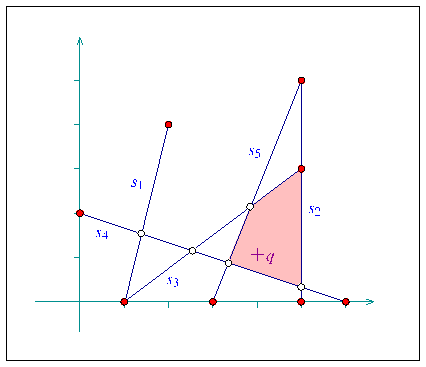
\includegraphics{Arrangement_2/fig/ex_8}
  \end{center}
\end{ccTexOnly}
\begin{ccHtmlOnly}
  <p><center>
  <img src="./fig/ex_8.gif" border=0 alt="Example 8">
  </center>
\end{ccHtmlOnly}
\caption{An arrangement of five intersecting line segments, as
constructed in \ccc{exincrementa_insertion.C} and
\ccc{ex_aggregated_insertion.C}. The segment
endpoints are marked by black disks and the arrangement vertices
that correspond to intersection points are marked by circles.
The query point $q$ is marked with a cross and the face that
contains it is shaded.}
\label{arr_fig:ex_8}
\end{figure}

\begin{ccHtmlOnly}<p>\end{ccHtmlOnly}
The program below constructs an arrangement of intersecting
line-segments. We know that $s_1$ and $s_2$ do not intersect, so
we use \ccc{insert_non_intersecting_curve()} to insert them into the
empty arrangement. The rest of the segments are inserted using
\ccc{insert_x_monotone_curve()} or \ccc{insert_curve()}, which are
equivalent in case of line segments. The resulting arrangement consists
of $13$ vertices, $16$ edges, and $5$ faces, as can be seen in
Figure~\ref{arr_fig:ex_8}.

\begin{ccHtmlOnly}<p>\end{ccHtmlOnly}
In the earlier examples, all arrangement vertices corresponded to
segment endpoints. In this example we have additional vertices that
correspond to intersection points between two segments. The
coordinates of these intersection points are rational numbers, if
the input coordinates are rational (or integer). Therefore,
the \ccc{Quotient<int>} number type is used to represent the
coordinates:

\ccIncludeExampleCode{../examples/Arrangement_2/ex_incremental_insertion.C}

\subsection{Aggregated Insertion Functions}
\label{arr_ssec:agg_insert}
%------------------------------------------
%
Let us assume that we have to insert a set of $m$ input curves into an
arrangement. It is possible to do this incrementally, 
inserting the curves one by one, as shown in the previous section.
However, the arrangement package provides three free functions that
aggregately insert a range of curves into an arrangement:
%
\begin{itemize}
\item \ccc{insert_non_intersecting_curves(arr, begin, end)} inserts 
a range of $x$-monotone curves given by the input iterators
\ccc{[begin, end)} into an arrangement \ccc{arr}. The $x$-monotone
curves should be pairwise disjoint in their interior and also
interior-disjoint from all existing edges and vertices of \ccc{arr}.
%
\item \ccc{insert_x_monotone_curves(arr, begin, end)} operates on
a range of $x$-monotone curves that may intersect one another.
%
\item \ccc{insert_curves(arr, begin, end)} inserts a range of
of general (not necessarily $x$-monotone) curves of type \ccc{Curve_2},
given by the input iterators \ccc{[begin, end)}, into the arrangement
\ccc{arr}.
\end{itemize}

\begin{ccHtmlOnly}<p>\end{ccHtmlOnly}
We distinguish between two cases: (i) The given arrangement
\ccc{arr} is empty (has only an unbounded face), so we have to
construct it from scratch. (ii) We have to insert $m$ input curves
to a non-empty arrangement \ccc{arr}.

\begin{ccHtmlOnly}<p>\end{ccHtmlOnly}
In the first case, we sweep over the input curves, compute
their intersection points and construct the \dcel\ that represents
their planar arrangement. This process is performed in
$O\left((m + k)\log m\right)$ time, where $k$ is the total number
of intersection points. The running time is asymptotically better
than the time needed for incremental insertion, if the arrangement
is relatively sparse (when $k$ is bounded by $\frac{m^2}{\log
m}$), but in practice it is recommended to use this aggregated
construction process even for dense arrangements, since the
sweep-line algorithm needs less geometric operations compared to
the incremental insertion algorithms and hence typically runs 
much faster in practice.

\begin{ccHtmlOnly}<p>\end{ccHtmlOnly}
Another important advantage the aggregated insertion functions
have is that they do not issue point-location queries. Thus, no
point-location object needs to be attached to the arrangement. As
explained in Section~\ref{arr_ssec:pl}, there is a trade-off
between construction time and query time in each of the
point-location strategies, which affects the running times of the
incremental insertion process. Naturally, this trade-off is irrelevant
in case of aggregated insertion as above.

\begin{ccHtmlOnly}<p>\end{ccHtmlOnly}
The example below shows how to construct the arrangement of
line segments depicted in Figure~\ref{arr_fig:ex_8} and built
incrementally in \ccc{ex_incremental_insertion.C}, as shown in the previous
section. We use the aggregated insertion function
\ccc{insert_x_monotone_curves()} as we deal with line segments.
Note that no point-location object needs to be defined and attached to the
arrangement:

\ccIncludeExampleCode{../examples/Arrangement_2/ex_aggregated_insertion.C}

\begin{ccHtmlOnly}<p>\end{ccHtmlOnly}
In case we have to insert a set of $m$ curves into an existing
arrangement, where we denote the number of edges in the arrangement by $N$.
As a rule of thumb, if $m = o(\sqrt{N})$, we insert the curves one by
one. For larger input sets, we use the aggregated insertion procedures.

\begin{figure}[!htp]
\begin{ccTexOnly}
  \begin{center}
  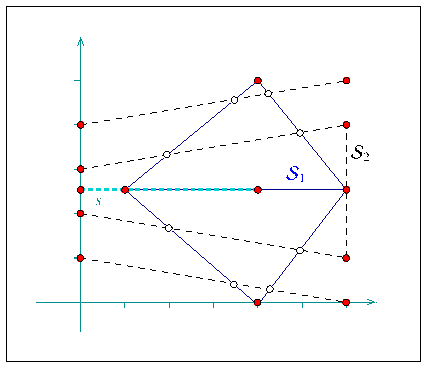
\includegraphics{Arrangement_2/fig/ex_10}
  \end{center}
\end{ccTexOnly}
\begin{ccHtmlOnly}
  <p><center>
  <img src="./fig/ex_10.gif" border=0 alt="Example 10">
  </center>
\end{ccHtmlOnly}
\caption{An arrangement of intersecting line segments, as
constructed in \ccc{ex_global_insertion.C}. The segments of ${\mathcal S}_1$
are drawn in solid lines and the segments of ${\mathcal S}_2$ are
drawn in dark dashed lines. Note that the segment $s$ (light
dashed line) overlaps one of the segments in ${\mathcal S}_1$.}
\label{arr_fig:ex_10}
\end{figure}

\begin{ccHtmlOnly}<p>\end{ccHtmlOnly}
In the example below we aggregately construct an arrangement of a set
${\mathcal S}_1$ containing five line segments. Then we insert a single
segment using the incremental insertion function. Finally, we add a set
${\mathcal S}_2$ with five more line segments in an aggregated fashion.
Notice that the line segments of ${\mathcal S}_1$ are pairwise
interior-disjoint, so we use \ccc{insert_non_intersecting_curves()}.
${\mathcal S}_2$ also contain pairwise interior-disjoint segments,
but as they intersect the existing arrangement, we have to use
\ccc{insert_x_monotone_curves()} to insert them. Also note that the
single segment $s$ we insert incrementally overlaps an existing
arrangement edge:

\ccIncludeExampleCode{../examples/Arrangement_2/ex_global_insertion.C}

\begin{ccHtmlOnly}<p>\end{ccHtmlOnly}
The number type used in the example above,
\ccc{Quotient<MP_Float>}, is capable of exactly computing the
intersection points as long as the segment endpoints are given as
floating-point numbers.

\subsection{Removing Vertices and Edges}
\label{arr_ssec:gl_remove}
%---------------------------------------
%
The free functions \ccc{remove_vertex()} and \ccc{remove_edge()} handle
the removal of vertices and edges from an arrangement. The difference
between these functions and the member functions of the \ccc{Arrangement_2}
template having the same name is that they allow the merger of two curves
associated with adjacent edges to form a single edge. Thus, they require
that the traits class that instantiates the arrangement instance is a model
of the refined \ccc{ArrangementXMonotoneTraits_2} concept (see
Section~\ref{arr_sec:traits}).

\begin{ccHtmlOnly}<p>\end{ccHtmlOnly}
The function \ccc{remove_vertex(arr, v)} removes the vertex
\ccc{v} from the given arrangement \ccc{arr}, where \ccc{v} is
either an isolated vertex or is a {\em redundant} vertex ---
namely, it has exactly two incident edges that are associated with
two curves that can be merged to form a single $x$-monotone curve.
If neither of the two cases apply, the function returns an
indication that it has failed to remove the vertex.

\begin{ccHtmlOnly}<p>\end{ccHtmlOnly}
The function \ccc{remove_edge(arr, e)} removes the edge \ccc{e}
from the arrangement by simply calling \ccc{arr.remove_edge(e)}
(see Section~\ref{arr_ssec:modify}). In addition, if either of the
end vertices of \ccc{e} becomes isolated or redundant after the removal
of the edge, it is removed as well.

\begin{ccHtmlOnly}<p>\end{ccHtmlOnly}
\begin{wrapfigure}[5]{r}{2.5cm}
\vspace{-2.8ex}
  \input{Arrangement_2/fig/h_shape.pstex_t}
\vspace{-1.8ex}
\end{wrapfigure}
%
The following example demonstrates the usage of the free removal
functions. In creates an arrangement of four line segment forming
an H-shape with a double horizontal line. Then it removes the two
horizontal edges and clears all redundant vertices, such that the
final arrangement consists of just two edges associated with the
vertical line segments:

\ccIncludeExampleCode{../examples/Arrangement_2/ex_global_removal.C}

\section{Traits Classes}
\label{arr_sec:traits}
%=======================
%
As mentioned in the introduction of this chapter, the traits class
encapsulates the definitions of the geometric entities and
implements the geometric predicates and constructions needed by
the \ccc{Arrangement_2} class and by its peripheral algorithms. We also
mention throughout the chapter that there are different levels of
requirements from the traits class, namely the traits class can model
different concept refinement-levels.

\begin{ccHtmlOnly}<p>\end{ccHtmlOnly}
A model of the basic concept, \ccc{ArrangementBasicTraits_2},
needs to define the types \ccc{Point_2} and
\ccc{X_monotone_curve_2}, where objects of the first type are
the geometric mapping of arrangement vertices, and objects of the
latter type are the geometric mapping of edges. In addition, it has to
support the following set of predicates:
\begin{itemize}
\item Compare the $x$-coordinates of two points $p$ and $q$.
\item Compare two points $p$ and $q$ lexicographically, by their
$x$-coordinates then by their $y$-coordinates.
\item Return the left endpoint (similarly, the right endpoint) of
an $x$-monotone curve $c$.
\item Given an $x$-monotone curve $c$ and a point $p$ that lies in its
$x$-range, determine whether $p$ lies below, above or on $c$.
\item Given two $x$-monotone curves $c_1$ and $c_2$ that share a
common left endpoint (similarly, right endpoint) $p$, determine
whether $c_1$ lies above or under $c_2$ immediately to the right
(to the left) of $p$, or whether the two curves coincide there.
\item Check two curves for equality (two curves are equal if their
graph is the same).
\end{itemize}
This basic set of predicates is sufficient for constructing
arrangements of $x$-monotone curves and points that are pairwise
disjoint in their interiors and for performing point-location
queries and vertical ray-shooting queries.

\begin{ccHtmlOnly}<p>\end{ccHtmlOnly}
The landmark point-location strategy (see
Section~\ref{arr_ssec:pl}) needs its associated arrangement to be
instantiated with a model of the refined
\ccc{ArrangementLandmarkTraits_2} traits concept. A model of this
concept must define a fixed precision number type (typically
\ccc{double}) and support the additional operations:
\begin{itemize}
\item Given a point \ccc{p}, approximate the $x$ and $y$-coordinates
of \ccc{p} using the fixed precision number type. We use this operation
for approximate computations --- there are certain operations in the
search for the location of the point that need not be exact and we can
perform them faster than other operations. 
\item Given two points $p_1$ and $p_2$, construct an $x$-monotone
curve connecting $p_1$ and $p_2$.
\end{itemize}

\begin{ccHtmlOnly}<p>\end{ccHtmlOnly}
A traits class that models the \ccc{ArrangementXMonotoneTraits_2}
concept, which refines the \ccc{ArrangementBasicTraits_2}
concept, has to support the following functions:
\begin{itemize}
\item Compute all intersection points and overlapping sections of
two given $x$-monotone curves. If possible, compute also the
multiplicity of each intersection point.\footnote{If the two
curves intersect at a point $p$ but have different tangents, $p$
is of multiplicity 1. If the tangents are also equal but the their
curvatures are not the same, $p$ is of multiplicity 2, etc.}
Knowing the multiplicity of an intersection point is not required,
but it can speed up the arrangement construction.
\item Split an $x$-monotone curve $c$ into two subcurves at a point
$p$ lying in the interior of $c$.
\item Given two $x$-monotone curve $c_1$ and $c_2$ that share a
common endpoint, determine whether $c_1$ and $c_2$ are {\em
mergeable}, that is, whether they can be merged to form a
single continuous $x$-monotone curve of the type supported by the
traits class.
\item Merge two mergeable $x$-monotone curve $c_1$ and $c_2$.
\end{itemize}
Using a model of the \ccc{ArrangementXMonotoneTraits_2}, it is
possible to construct arrangements of sets of $x$-monotone curves
(and points) in that may intersect one another.

\begin{ccHtmlOnly}<p>\end{ccHtmlOnly}
The concept \ccc{ArrangementTraits_2} refines the
\ccc{ArrangementXMonotoneTraits_2} concept by adding the notion
of a general, not necessarily $x$-monotone (and not necessarily
connected) curve. A model of this concept must define the
\ccc{Curve_2} type and support the division of a curve into a
set of continuous $x$-monotone curves and isolated points. For
example, the curve $C:\ (x^2 + y^2)(x^2 + y^2 - 1) = 0$ is the
unit circle (the loci of all points for which $x^2 + y^2  = 1$)
with the origin $(0,0)$ as a singular point in its interior. $C$
should therefore be divided into two circular arcs (the upper
part and the lower part of the unit circle) and a single isolated
point.

\begin{ccHtmlOnly}<p>\end{ccHtmlOnly}
Note that the refined model \ccc{ArrangementTraits_2} is required
only when using the free \ccc{insert_curve()} and
\ccc{insert_curves()} functions (see Section~\ref{arr_sec:gl_funcs}),
which accept a \ccc{Curve_2} object in the incremental version,
or a range of \ccc{Curve_2} objects in the aggregated version.
In all other cases it is sufficient to use a model of the
\ccc{ArrangementXMonotoneTraits_2} concept.

\begin{ccHtmlOnly}<p>\end{ccHtmlOnly}
In the rest of this section we review the traits classes
included in the public distribution of \cgal, that handle line
segments, polylines and conic arcs. The last subsection overviews
decorators for geometric traits classes distributed with \cgal,
which extend other geometric traits-class by attaching auxiliary
data with the geometric objects.

\subsection{Traits Classes for Line Segments}
\label{arr_ssec:tr_segs}
%-----------------------------------------
%
The \ccc{Arr_segment_traits_2<Kernel>} class used so far
in all example programs in this chapter is parameterized by a
geometric kernel and uses the \ccc{Kernel::Point_2} type as it
point type. However, nor the \ccc{Curve_2} neither the
\ccc{X_monotone_curve_2} types are identical to the
\ccc{Kernel::Segment_2} type. A kernel segment is typically
represented by its two endpoints, and these may have a large bit-size
representation, if the segment is intersected and split several
times (in comparison with the representation of its original
endpoints). The large representation may significantly slow down the
various traits-class operations involving such a segment. In contrast,
the \ccc{Arr_segment_traits_2} represents a segment using
its supporting line and the two endpoints, such that most computations
are performed on the supporting line, which never changes as the
segment is split. It also caches some additional information with
the segment to speed up various predicates.
An \ccc{X_monotone_curve_2} object can still be constructed from two
endpoints or from a kernel segment. Moreover, an
\ccc{X_monotone_curve_2} instance can also be casted or assigned to a
\ccc{Kernel::Segment_2} object. The two types are thus fully
convertible to one another.

\begin{ccHtmlOnly}<p>\end{ccHtmlOnly}
The arrangement package also offers a simpler alternative
segment-traits class. The traits class
\ccc{Arr_non_caching_segment_basic_traits<Kernel>} models 
the \ccc{ArrangementBasicTraits_2} concept. It uses
\ccc{Kernel::Point_2} as its point type and
\ccc{Kernel::Segment_2} as its $x$-monotone curve type. As this
traits class does not support intersecting and splitting segments,
the kernel representation is sufficient. It is still less
efficient than \ccc{Arr_segment_traits_2} for constructing
arrangements of pairwise disjoint line segments in many cases, as
it performs no caching at all, but using this traits class may be
preferable as it reduces the memory consumption a bit, since no extra
data is stored with the line segments.

\begin{ccHtmlOnly}<p>\end{ccHtmlOnly}
The class \ccc{Arr_non_caching_segment_traits<Kernel>} inherits
from \ccc{Arr_non_caching_segment_basic_traits<Kernel>} and
extends it to be a model of the \ccc{ArrangementTraits_2} concept.
It may thus be used to construct arrangement of intersecting line
segments, but as explained above, for efficiency reasons it is
recommended to use it only when the arrangement is very sparse and
contains hardly any intersection points.

\subsection{The Polyline Traits Class}
\label{arr_ssec:tr_polylines}
%-----------------------------------
%
The \ccc{Arr_polyline_traits_2<SegmentTraits>} class can be used
to maintain arrangements of polylines (a.k.a. poly-segments),
which are continuous piecewise linear curves. A polyline can be
created from a range of points, where the $i$-th and $(i+1)$-st
points in the range represent the endpoints of the $i$-th segment
of the polyline. The polyline traits class is parameterized with a
segment-traits class that supports the basic operations on
segments.

\begin{ccHtmlOnly}<p>\end{ccHtmlOnly}
Polylines are the simplest form of a curves that are not
necessarily $x$-monotone. They can be used to approximate more
complicated curves in a convenient manner, as the algebra needed
to handle them is elementary --- rational arithmetic is sufficient
to construct an arrangement of polylines is an exact and robust
manner. Note, however, that a single polyline can be split into
many $x$-monotone polylines, and that the number of intersection
points (or overlapping sections) between two polylines can also
be large. 

\begin{ccHtmlOnly}<p>\end{ccHtmlOnly}
The polyline-traits class is a model of the \ccc{ArrangementTraits_2}
concept and of the \ccc{ArrangementLandmarkTraits_2} concept.
It inherits its point type from the segment-traits class, and defines
the polyline type, which serves as its \ccc{Curve_2}. Polyline curve
objects can be constructed from a range of points. They also enable
the traversal over the range of defining points, whose first and
past-the-end iterators can be obtained through the methods \ccc{begin()}
and \ccc{end()}. The nested \ccc{X_monotone_curve_2} type inherits
from \ccc{Curve_2}. The points in an $x$-monotone curve are
always stored in lexicographically increasing order of their
coordinates.

\begin{figure}[!htp]
\begin{ccTexOnly}
  \begin{center}
  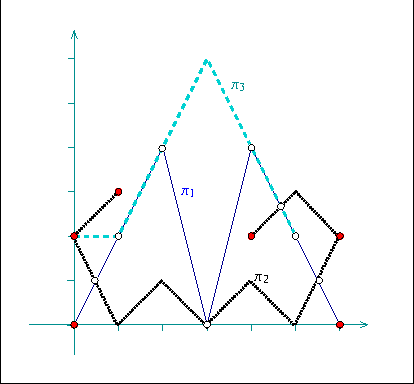
\includegraphics{Arrangement_2/fig/ex_12}
  \end{center}
\end{ccTexOnly}
\begin{ccHtmlOnly}
  <p><center>
  <img src="./fig/ex_12.gif" border=0 alt="Example 12">
  </center>
\end{ccHtmlOnly}
\caption{An arrangement of three polylines, as constructed in
\ccc{ex_polylines.C}. Disks mark vertices associated with
polyline endpoints, while circles mark vertices that correspond
to intersection points. Note that $\pi_2$ is split into three
$x$-monotone polylines, and that $\pi_1$ and $\pi_3$ have two
overlapping sections.}
\label{arr_fig:ex_12}
\end{figure}

\begin{ccHtmlOnly}<p>\end{ccHtmlOnly}
The following example program constructs an arrangement of three
polylines, as depicted in Figure~\ref{arr_fig:ex_12}. Note that
most points defining the polylines are not associated with arrangement
vertices. The arrangement vertices are either the extreme points of
each $x$-monotone polyline or the intersection points between two
polylines:

\ccIncludeExampleCode{../examples/Arrangement_2/ex_polylines.C}

\subsection{The Conic Traits Class}
\label{arr_ssec:tr_conic}
%-------------------------------
%
A {\em conic curve} is an algebraic curve of degree 2. Namely, it
is the locus of all points $(x,y)$ satisfying the equation $C:\ r
x^2 + s y^2 + t xy + u x + v y + w = 0$, where the six
coefficients $\langle r, s, t, u, v, w \rangle$ completely
characterize the curve. The sign of the expression $\Delta_{C} = 4
r s - t^2$ determines the type of curve:
\begin{itemize}
\item If $\Delta_{C} > 0$ the curve is an ellipse. A circle is a
special case of an ellipse, where $r = s$ and $t = 0$.
%
\item If $\Delta_{C} = 0$ the curve is a parabola --- an unbounded
conic curve with a single connected branch. When $r = s = t = 0$
we have a line, which can be considered as a degenerate parabola.
%
\item If $\Delta_{C} < 0$ the curve is a hyperbola. That is, it
is comprised of two disconnected unbounded branches.
\end{itemize}

\begin{ccHtmlOnly}<p>\end{ccHtmlOnly}
As the arrangement package is suitable for bounded curves, we
consider bounded segments of conic curves, referred to as {\em
conic arcs}. A conic arc $a$ may be either (i) a full ellipse, or
(ii) defined by the tuple $\langle C, p_s, p_t, o \rangle$, where
$C$ is a conic curve and $p_s$ and $p_t$ are two points on $C$
(namely $C(p_s) = C(p_t) = 0$) that define the {\em source} and
{\em target} of the arc, respectively. The arc is formed by
traversing $C$ from the source to the target going in the
orientation specified by $o$, which is typically clockwise or
counterclockwise orientation (but may also be collinear in case of
degenerate conic curves).

\begin{ccHtmlOnly}<p>\end{ccHtmlOnly}
We always assume that the conic coefficients $\langle r, s,
t, u, v, w \rangle$ are rational. When dealing with linear curves
(line segments and polylines), similar assumptions guarantee that
all intersection points also have rational coordinates, such that
the arrangement of such curves can be constructed and maintained
using only rational arithmetic. Unfortunately, this does not hold
for conic curves, as the coordinates of intersection points of two
conic curves with rational coefficients are in general algebraic
numbers of degree $4$.\footnote{Namely, they are roots of
polynomials with integer coefficients of degree $4$. However, in
some special cases, for example when handling only circles and
circular arcs, the coordinates of the intersection points are only
of degree $2$, namely they are solutions of quadratic equations.}
In addition, conic arcs may not necessarily be $x$-monotone, and
must be split at points where the tangent to the arc is vertical.
In the general case, such points typically have coordinates that
are algebraic numbers of degree $2$.
It is therefore clear that we have to use different number types
to represent the conic coefficients and the point coordinates.
Note that as arrangement vertices induced by intersection points
and points with vertical tangents are likely to have algebraic
coordinates, we also allow the original endpoints of the input arcs
$p_s$ and $p_t$ to have algebraic coordinates.

\begin{ccHtmlOnly}<p>\end{ccHtmlOnly}
The \ccc{Arr_conic_traits_2<RatKernel, AlgKernel, NtTraits>} class
template is designed for efficient handling of arrangements of
bounded conic arcs. The template has three parameters, defined as
follows:
\begin{itemize}
\item The \ccc{RatKernel} class is a geometric kernel, whose field
type is an exact rational type. It is used to define basic
geometric entities (e.g., a line segment or a circle) with rational
coefficients. Typically we use one of the standard \cgal\ kernels,
instantiated with the number type \ccc{NtTraits::Rational} (see
below).
%
\item The \ccc{AlgKernel} class is a geometric kernel whose field
type is an exact algebraic type. It is used to define points with
algebraic coordinates. Typically we use one of the standard
\cgal\ kernels, instantiated with the number type
\ccc{NtTraits::Algebraic} (see below).
%
\item The \ccc{NtTraits} class (the number-type traits class)
encapsulates all the numeric operations needed for performing the
geometric computation carried out by the geometric traits class.
It defines the \ccc{Integer}, \ccc{Rational} and \ccc{Algebraic}
number-types, and supports several operations on these types, such
as conversion between number types, solving quadratic equations
and extracting the real roots of a polynomial with integer
coefficients. It is highly recommended to use the
\ccc{CORE_algebraic_number_traits} class, which is included in the
arrangement package. It relies on the exact number types
implemented in the {\sc Core} library and performs exact
computations on the number types it defines.
\end{itemize}

\begin{ccHtmlOnly}<p>\end{ccHtmlOnly}
The \ccc{Arr_conic_traits_2} models the \ccc{ArrangementTraits_2} and
the \ccc{ArrangementLandmarkTraits_2} concepts. (It supports
the landmark point-location strategy). Its \ccc{Point_2} type is
derived from \ccc{AlgKernel::Point_2}, while the \ccc{Curve_2}
type represents a bounded, not necessarily $x$-monotone, conic arc.
The \ccc{X_monotone_curve_2} type is derived from \ccc{Curve_2},
but its constructors are to be used only by the traits class.
Users should therefore construct only \ccc{Curve_2} objects and
insert them into the arrangement using the \ccc{insert_curve()}
or \ccc{insert_curves()} functions.

\begin{ccHtmlOnly}<p>\end{ccHtmlOnly}
Conic arcs can be constructed from full ellipses or by specifying
a supporting curve, two endpoints and an orientation. However,
several constructors of \ccc{Curve_2} are available to allow for some
special cases, such as circular arcs or line segments. The
\ccc{Curve_2} (and the derived \ccc{X_monotone_curve_2}) classes
also support basic access functions such as \ccc{source()},
\ccc{target()} and \ccc{orientation()}.

\subsubsection{Examples for Arrangements of Conics}
%~~~~~~~~~~~~~~~~~~~~~~~~~~~~~~~~~~~~~~~~~~~~~~~~~~
%
\begin{figure}[!htp]
\begin{ccTexOnly}
  \begin{center}
  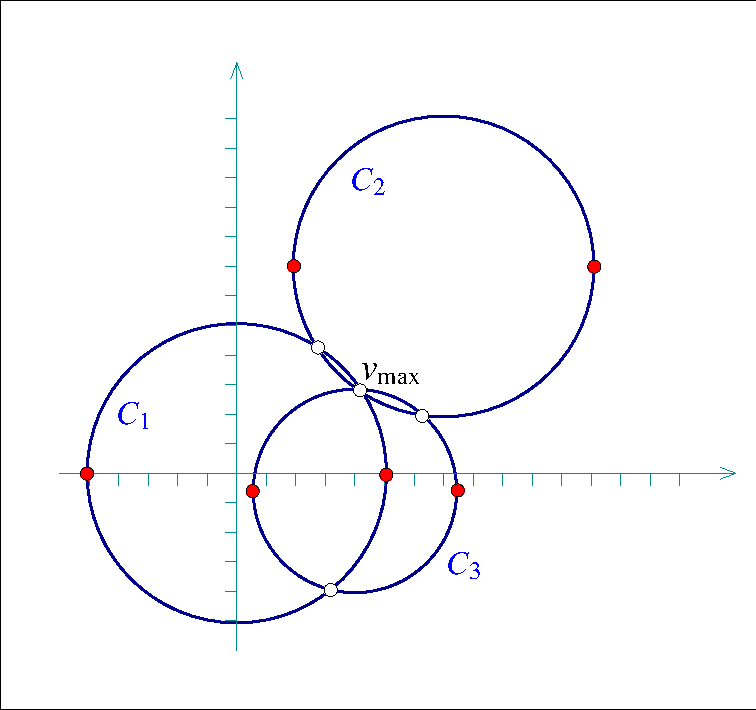
\includegraphics{Arrangement_2/fig/ex_13}
  \end{center}
\end{ccTexOnly}
\begin{ccHtmlOnly}
  <p><center>
  <img src="./fig/ex_13.gif" border=0 alt="Example 13">
  </center>
\end{ccHtmlOnly}
\caption{An arrangement of three circles constructed in
\ccc{ex_circles.C}. Each circle is split into two $x$-monotone
circular arcs, whose endpoints are drawn as disks. Circles
mark vertices that correspond to intersection points. The vertex
$v_{\rm max}$ is a common intersection point of all three
circles.}
\label{arr_fig:ex_13}
\end{figure}

\begin{ccHtmlOnly}<p>\end{ccHtmlOnly}
In the following example an arrangement of three full circles is
constructed, as shown in Figure~\ref{arr_fig:ex_13}. Then, the vertex
of maximal degree is searched for. The geometric mapping of this
vertex is the point $(4,3)$, as all three circles intersect at this point
and the associated vertex has six incident edges:

\ccIncludeExampleCode{../examples/Arrangement_2/ex_circles.C}

\begin{figure}[!htp]
\begin{ccTexOnly}
  \begin{center}
  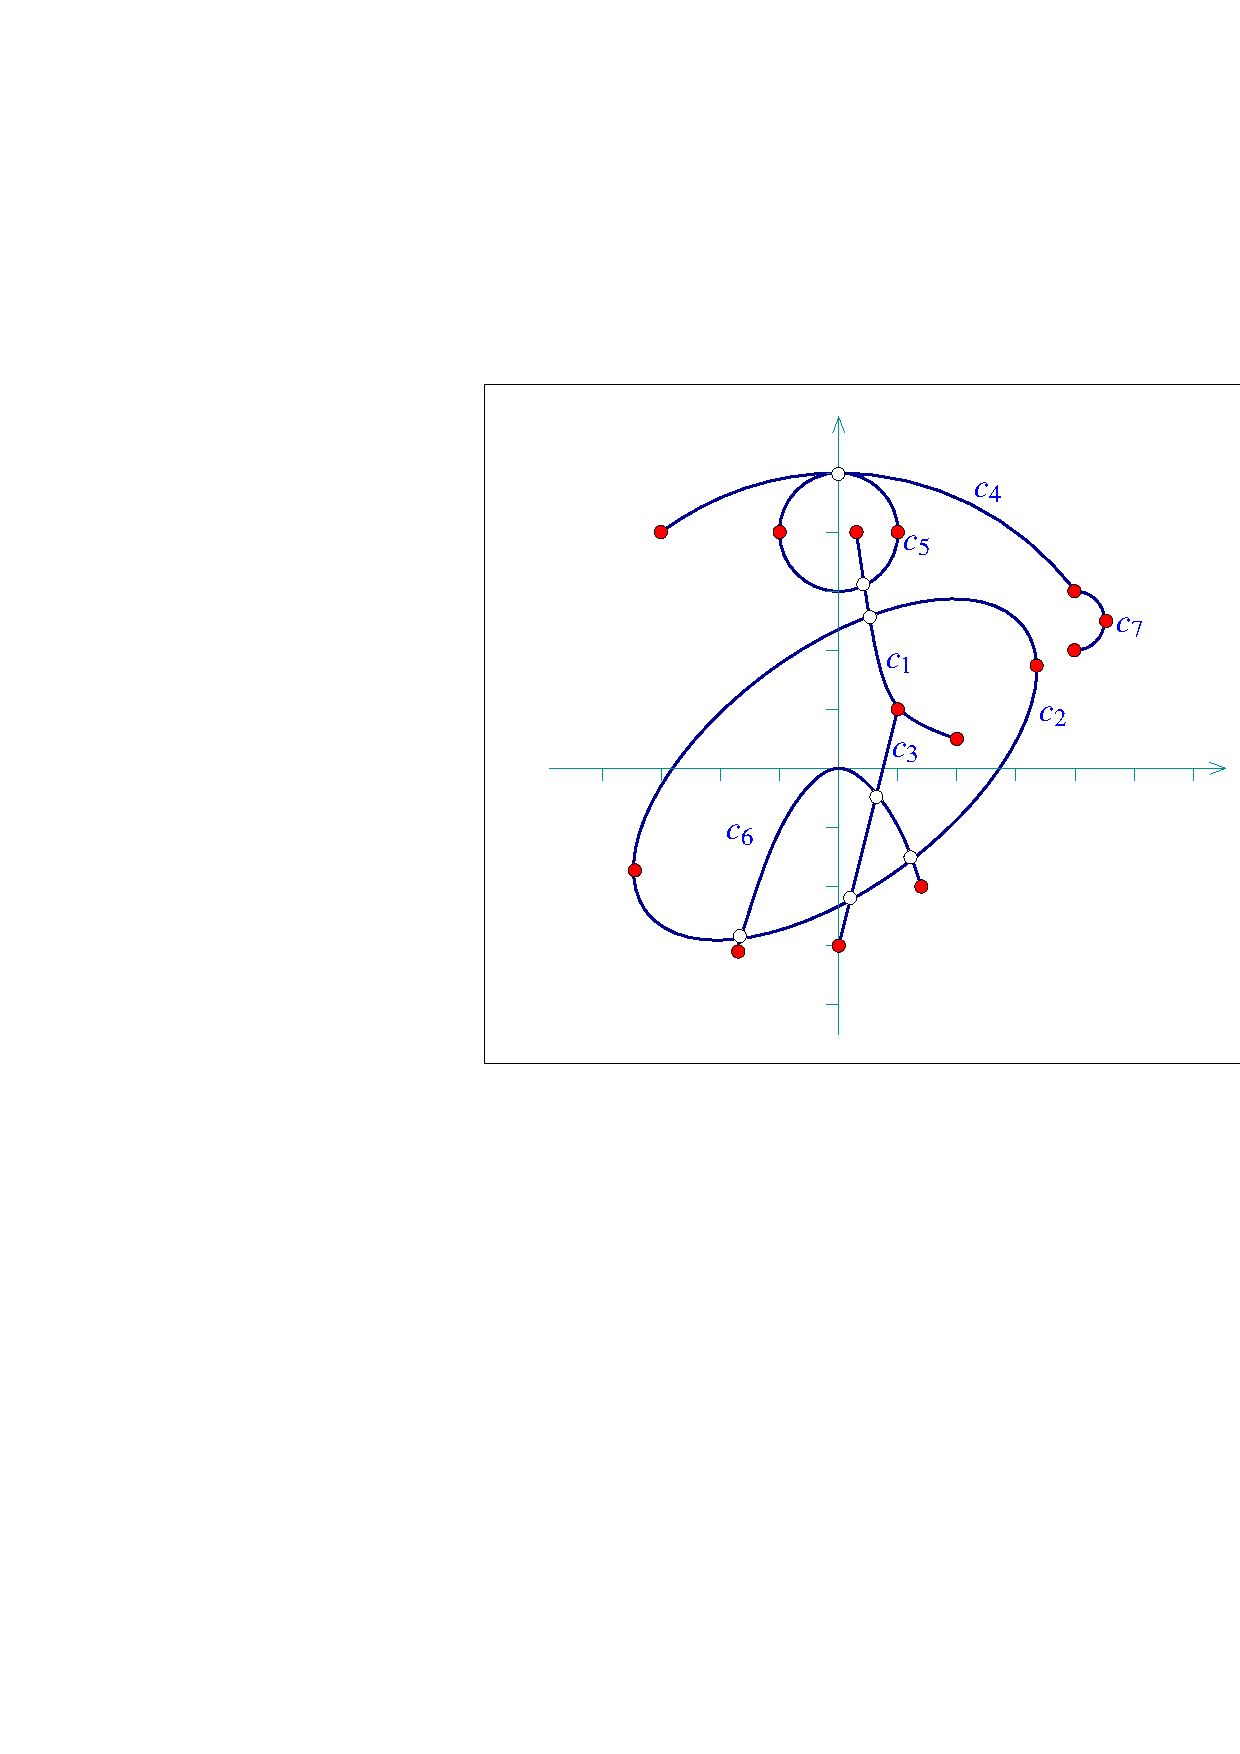
\includegraphics{Arrangement_2/fig/ex_14}
  \end{center}
\end{ccTexOnly}
\begin{ccHtmlOnly}
  <p><center>
  <img src="./fig/ex_14.gif" border=0 alt="Example 14">
  </center>
\end{ccHtmlOnly}
\caption{An arrangement of mixed conic arcs, as constructed in
\ccc{ex_conics.C}.}
\label{arr_fig:ex_14}
\end{figure}

\begin{ccHtmlOnly}<p>\end{ccHtmlOnly}
The following example demonstrates the usage of the various
constructors for conic arcs. The resulting arrangement is depicted
in Figure~\ref{arr_fig:ex_14}. Especially noteworthy are the
constructor of a circular arc that accepts three points and the
constructor that allows specifying approximate endpoints, where the
exact endpoints are given explicitly as intersections of
the supporting conic with two other conic curves. Also note that as the
preconditions required by some of these constructors are rather
complicated (see the reference manual for the details), a
precondition violation does not cause the program to terminate ---
instead, an {\em invalid} arc is created. We can verify the validity
of an arc by using the \ccc{is_valid()} method. Needless to say, inserting
invalid arcs into an arrangement is not allowed.

\ccIncludeExampleCode{../examples/Arrangement_2/ex_conics.C}

\begin{ccHtmlOnly}<p>\end{ccHtmlOnly}
The last example in this section demonstrates how the conic-traits
class can handle intersection points with multiplicity. The
supporting curves of the two arcs, a circle centered at
$(0,\frac{1}{2})$ with radius $\frac{1}{2}$, and the hyperbola $y
= \frac{x^2}{1-x}$,\footnote{This curve can also be written as $C:
x^2 + xy - y = 0$. It is a hyperbola since $\Delta_{C} = -1$.}
intersect at the origin such that the intersection point has
multiplicity $3$ (note that they both have the same horizontal
tangent at $(0,0)$ and the same curvature $1$). In addition, they
have another intersection point at $(\frac{1}{2},\frac{1}{2})$ of
multiplicity $1$:

\ccIncludeExampleCode{../examples/Arrangement_2/ex_conic_multiplicities.C}

\subsection{Traits Class for Arcs of Rational Functions}
\label{arr_ssec:tr_ratfunc}
%-------------------------------------------------------
%
A {\em rational function} is given by the equation $y =
\frac{P(x)}{Q(x)}$, where $P$ and $Q$ are polynomials of arbitrary
degrees. In particular, if $Q(x) = 1$, then the function is a
simple polynomial function. A bounded {\em rational arc} is
defined by the graph of a rational function over some interval
$[x_{\rm min}, x_{\rm max}]$, where $Q$ does not have any real
roots in this interval (Thus, the arc does not contain any poles).
Rational functions, and polynomial functions in particular, are
not only interesting in their own right, they are also very useful
for approximating or interpolating more complicated curves; see,
e.g.,~\cite[Chapter~3]{cgal:ptvf-nrcpp-02}.

\begin{ccHtmlOnly}<p>\end{ccHtmlOnly}
The computations with rational arcs are guaranteed to be robust and 
exact, assuming that the coefficient of the polynomials $P$ and $Q$
are rational  numbers. The $x$-values that determine the interval
over which the arc is defined can however be arbitrary algebraic
numbers.

\begin{ccHtmlOnly}<p>\end{ccHtmlOnly}
Using the \ccc{Arr_rational_traits_2<AlgKernel, NtTraits>} class
template it is possible to construct and maintain arrangement of
rational arcs. The template parameters are very similar to the
ones used by the \ccc{Arr_conic_traits_2} class template; see
the previous section. However, no rational kernel is needed. Also
in this case it is recommended to use the
\ccc{CORE_algebraic_number_traits} class, with a kernel templated
by the \ccc{Algebraic} type defined by this class.

\begin{ccHtmlOnly}<p>\end{ccHtmlOnly}
The \ccc{Arr_rational_traits_2} is a model of the
\ccc{ArrangementTraits_2} concept (but not of the
\ccc{ArrangementLandmarkTraits_2} concept, so it is not possible
to use the landmark point-location strategy for arrangements of
rational arcs). Its \ccc{Point_2} type is derived from
\ccc{AlgKernel::Point_2}, while the \ccc{Curve_2} and
\ccc{X_monotone_curve_2} types refer to the same class (note that
a rational arc is always $x$-monotone). The traits class also
defines the \ccc{Rat_vector} type, representing a vector of
rational coefficients, (whose type is \ccc{NtTraits::Rational}). A
rational arc can be constructed from a single vector of
coefficients, specifying the polynomial $P$ alone (and $Q(x) =
1$), or from two vectors of coefficients, specifying both $P$ and
$Q$.

\begin{figure}[!htp]
\begin{ccTexOnly}
  \begin{center}
  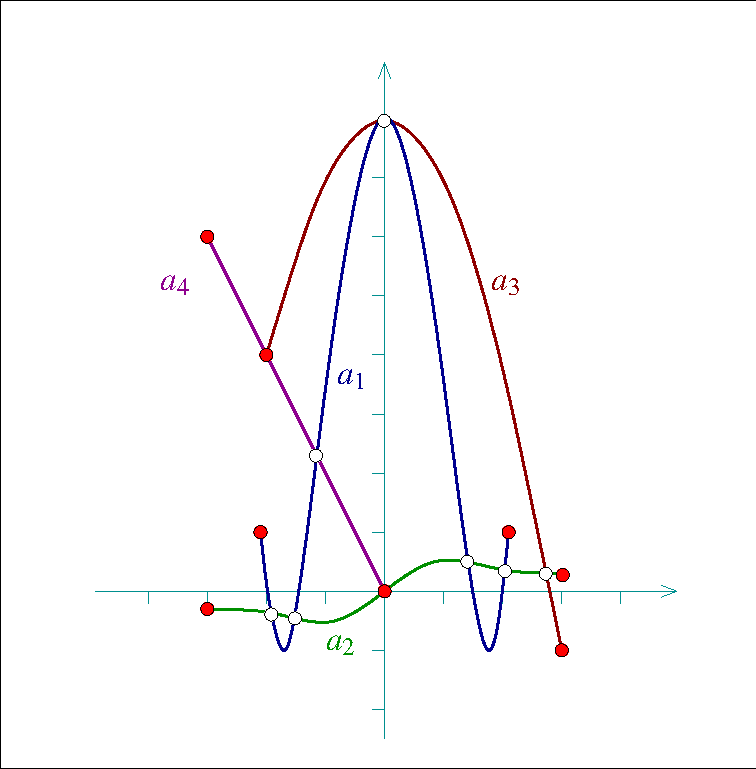
\includegraphics{Arrangement_2/fig/ex_16}
  \end{center}
\end{ccTexOnly}
\begin{ccHtmlOnly}
  <p><center>
  <img src="./fig/ex_16.gif" border=0 alt="Example 16">
  </center>
\end{ccHtmlOnly}
\caption{An arrangement of four arcs of rational functions, as
constructed in \ccc{ex_rational_functions.C}.}
\label{arr_fig:ex_16}
\end{figure}

\begin{ccHtmlOnly}<p>\end{ccHtmlOnly}
The following example demonstrates the construction of an
arrangement of rational arcs depicted in
Figure~\ref{arr_fig:ex_16}. Note the usage of the two
constructors, for polynomial arcs and for rational arcs:

\ccIncludeExampleCode{../examples/Arrangement_2/ex_rational_functions.C}

\subsection{Traits-Class Decorators}
\label{arr_ssec:meta_tr}
%-----------------------------------
%
Geometric traits-class decorators allow users to attach auxiliary
data to curves and to points. The data is automatically manipulated 
by the decorators and distributed to the constructed geometric entities. 
Note that additional information can alternatively be maintained by extending 
the vertex, halfedge, or face types provided by the \dcel\ class used 
by the arrangement; see the details in Section~\ref{arr_sec:ex_dcel}.

\begin{ccHtmlOnly}<p>\end{ccHtmlOnly}
The arrangement package includes a generic traits-class decorator
template named 
\ccc{Arr_curve_data_traits_2<BaseTraits, XMonotoneCurveData, Merge, CurveData, Convert>}.
This decorator is used to attach a data field to curves and to
$x$-monotone curves. It is parameterized by a base-traits class, which is
one of the geometric traits classes described in the previous subsections, or
a user-defined traits class. The curve-data decorator derives itself from the
base-traits class, and in particular inherits its \ccc{Point_2} type.
In addition:
\begin{itemize}
\item \ccc{Curve_2} is derived from the basic \ccc{BaseTraits::Curve_2}
class, extending it by an extra field of type \ccc{CurveData}.
%
\item \ccc{X_monotone_curve_2} is derived from the basic
\ccc{BaseTraits::X_monotone_curve_2} class, extending it by an extra field of
type \ccc{XMonotoneCurveData}.
\end{itemize}
Note that the \ccc{Curve_2} and \ccc{X_monotone_curve_2} are not
the same, even if the \ccc{BaseTraits::Curve_2} and
\ccc{BaseTraits::X_monotone_curve_2} are (as in the case of the 
segment-traits class for example). The extended curve types support the
additional methods \ccc{data()} and \ccc{set_data()} for
accessing and modifying the data field.

\begin{ccHtmlOnly}<p>\end{ccHtmlOnly}
Users can create an extended curve (or an extended $x$-monotone
curve) from a basic curve and a curve-data object. When curves are
inserted into an arrangement, they may be split, and the
decorator handles their data fields automatically:
\begin{itemize}
\item When a curve is subdivided into $x$-monotone subcurves, its
data field of type \ccc{CurveData} is converted to an \ccc{XMonotoneCurveData}
object $d$ using the \ccc{Convert} functor. The object $d$ is automatically
associated with each of the resulting $x$-monotone subcurves.

\begin{ccHtmlOnly}<p>\end{ccHtmlOnly}
Note that by default, the \ccc{CurveData} type is identical to the
\ccc{XMonotoneCurveData} type (and the conversion functor \ccc{Convert}
is trivially defined). Thus, the data field associated with the original
curve is just duplicated and stored with the $x$-monotone subcurves.
%
\item When an $x$-monotone curve is split into two, the decorator
class automatically copies its data field to both resulting subcurves.
%
\item When intersecting two $x$-monotone curves $c_1$ and $c_2$, the
result may include overlapping sections, represented as
$x$-monotone curves. In this case the data fields of $c_1$ and $c_2$
are merged into a single \ccc{XMonotoneCurveData} object,
using the \ccc{Merge} functor, which is supplied as a
parameter to the traits class-template. The resulting object is
assigned to the data field of the overlapping subcurves.
%
\item Merging two $x$-monotone curves is allowed only when (i)~the two
curves are geometrically mergeable --- that is, the base-traits class
allows to merge them --- and (ii)~the two curves store the same data field.
\end{itemize}

\begin{ccHtmlOnly}<p>\end{ccHtmlOnly}
The \ccc{Arr_consolidated_curve_data_traits_2<BaseTraits, Data>} decorator
specializes the generic curve-data decorator. It extends the basic
\ccc{BaseTraits::Curve_2} by a single \ccc{Data} field, and the basic
\ccc{BaseTraits::X_monotone_curve_2} with a {\em set} of (distinct) data 
objects. The \ccc{Data} type is required to support the equality operator, 
used to ensure that each set contains only distinct data objects with no 
duplicates.
When a curve with a data field $d$ is subdivided into $x$-monotone subcurves,
each subcurve is associated with a set $S = \{ d \}$. In case of an overlap
between two $x$-monotone curves $c_1$ and $c_2$ with associated data sets
$S_1$ and $S_2$, respectively, the overlapping subcurve is associated with
the consolidated set $S_1 \cup S_2$.

\subsubsection{Examples}
%~~~~~~~~~~~~~~~~~~~~~~~
%
\begin{figure}[!htp]
\begin{ccTexOnly}
  \begin{center}
  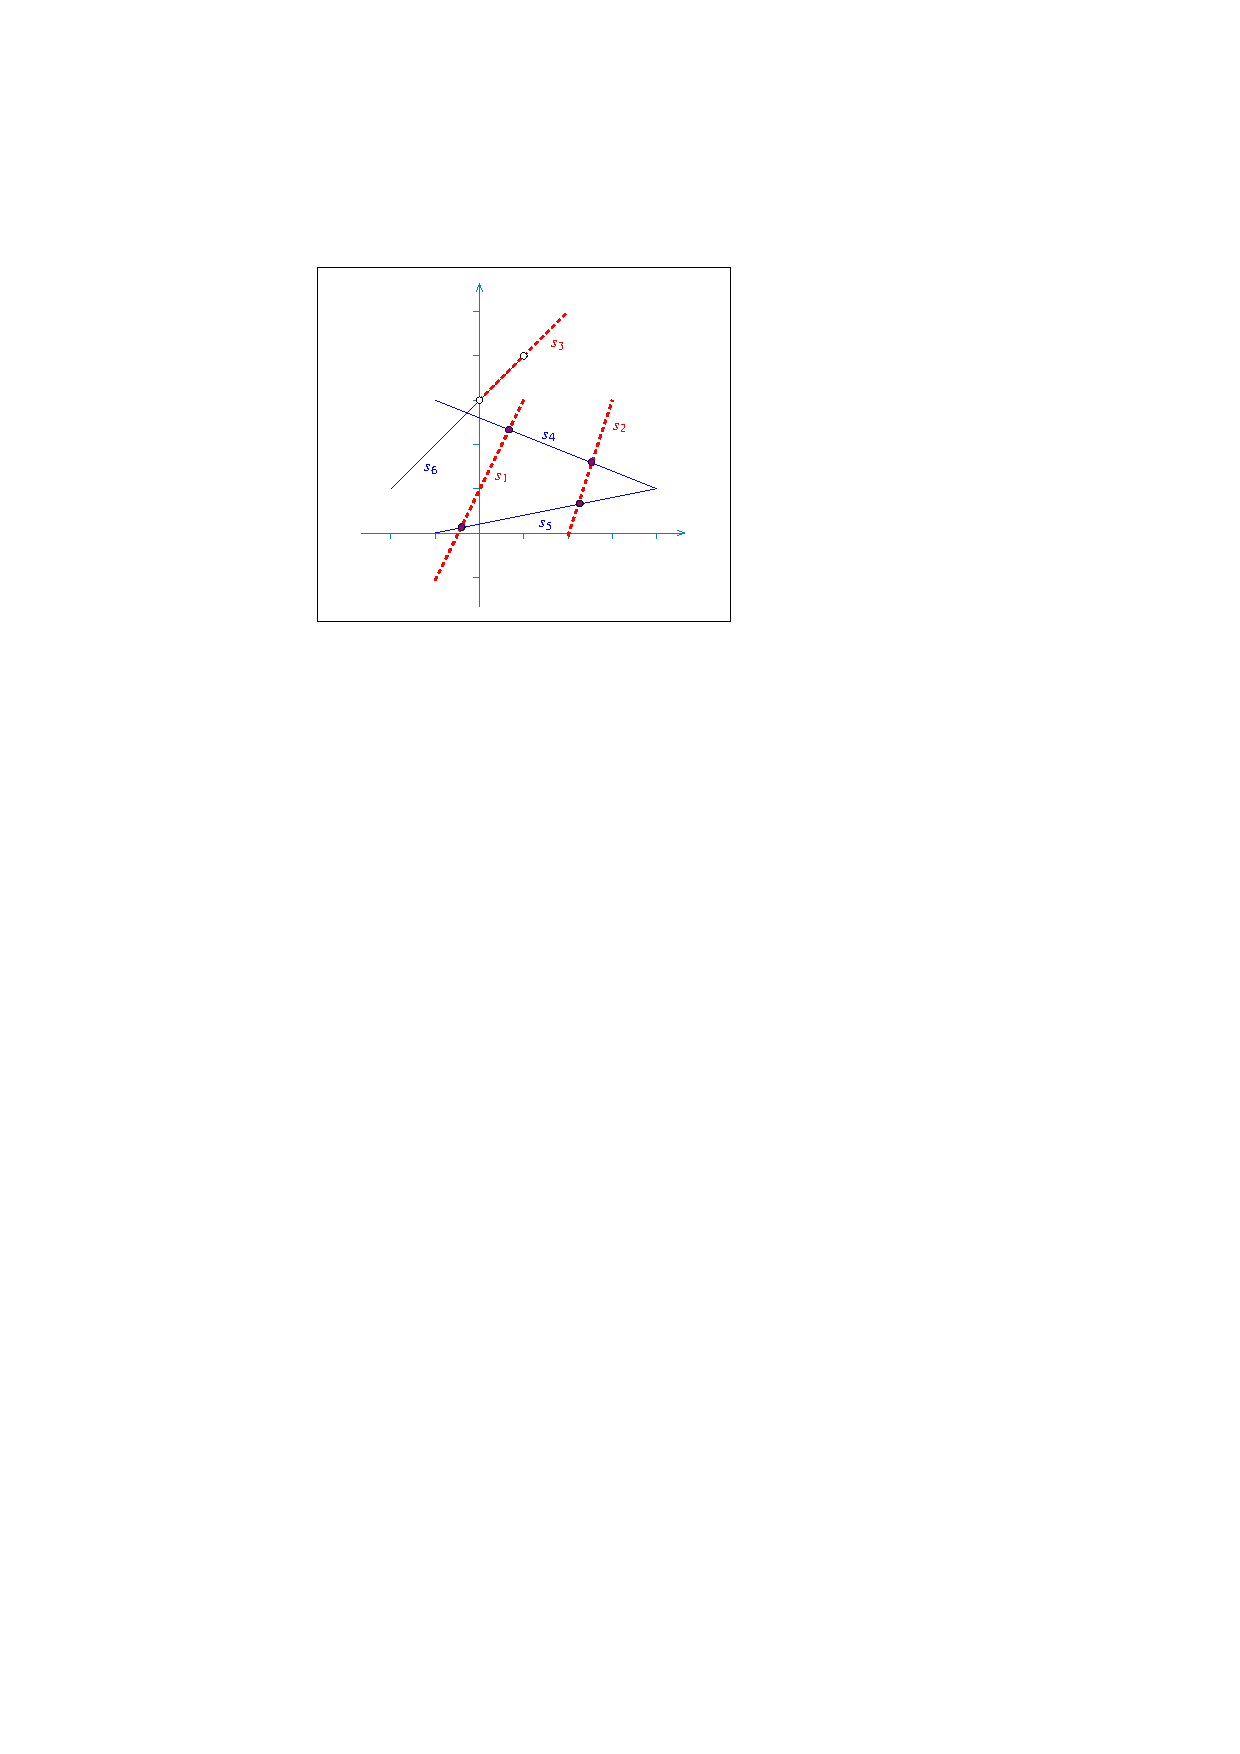
\includegraphics{Arrangement_2/fig/ex_17}
  \end{center}
\end{ccTexOnly}
\begin{ccHtmlOnly}
  <p><center>
  <img src="./fig/ex_17.gif" border=0 alt="Example 17">
  </center>
\end{ccHtmlOnly}
\caption{An arrangement of six red and blue segments, as
constructed in \ccc{ex_consolidated_curve_data.C}. Disks correspond to
red--blue intersection points, while circles mark the endpoints
of red--blue overlaps.}
\label{arr_fig:ex_17}
\end{figure}

\begin{ccHtmlOnly}<p>\end{ccHtmlOnly}
In the following example, we use \ccc{Arr_segment_traits_2} as our
base-traits class, attaching an additional {\em color} field to
the segments using the consolidated curve-data traits class. A
color may be either {\em blue} or {\em red}. Having constructed
the arrangement of colored segments, as depicted in
Figure~\ref{arr_fig:ex_17}, we detect the vertices that have incident 
edges mapped to both blue and red segments. Thus, they correspond
to red--blue intersection points. We also locate the edge that
corresponds to overlaps between red and blue line segments:

\ccIncludeExampleCode{../examples/Arrangement_2/ex_consolidated_curve_data.C}

\begin{figure}[!htp]
\begin{ccTexOnly}
  \begin{center}
  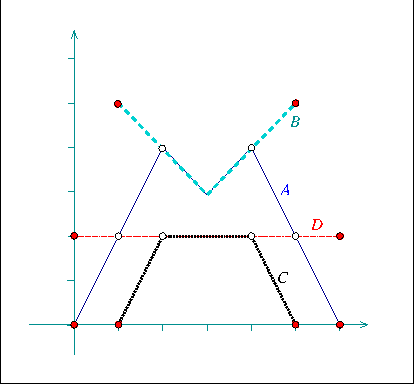
\includegraphics{Arrangement_2/fig/ex_18}
  \end{center}
\end{ccTexOnly}
\begin{ccHtmlOnly}
  <p><center>
  <img src="./fig/ex_18.gif" border=0 alt="Example 18">
  </center>
\end{ccHtmlOnly}
\caption{An arrangement of four polylines, named A--D, as
constructed in \ccc{ex_generic_curve_data.C}.}
\label{arr_fig:ex_18}
\end{figure}

\begin{ccHtmlOnly}<p>\end{ccHtmlOnly}
In the following example, we use \ccc{Arr_polyline_traits_2} as
our base-traits class, attaching an additional {\em name} field to
each polyline using the generic curve-data traits class. In case of
overlaps, we simply concatenate the names of the overlapping
polylines. Also notice how we replace the curve associated with
the edges that correspond to overlapping polylines with 
geometrically equivalent curves, but with a different data fields:

\ccIncludeExampleCode{../examples/Arrangement_2/ex_generic_curve_data.C}

\section{The Notification Mechanism}
\label{arr_sec:notif}
%===================================
%
For some applications it is essential to know exactly what
happens inside a specific arrangement-instance. For example, when
a new curve is inserted into an arrangement, it might be desired to keep
track of the faces that are split due to this insertion operation.
Other important examples are the point-location strategies that
require auxiliary data-structures (see Section~\ref{arr_ssec:pl}),
which must be notified on various local changes in the arrangement,
in order to keep their data structures up-to-date. The arrangement
package offers a mechanism that uses {\em observers} 
(see~\cite{cgal:ghjv-dpero-95}) that can be
attached to an arrangement instance and receive notifications
about the changes this arrangement goes through.

\begin{ccHtmlOnly}<p>\end{ccHtmlOnly}
The \ccc{Arr_observer<Arrangement>} class-template is
parameterized with an arrangement class. It stores a pointer to an
arrangement object, and is capable of receiving notifications {\em
just before} a structural change occurs in the arrangement and
{\em immediately after} such a change takes place.
\ccc{Arr_observer} serves as a base class for other observer
classes and defines a set of virtual notification functions,
giving them all a default empty implementation.

\begin{ccHtmlOnly}<p>\end{ccHtmlOnly}
The set of functions can be divided into three categories, as
follows:
\begin{enumerate}
\item Notifiers of changes that affect the entire topological structure
of the arrangement. This category consists of two pairs that
notify the observer of the following changes:
\begin{itemize}
\item The arrangement is cleared.
\item The arrangement is assigned with the contents of another
arrangement.
\end{itemize}
\item Pairs of notifiers of a local change that occurs in the
topological structure. Most notifier functions belong to this
category. The relevant local changes include:
\begin{itemize}
\item A new vertex is constructed and associated with a point.
\item An edge\footnote{The term ``edge'' refers here to a pair of twin
half-edges.} is constructed and associated with an $x$-monotone
curve.
\item An edge is split into two edges.
\item An existing face is split into two faces, as a consequence of the
insertion of a new edge.
\item A hole is created in the interior of a face.
\item Two holes are merged to form a single hole, as a consequence of the
insertion of a new edge.
\item A hole is moved from one face to another, as a consequence of
a face split.
\item Two edges are merged into one edge.
\item Two faces are merged into one face, as a consequence of the
removal of an edge that used to separate them.
\item One hole is split into two, as a consequence of the deletion of an 
edge that used to connect the two components.
\item A vertex is removed.
\item An edge is removed.
\item A hole is deleted from the interior of a face.
\end{itemize}
\item Notifiers about a change applied by a free (global) function.
This category consists of a single pair of notifiers, namely
\ccc{before_global_change()} and \ccc{after_global_change()}. Neither of
these functions is invoked by methods of the \ccc{Arrangement_2} class. 
Instead, they are called by the free functions themselves. It is implied 
that no point-location queries (or any other queries for that matter)
are issued between the calls to the notification functions above.
\end{enumerate}
See the reference manual for a detailed specification of the
\ccc{Arr_observer} class, along with the exact prototypes of all
notification functions.

\begin{ccHtmlOnly}<p>\end{ccHtmlOnly}
Each arrangement object stores a (possibly empty) list of pointers to
\ccc{Arr_observer} objects, and whenever one of the structural
changes listed in the first two categories above is about to take
place, the arrangement object performs a {\em forward} traversal
on this list and invokes the appropriate function of each
observer. After the change takes place the observer list is
traversed in a {\em backward} manner (from tail to head) and the
appropriate notification function is invoked for each observer.
This allows the nesting of observer objects.

\begin{ccHtmlOnly}<p>\end{ccHtmlOnly}
Concrete arrangement-observer classes should inherit from
\ccc{Arr_observer}. When an observer is constructed, it is attached to
a valid arrangement supplied to the observed constructor, or alternatively 
the observer can be attached to the arrangement at a later time.
When this happens, the observer instance adds itself to the
observer list of the associated arrangement and starts receiving
notifications whenever this arrangement changes tehreafter. Naturally,
the observer object unregisters itself by removing itself from
this list just before it is destroyed.

\begin{ccHtmlOnly}<p>\end{ccHtmlOnly}
The trapezoidal RIC and the landmark point-location strategies
both use observers to keep their auxiliary data structures
up-to-date. Besides them, users can define their own observer
classes, by inheriting from the base observer class and overriding
the relevant notification functions, as required by their
applications.

\begin{figure}[!htp]
\begin{ccTexOnly}
  \begin{center}
  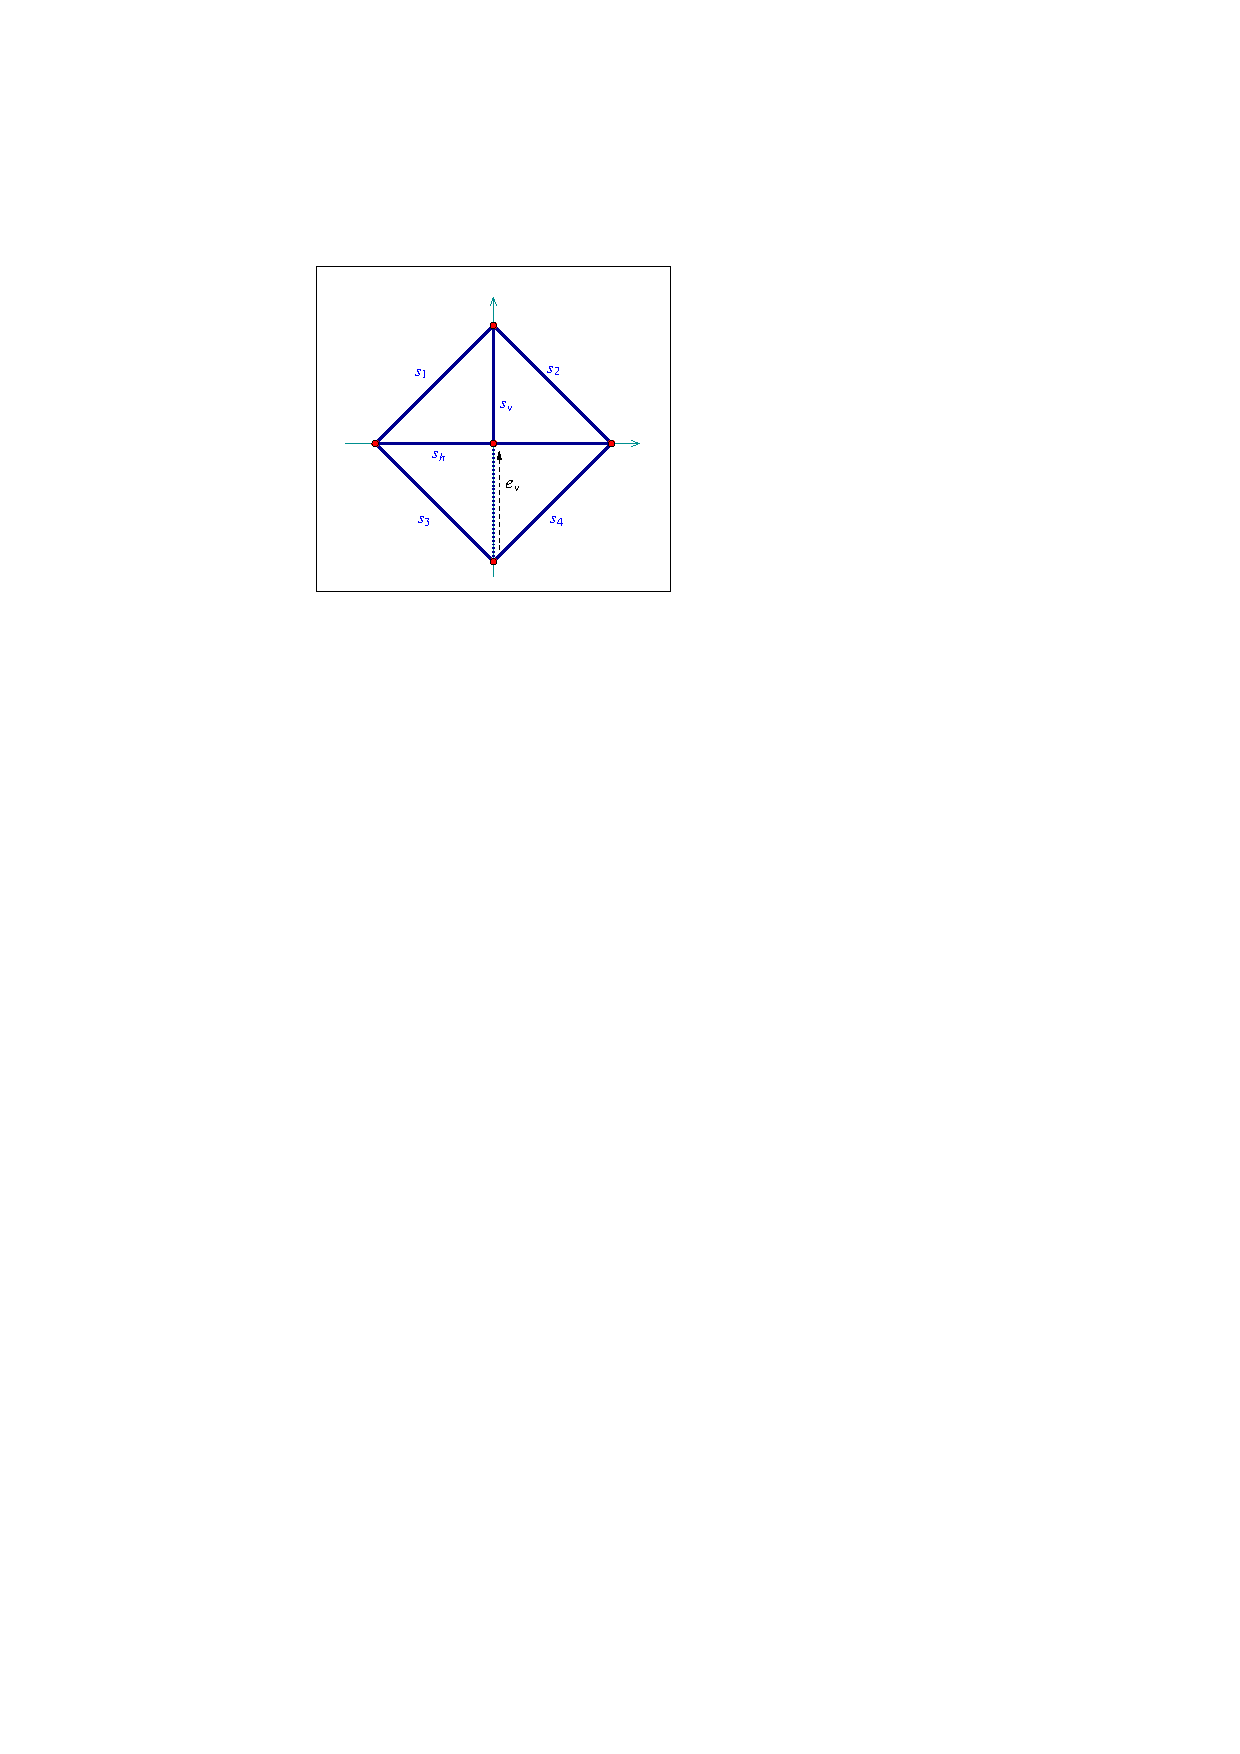
\includegraphics{Arrangement_2/fig/ex_19}
  \end{center}
\end{ccTexOnly}
\begin{ccHtmlOnly}
  <p><center>
  <img src="./fig/ex_19.gif" border=0 alt="Example 19">
  </center>
\end{ccHtmlOnly}
\caption{An arrangement of five line segments, as constructed in
\ccc{ex_observer.C}. The halfedge $e_v$ (dashed) is eventually
removed, so that the final arrangement consists of four faces (one
unbounded and three bounded ones).}
\label{arr_fig:ex_19}
\end{figure}

\begin{ccHtmlOnly}<p>\end{ccHtmlOnly}
The following example shows how to define and use an observer
class. The observer in the example keeps track of the arrangement
faces, and prints a message whenever a face is split into two due
to the insertion of an edge, and whenever two faces merge into one
due to the removal of an edge. The layout of the arrangement is
depicted in Figure~\ref{arr_fig:ex_19}:

\ccIncludeExampleCode{../examples/Arrangement_2/ex_observer.C}

\begin{ccHtmlOnly}<p>\end{ccHtmlOnly}
Observers are especially useful when the \dcel\ records are
extended and store additional data, as they help updating this
data on-line. See Section~\ref{arr_sec:ex_dcel} for more details
and examples.

\section{Extending the \dcel}
\label{arr_sec:ex_dcel}
%============================
%
For many applications of the arrangement package it is necessary to
store additional information (perhaps of non-geometric nature) with
the arrangement cells. As vertices are associated with \ccc{Point_2}
objects and edges (halfedge pairs) are associated with
\ccc{X_monotone_curve_2} objects, both defined by the traits class,
it is possible to extend the traits-class type by using a traits-class
decorator, as explained in Section~\ref{arr_ssec:meta_tr}, which may
be a sufficient solution for some applications.
However, the \dcel\ faces are not associated with any geometric object, 
so it is impossible to extend them using a traits-class decorator. 
Extending the \dcel\ face records comes handy is such caes. As a matter
of fact, it is possible to conveniently extend all \dcel\ records
(namely vertices, halfedges and faces), which can also be advantageous
for some applications.

\begin{ccHtmlOnly}<p>\end{ccHtmlOnly}
All examples presented so far use the default \ccc{Arr_default_dcel<Traits>}. 
This is done implicitly, as this class serves as a default parameter for 
the \ccc{Arrangement_2} template. The default \dcel\ class just associates 
points with vertices and $x$-monotone curves with halfedge, but nothing more. 
In this section we show how to use alternative \dcel\ types to extend the 
desired \dcel\ records.

\subsection{Extending the \dcel\ Faces}
\label{arr_ssec:ex_dcel_face}
%--------------------------------------
%
The \ccc{Arr_face_extended_dcel<Traits, FaceData>} class-template
is used to associate auxiliary data field of type \ccc{FaceData} to
each face record in the \dcel.

\begin{ccHtmlOnly}<p>\end{ccHtmlOnly}
When an \ccc{Arrangement_2} object is parameterized by this 
\dcel\ class, its nested \ccc{Face} type is extended with the access function
\ccc{data()} and with the modifier \ccc{set_data()}. Using these extra
functions it is straightforward to access and maintain the auxiliary
face-data field.

\begin{ccHtmlOnly}<p>\end{ccHtmlOnly}
Note that the extra data fields must be maintained by the application
programmers. They may choose to construct their arrangement, and
only then go over the faces and attach the appropriate data fields to
the arrangement faces. However, in some cases the face data can only
be computed when the face is created (split from another face, or merged
with another face). In such cases one can use an arrangement observer
tailored for this task, which receives updates whenever a face is
modified and sets its data field accordingly.

\begin{figure}[!htp]
\begin{ccTexOnly}
  \begin{center}
  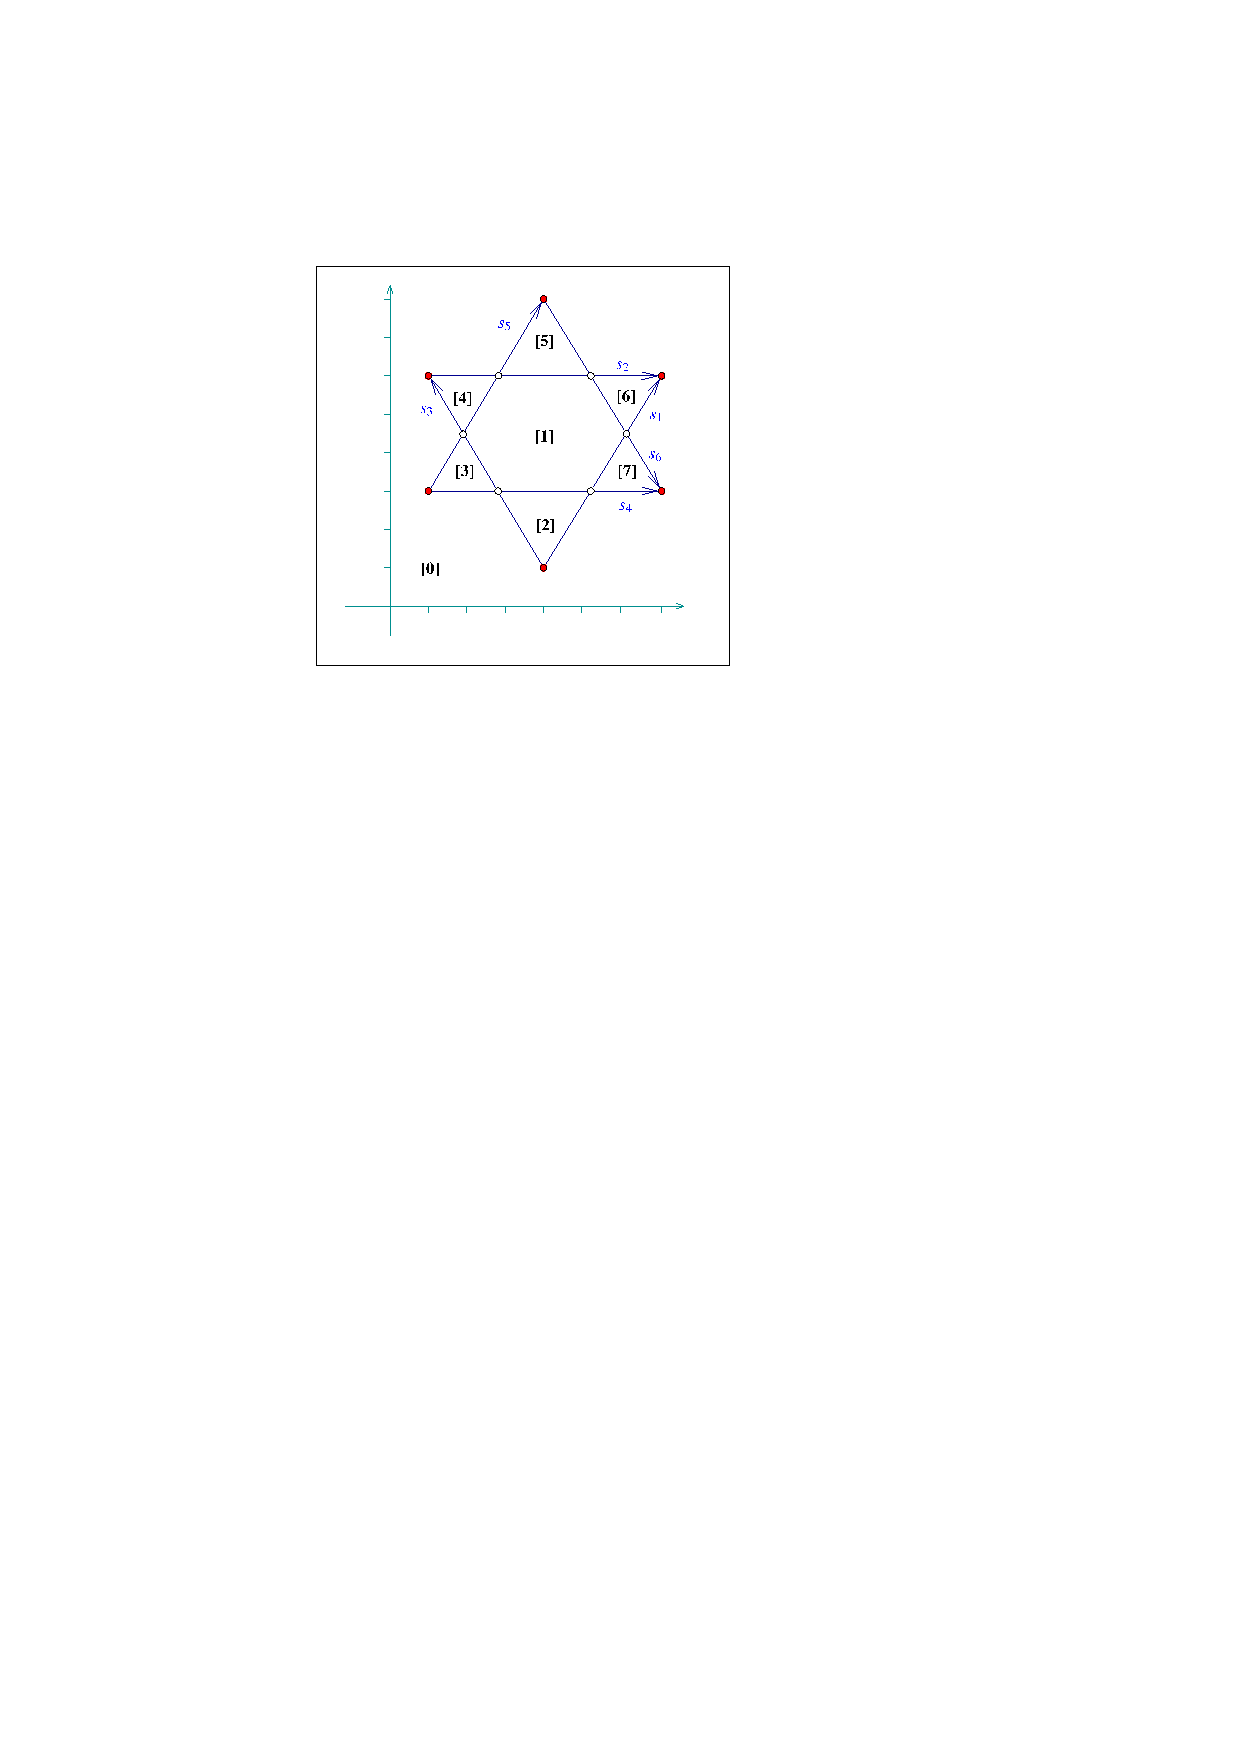
\includegraphics{Arrangement_2/fig/ex_20}
  \end{center}
\end{ccTexOnly}
\begin{ccHtmlOnly}
  <p><center>
  <img src="./fig/ex_20.gif" border=0 alt="Example 20">
  </center>
\end{ccHtmlOnly}
\caption{An arrangement of six line segments, as constructed in
\ccc{ex_face_extension.C} and \ccc{ex_dcel_extension.C}
(in \ccc{ex_dcel_extension.C} we treat
the segments as directed, so they are drawn as arrows directed from the
source to the target). The indices associated with the halfedges in
\ccc{ex_face_extension.C} are shown in brackets.}
\label{arr_fig:ex_20}
\end{figure}

\begin{ccHtmlOnly}<p>\end{ccHtmlOnly}
The next example constructs an arrangement that contains seven bounded 
faces induced by six line segments (see Figure~\ref{arr_fig:ex_20}). An 
observer gets notified each time a new face $f$ is created and it associates 
$f$ with a running index, (where the index of the unbounded face
is 0). As a result, the faces are numbered according to their creation
order, as one can easily verify by examining the insertion order of the
segments:\footnote{For simplicity, the particular observer used must be
attached to an empty arrangement. It is not difficult however to modify 
the program to handle the general case of attaching a similar observer
to a non-empty arrangement.}

\ccIncludeExampleCode{../examples/Arrangement_2/ex_face_extension.C}

\subsection{Extending All \dcel\ Records}
\label{arr_ssec:ex_dcel_all}
%----------------------------------------
%
The \ccc{Arr_extended_dcel<Traits, VertexData, HalfedgeData, FaceData>}
class-template is used to associate auxiliary data fields of
types \ccc{VertexData} \ccc{HalfedgeData}, and \ccc{FaceData} to
each \dcel\ vertex, halfedge, and face record types, respectively.

\begin{ccHtmlOnly}<p>\end{ccHtmlOnly}
When an \ccc{Arrangement_2} object is injected with this
\dcel\ class, each one of its nested \ccc{Vertex}, \ccc{Halfedge} and
\ccc{Face} classes is extended by the access function \ccc{data()}
and by the modifier \ccc{set_data()}.

\begin{ccHtmlOnly}<p>\end{ccHtmlOnly}
The next example shows how to use a \dcel\ with extended vertex,
halfedge, and face records. In this example each vertex is associated 
with a color, which may be blue, red, or white, depending on whether the
vertex is isolated, represents a segment endpoint, or whether it
represents an intersection point. Each halfedge is associated with
Boolean flag indicating whether its direction is the same as the
direction of its associated segment (in this example segments are
treated as directed objects). Each face is also extended to store the
size of its outer boundary.

\begin{ccHtmlOnly}<p>\end{ccHtmlOnly}
The constructed arrangement, depicted in Figure~\ref{arr_fig:ex_20}, is 
similar to the arrangement constructed in the previous example. 
Note that all auxiliary data fields are set during the construction phase.
Also note that the data fields are properly maintained when the arrangement
is copied to another arrangement instance:
 
\ccIncludeExampleCode{../examples/Arrangement_2/ex_dcel_extension.C}

\section{Overlaying Arrangements}
\label{arr_sec:overlay}
%================================
%
Assume that we are given two geographic maps, represented as
arrangements with some data objects attached to their faces,
representing some geographic information --- for example, a map of
the annual precipitation in some country and a map of the vegetation
in the same country. It is interesting to overlay the two maps to
locate, for example, the regions where there is a pine forest and
the annual precipitation is between 1000\,mm and 1500\,mm. 

\begin{ccHtmlOnly}<p>\end{ccHtmlOnly}
Computing the overlay of two planar arrangement is also useful for
supporting Boolean set operations on polygons (or generalized polygons,
see, e.g.,~\cite{behsms-cbcab-02}).

\begin{ccHtmlOnly}<p>\end{ccHtmlOnly}
The function \ccc{overlay (arr_a, arr_b, ovl_arr, ovl_traits)} accepts
two input arrangement instances \ccc{arr_a} and \ccc{arr_b}, and constructs
their overlay instance \ccc{ovl_arr}. All three arrangements must use the
same geometric primitives. In other words, their types must be defined 
using the same geometric traits-class. Let us assume that \ccc{arr_a} is of 
type \ccc{Arrangement_2<Traits,Dcel_A>}, \ccc{arr_b} is of type
\ccc{Arrangement_2<Traits,Dcel_B>} and the resulting \ccc{ovl_arr} is of type 
\ccc{Arrangement_2<Traits,Dcel_R>}. The \ccc{ovl_traits} parameter is
an instance of an {\em overlay traits-class}, which enables the creation of
\ccc{Dcel_R} records in the overlaid arrangement from the \dcel\ features
of \ccc{arr_a} and \ccc{arr_b} that they correspond to.

\begin{ccHtmlOnly}<p>\end{ccHtmlOnly}
In principle, we distinguish between three levels of overlay:
\begin{description}
\item[Simple overlay:]
An overlay of two arrangements that store no additional data
with their \dcel\ records. That is, they are defined using the default 
\dcel\ class \ccc{Arr_default_dcel}. Typically, the overlaid
arrangement in this case stores no extra data with its \dcel\ records as
well (or if it does, the additional data fields cannot be computed by
the overlay operation), so by overlaying the two arrangement we just
compute the arrangement of all curves that induce \ccc{arr_a} and \ccc{arr_b}.
Note that the same result can be obtained using the standard insertion
operations, but users may choose to use overlay computation in order to
achieve better running times.

\begin{ccHtmlOnly}<p>\end{ccHtmlOnly}
The \ccc{Arr_default_overlay_traits} class should be used as an overlay
traits-class for such simple overlay operations.
%
\item[Face overlay:]
An overlay of two arrangements that store additional data
fields with their faces (e.g., the geographic-map example
given in the beginning of this section). The resulting overlaid arrangement
typically also stores extraneous data fields with its faces, where the
data field that is attached to an overlaid face can be computed from the
data fields of the two faces (in \ccc{arr_a} and \ccc{arr_b}) that induce
the overlaid face.

\begin{ccHtmlOnly}<p>\end{ccHtmlOnly}
The \ccc{Arr_face_overlay_traits} class should be used as an overlay
traits-class for face-overlay operations. It operates on arrangement, whose
\dcel\ representation is based on the \ccc{Arr_face_extended_dcel}
class-template (see Section~\ref{arr_ssec:ex_dcel_face}). The face-overlay
traits-class is parameterized by a functor that is capable of combining two
face-data fields of types \ccc{Dcel_A::Face_data} and
\ccc{Dcel_B::Face_data}, and computing the output \ccc{Dcel_R::Face_data}
object. The overlay traits-class uses this functor to properly construct
the overlaid faces.
%
\item[Full overlay:]
An overlay of two arrangements that store additional data
fields with all their \dcel\ records. That is, their \dcel\ classes
are instantiations of the \ccc{Arr_extended_dcel} class-template (see
Section~\ref{arr_ssec:ex_dcel_all}), where the resulting arrangement
also extends it \dcel\ records with data fields computed on the basis
of the overlapping \dcel\ features of the two input arrangements.
\end{description}

\begin{ccHtmlOnly}<p>\end{ccHtmlOnly}
In the following subsections we give some examples for the simple and the
face-overlay operations and demonstrate how to use the auxiliary overlay
traits-classes. For the full overlay operations users need to implement
their specialized overlay traits-class, which models the \ccc{OverlayTraits}
concept. The details of this concept are given in the reference manual.

\subsection{Example for a Simple Overlay}
\label{arr_ssec:simp_ovl}
%----------------------------------------
%
\begin{figure}[!htp]
\begin{ccTexOnly}
  \begin{center}
  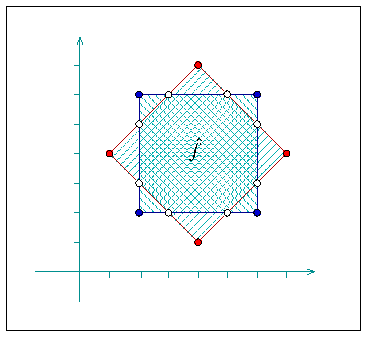
\includegraphics{Arrangement_2/fig/ex_22}
  \end{center}
\end{ccTexOnly}
\begin{ccHtmlOnly}
  <p><center>
  <img src="./fig/ex_22.gif" border=0 alt="Example 22">
  </center>
\end{ccHtmlOnly}
\caption{Overlaying two simple arrangements of line segments, as done
in \ccc{ex_overlay.C} and \ccc{ex_face_extension_overlay.C}.
In \ccc{ex_face_extension_overlay.C} we concider
the two bounded faces as {\em marked}, were the intersection of the two
marked faces is denoted as $\hat{f}$.}
\label{arr_fig:ex_22}
\end{figure}

\begin{ccHtmlOnly}<p>\end{ccHtmlOnly}
The next program constructs two simple arrangements, as depicted in
Figure~\ref{arr_fig:ex_22} and computes their overlay:

\ccIncludeExampleCode{../examples/Arrangement_2/ex_overlay.C}

\subsection{Example for a Face Overlay}
\label{arr_ssec:face_ovl}
%--------------------------------------
%
The following example shows how to compute the intersection of two polygons
using the \ccc{overlay()} function. It uses a face-extended \dcel\ class
to define our arrangement class. The \dcel\ extends each face with a Boolean 
flag. A polygon is represented as a {\sl marked} arrangement face, (whose
flag is set). The example uses a face-overlay traits class, instanciated with 
a functor that simply performs a logical {\em and} operations on Boolean flags.
As a result, a face in the overlaid arrangement is marked only, when it
corresponds to an overlapping region of two marked cells in the input
arrangements. Namely, it is part of the intersection of the two polygons.

\begin{ccHtmlOnly}<p>\end{ccHtmlOnly}
The example computes the intersection between a square and a rhombus, (which is
actually also a square). The resulting polygon is an octagon, represented 
by the shape $\hat{f}$ in Figure~\ref{arr_fig:ex_22}:

\ccIncludeExampleCode{../examples/Arrangement_2/ex_face_extension_overlay.C}

\section{Storing the Curve History}
\label{arr_sec:arr_with_hist}
%==================================
%
As states at the beginning of this chapter (see Section~\ref{arr_sec:intro}), 
when one constructs an arrangement induced by a set $\calC$ of arbitrary 
planar curves, she or he constructs a collection $\calC''$ of $x$-monotone 
subcurves of $\calC$ that are pairwise disjoint in their interior, and these 
subcurves are associated with the arrangement edges (more precisely, with the 
\dcel\ halfedges). Doing so, the connection between the originating input 
curves and the arrangement edges is lost. This loss might be acceptable for 
some applications. However, in many practical cases it is important to 
determine the input curves that originate final subcurves.

\begin{ccHtmlOnly}<p>\end{ccHtmlOnly}
The \ccc{Arrangement_with_history_2<Traits,Dcel>} class-template extends
the \ccc{Arrangement_2} class by keeping an additional container of input
curves representing $\calC$, and by maintaining a cross-mapping between these
curves and the arrangement edges they induce. The traits class that is
used for instantiating the template should be a model of the
\ccc{ArrangementTraits_2} concept (see Section~\ref{arr_sssec:insert_gen}).
That is, it should define the \ccc{Curve_2} type (and not just the
\ccc{X_monotone_curve_2} type). The \ccc{Dcel} parameter should model the 
\ccc{ArrangementDcel} concept. Users can use the default \dcel\ class or 
an extended \dcel\ class according to their needs.

\subsection{Traversing an Arrangement with History}
\label{arr_ssec:arrwh_traverse}
%--------------------------------------------------
%
The \ccc{Arrangement_with_history_2} class extends the \ccc{Arrangement_2}
class, thus all the iterator and circulator types that are defined by the
arrangement class are also available in \ccc{Arrangement_with_history_2}.
The reader is referred to Section~\ref{arr_ssec:traverse} for a comprehensive
review of these functions.

\begin{ccHtmlOnly}<p>\end{ccHtmlOnly}
As mentioned above, the \ccc{Arrangement_with_history_2} class maintains
a container of input curves, which can be accessed using curve handles.
The member function \ccc{number_of_curves()} returns the number of input 
curves stored in the container, while \ccc{curves_begin()} and 
\ccc{curves_end()} return \ccc{Arrangement_with_history_2::Curve_iterator}
objects that define the  valid range of curves that induce the arrangement.
The value type of this iterator is \ccc{Curve_2}. Moreover, the curve-iterator
type is equivalent to  \ccc{Arrangement_with_history_2::Curve_handle}, which
is used for accessing the stored curves. Conveniently, the corresponding
constant-iterator and constant-handle types are also defined.

\begin{ccHtmlOnly}<p>\end{ccHtmlOnly}
As mentioned in the previous paragraph, a \ccc{Curve_handle} object \ccc{ch} 
serves as a pointer to a curve stored in an arrangement-with-history instance 
\ccc{arr}. Using this handle, it is possible to obtain the number of 
arrangement edges this curve induces by calling 
\ccc{arr.number_of_induced_edges(ch)}. The functions 
\ccc{arr.induced_edges_begin(ch)} and
\ccc{arr.induced_edges_end(ch)} return iterators of type
\ccc{Arrangement_with_history_2::Induced_edges_iterator} that define the
valid range of edges induced by \ccc{ch}. The value type of these iterators
is \ccc{Halfedge_handle}. It is thus possible to traverse all arrangement
edges induced by an input curve.

\begin{ccHtmlOnly}<p>\end{ccHtmlOnly}
It is also important to be able to perform the inverse mapping: given an
arrangement edge, we would like to be able to determine which input curve
induces it. In case the edge represents an overlap of several curves, we
should be able to trace all input curves that overlap over this edge.
The \ccc{Arrangement_with_history_2} class is extended by several member
functions that enable such an inverse mapping. Given a halfedge handle \ccc{e}
in an arrangement with history \ccc{arr}, then 
\ccc{arr.number_of_originating_curves(e)} returns the number of curves that
induce the edge (which should be 1 in non-degenerate cases, and 2 or more
in case of overlaps), while \ccc{arr.originating_curves_begin(e)} and 
\ccc{arr.originating_curves_end(e)} return 
\ccc{Arrangement_with_history_2::Originating_curve_iterator} objects that
define the range of curves that induce \ccc{e}. The value type of these
iterator is of course \ccc{Arrangement_with_history_2::Curve_with_edges_2}.

\begin{ccHtmlOnly}<p>\end{ccHtmlOnly}
In this context we mention that it is possible to overlay two 
arrangement-with-history instances that are templated by the same traits
class. In this case, the resulting arrangement will store a consolidated
container of input curves and automatically preserve the cross-mapping
between the arrangement edges and the consolidated curve set. Needless to
say, users can employ and overlay-traits class to maintain any type of
auxiliary data kept with the \dcel\ features (see 
Section~\ref{arr_sec:overlay}).

\subsection{Modifying an Arrangement with History}
\label{arr_ssec:modif_traverse}
%-------------------------------------------------
%
As the \ccc{Arrangement_with_history_2} class extends the \ccc{Arrangement_2}
class, it inherits the fundamental modification operations, such as 
\ccc{assign()} and \ccc{clear()}, from it. The vertex-manipulation functions
are also inherited and supported (see Sections~\ref{arr_sssec:mf_iso_verts}
and~\ref{arr_sssec:insert_point} for the details). However, there are some 
fundamental differences between the interfaces of the two classes, which we
highlight in this subsection.

\begin{ccHtmlOnly}<p>\end{ccHtmlOnly}
The most significant difference between the arrangement-with-history class
and the basic arrangement class is the way they handle their input curves.
\ccc{Arrangement_with_history_2} always stores the \ccc{Curve_2} objects
that induce it, thus it is impossible to insert $x$-monotone curves into
an arrangement with history. The free \ccc{insert_non_intersecting_curve()}
and \ccc{insert_x_monotone_curve()} (as well as their aggregated versions)
are therefore not available for arrangement-with-history instances
and only the free \ccc{insert_curve()} and \ccc{insert_curves()} functions
(the incremental insertion function and the aggregated insertion function)
are supported --- see also Section~\ref{arr_sssec:insert_gen}. Notice however
that while the incremental insertion function \ccc{insert_curve(arr,c)} for
an \ccc{Arrangement_2} object \ccc{arr} does not have a return value,
the corresponding arrangement-with-history function returns a
\ccc{Curve_handle} to the inserted curve.

\begin{ccHtmlOnly}<p>\end{ccHtmlOnly}
As we are able to keep track of all edges induced by an input curve, we also
provide a free function that removes a curve from an arrangement. By calling
\ccc{remove(arr,ch)}, where \ccc{ch} is a valid curve handle, the given curve
is deleted from the curve container, and all its edges induced solely by
this curve (i.e., excluding overlapping edges) are removed from the 
arrangement. The function returns the number of edges that have been removed.

\begin{ccHtmlOnly}<p>\end{ccHtmlOnly}
In some cases, users may need to operate directly on the arrangement edges.
We first mention that the specialized insertion functions (see 
Section~\ref{arr_sssec:mf_insert_cv}) are not supported, as they accept
$x$-monotone curves. Insertion can only be performed via the free 
insertion-functions. The other edge-manipulation functions 
(see Section~\ref{arr_sssec:mf_halfedges}) are however available, but have 
a different interface that does not use $x$-monotone curves:
\begin{itemize}
\item Invoking \ccc{split_edge(e,p)} splits the edge \ccc{e} at a given point
\ccc{p} that lies in its interior.
\item Invoking \ccc{merge_edge(e1,e2)} merges the two given edges. There is
a precondition that \ccc{e1} and \ccc{e2} shared a common end-vertex of degree
2, and that the $x$-monotone subcurves associated with these edges are
mergeable.
\item It is possible to remove an edge by simply invoking
\ccc{remove_edge(e)}.
\end{itemize}
In all cases, the maintenance of cross-pointers for appropriate input
curves will be done automatically.

\begin{ccHtmlOnly}<p>\end{ccHtmlOnly}
It should be noted that it is possible to attach observers to an 
arrangement-with-history instance in order to get detailed notifications of
the changes the arrangements undergoes (see Section~\ref{arr_sec:notif} for
the details).

\subsection{Examples}
\label{arr_ssec:arr_hist_ex}
%---------------------------
%
\begin{figure}[!htp]
\begin{ccTexOnly}
  \begin{center}
  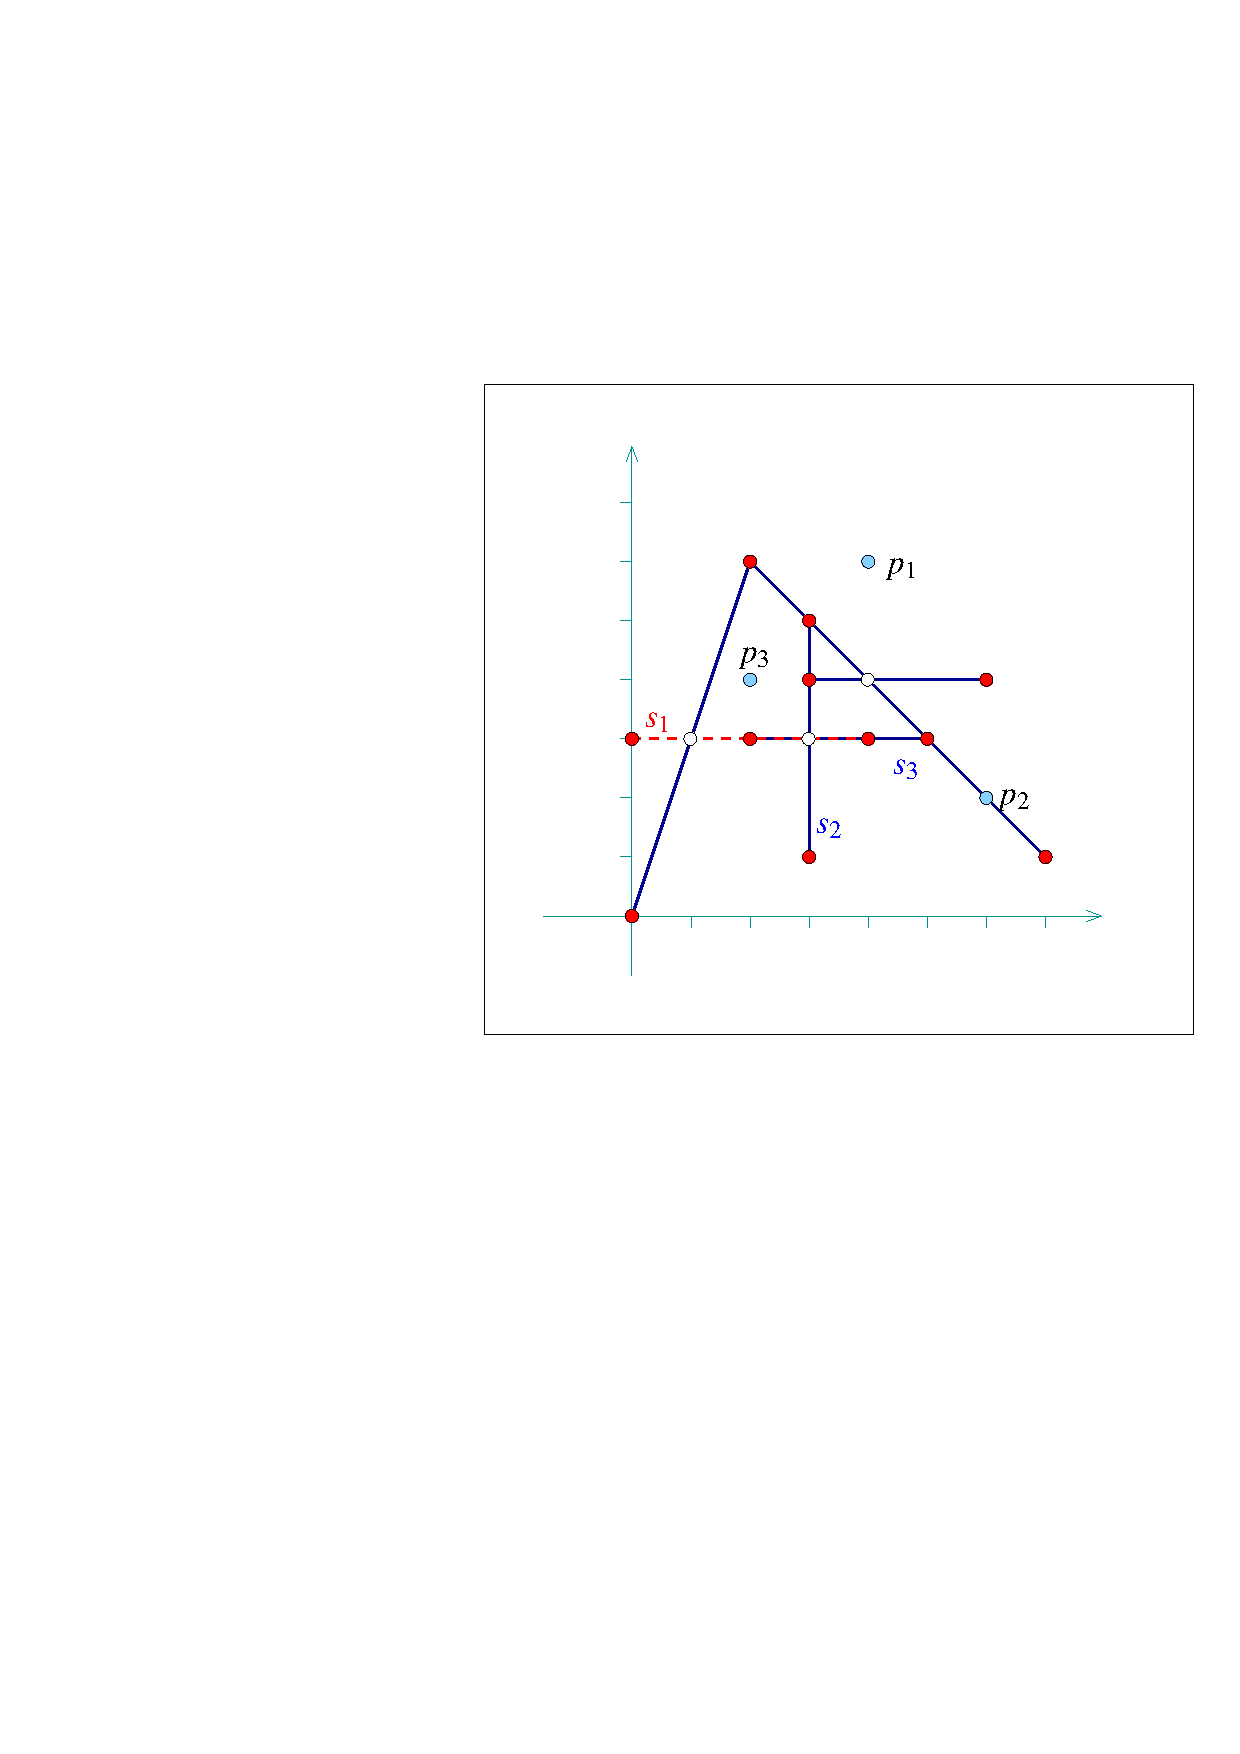
\includegraphics{Arrangement_2/fig/ex_24}
  \end{center}
\end{ccTexOnly}
\begin{ccHtmlOnly}
  <p><center>
  <img src="./fig/ex_24.gif" border=0 alt="Example 24">
  </center>
\end{ccHtmlOnly}
\caption{An arrangement with history as constructed in
\ccc{ex_curve_history.C}. 
Note that $s_1$ and $s_3$ overlap over two edges. The point-location query
points are drawn as lightly shaded dots.}
\label{arr_fig:ex_24}
\end{figure}

\begin{ccHtmlOnly}<p>\end{ccHtmlOnly}
In the following example we construct a simple arrangement of six line
segments, as depicted in Figure~\ref{arr_fig:ex_24}, while maintaining 
the curve history. The example demonstrates the usage of the special
traversal functions. It also shows how to issue point-location queries
on the resulting arrangement:

\ccIncludeExampleCode{../examples/Arrangement_2/ex_curve_history.C}

\begin{figure}[!htp]
\begin{ccTexOnly}
  \begin{center}
  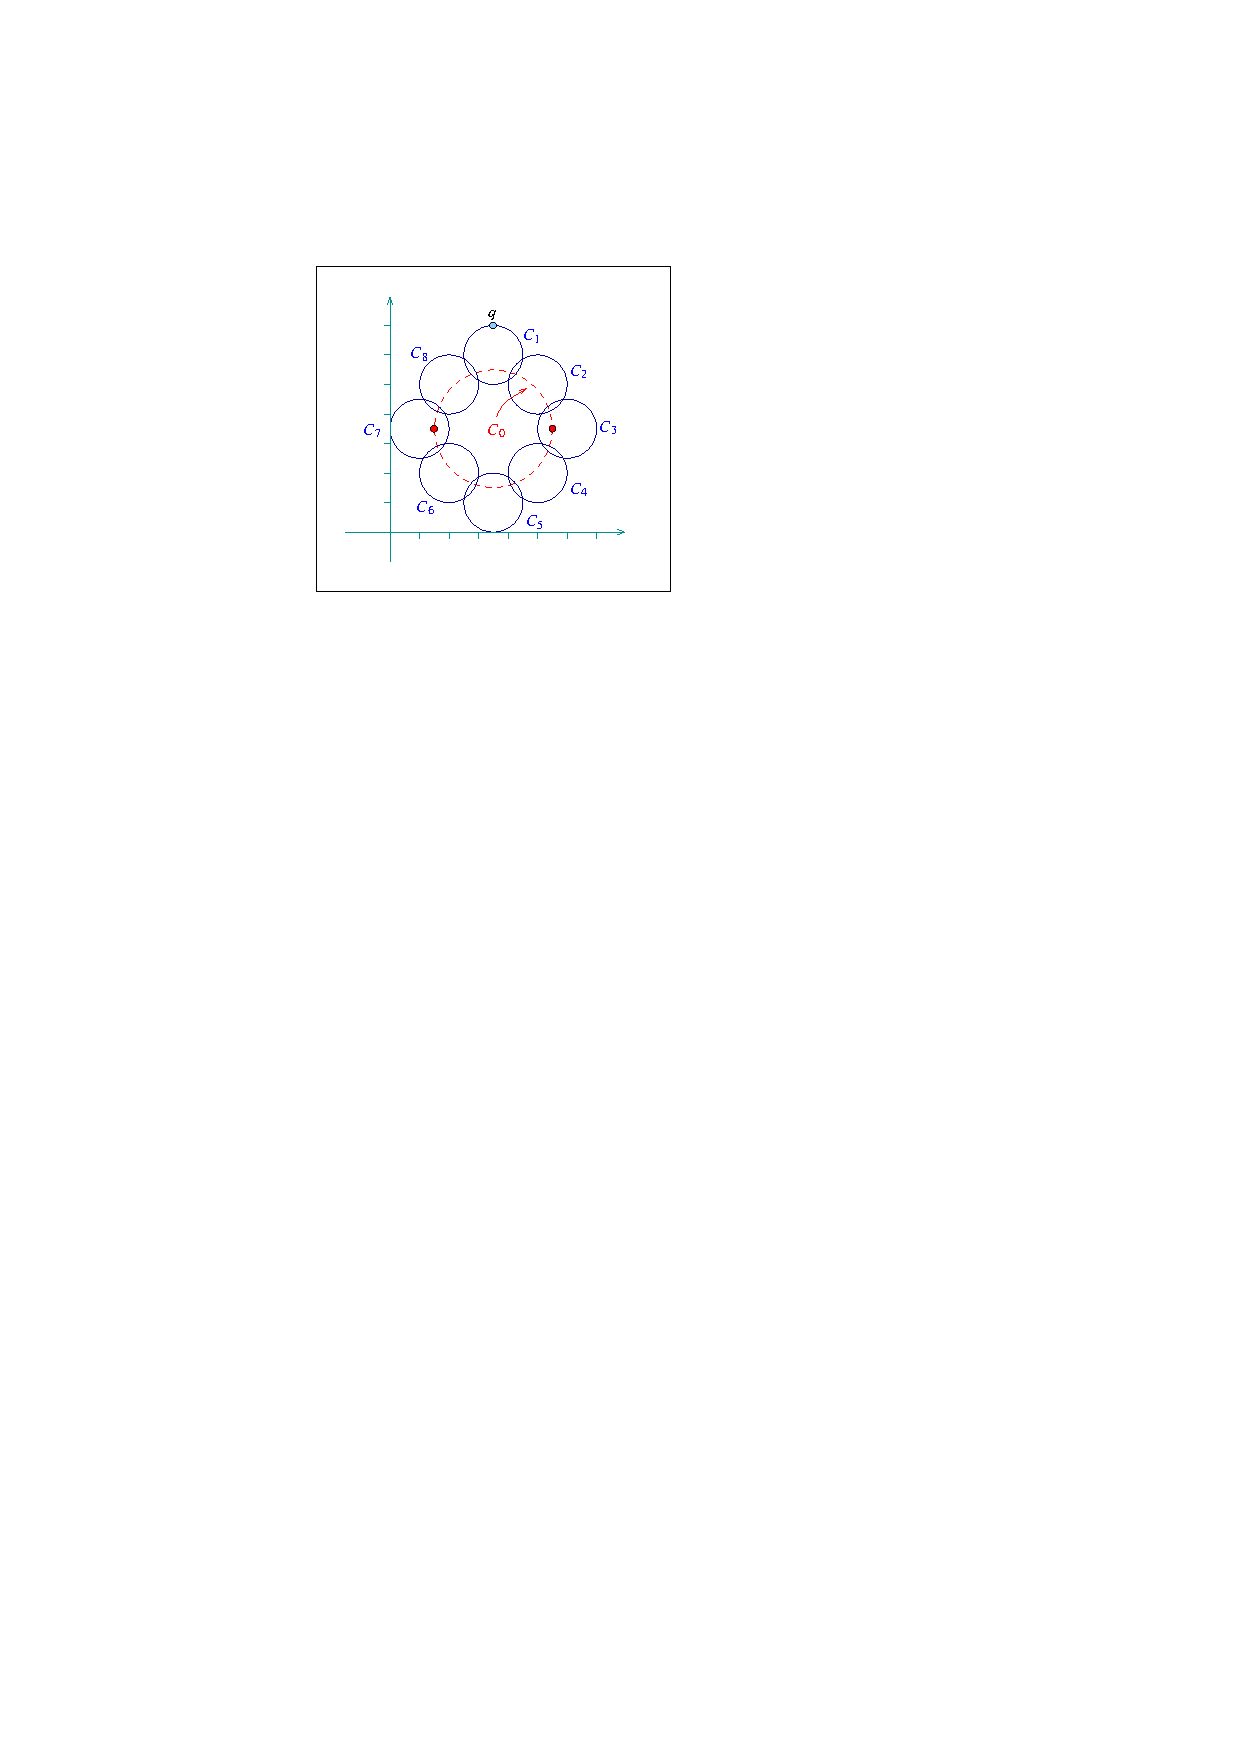
\includegraphics{Arrangement_2/fig/ex_25}
  \end{center}
\end{ccTexOnly}
\begin{ccHtmlOnly}
  <p><center>
  <img src="./fig/ex_25.gif" border=0 alt="Example 25">
  </center>
\end{ccHtmlOnly}
\caption{An arrangement with history of nine circle as constructed in 
\ccc{ex_edge_manipulation_curve_history.C}. The large circle $C_0$ is
eventually removed from the arrangement, with all 18 edges it induces.}
\label{arr_fig:ex_25}
\end{figure}

\begin{ccHtmlOnly}<p>\end{ccHtmlOnly}
The following example demonstrates the usage of the free \ccc{remove()}
function. We construct an arrangement of nine circles, while keeping a handle
to each inserted circle. We then remove the large circle $C_0$, which induces
$18$ halfedges, as depicted in Figure~\ref{arr_fig:ex_25} (note the 
vertical tangency points that are marked as red dots). The example also shows
how to use the \ccc{split_edge()} and \ccc{merge_edge()} functions when
operating on an arrangement-with-history instance:

\ccIncludeExampleCode{../examples/Arrangement_2/ex_edge_manipulation_curve_history.C}

\section{Input/Output Functions}
\label{arr_sec:io}
%===============================
%
In some cases, we would like to reuse an arrangement instance constructed
by our application in the future --- for example, our arrangement may
represent a very complicated geographical map and we have various
applications that need to answer point-location queries on this map.
Naturally, we can store the set of curves that induces the arrangement,
but this implies that we need to construct the arrangement from
scratch each time we need to reuse it. A more efficient solution would
be to save the arrangement to a file, so that other application can
reread it from there.

\begin{ccHtmlOnly}<p>\end{ccHtmlOnly}
We provide an {\em inserter} (the \ccc{<<} operator) and an {\em extractor}
(the \ccc{>>} operator) for the \ccc{Arrangement_2<Traits,Dcel>} class,
such that an arrangement instance can be inserted into an output stream
or read from an input stream. The arrangement is written using a simple
predefined textual format that encodes the arrangement topology, as
well as all geometric entities associated with vertices and edges.

\begin{ccHtmlOnly}<p>\end{ccHtmlOnly}
To use the input/output operators, we require that the \ccc{Point_2} type
and the \ccc{X_monotone_curve_2} type defined by the traits class both
support the \ccc{<<} and\ccc{>>} operators. The \ccc{Arr_conic_traits_2}
class (see Section~\ref{arr_ssec:tr_conic}) and the 
\ccc{Arr_rational_arc_traits_2} class (see Section~\ref{arr_ssec:tr_ratfunc})
currently do not provide these operator for the geometric types
they define, so only arrangements of line segments or of polylines can
be written or read.

\begin{ccHtmlOnly}<p>\end{ccHtmlOnly}
The following example constructs the arrangement depicted in 
Figure~\ref{arr_fig:ex_5} and writes it to an output file. It also
demonstrates how to re-read the arrangement from a file:

\ccIncludeExampleCode{../examples/Arrangement_2/ex_io.C}

\begin{ccAdvanced}
\subsection{Arrangements with Auxiliary Data}
\label{arr_ssec:arr_io_aux_data}
%--------------------------------------------
%
The inserter and extractor both ignore any auxiliary data stored with
the arrangement features, thus they are ideal for arrangements
instantiated using the \ccc{Arr_default_dcel} class.
However, as explained in Section~\ref{arr_sec:ex_dcel}, one can easily
extend the arrangement faces by using the \ccc{Arr_face_extended_dcel}
template, or extend all \dcel\ records by using the \ccc{Arr_extended_dcel}
template. In such cases, it may be crucial that the auxiliary data fields
are written to the file or read from there.

\begin{ccHtmlOnly}<p>\end{ccHtmlOnly}
The arrangement package includes the free functions
\ccc{write(arr, os, formatter)}, which writes the arrangement \ccc{arr}
to an output stream \ccc{os}, and \ccc{read(arr, os, formatter)}, which
reads the arrangement \ccc{arr} from an input stream \ccc{is}. Both
operations are performed using a \ccc{formatter} object, which define
the I/O format. The package contains three formatter classes:
\begin{itemize}
\item \ccc{Arr_text_formatter<Arrangement>} defines a simple textual
I/O format for the arrangement topology and geometry, disregarding any
auxiliary data that may be associated with the arrangement features.
This is the default formatter used by the arrangement inserter and the
arrangement extractor, as defined above.
%
\item \ccc{Arr_face_extended_text_formatter<Arrangement>} operates on
arrangements whose \dcel\ representation is based on the
\ccc{Arr_face_extended_dcel<Traits,FaceData>} class (see
Section~\ref{arr_ssec:ex_dcel_face}). It supports reading and writing
the auxiliary data objects stored with the arrangement faces providing
that the \ccc{FaceData} class supports an inserter and an extractor.
%
\item \ccc{Arr_extended_dcel_text_formatter<Arrangement>} operates on
arrangements whose \dcel\ representation is based on the
\ccc{Arr_extended_dcel<Traits,VertexData,HalfedgeData,FaceData>} class
(see Section~\ref{arr_ssec:ex_dcel_all}). It supports reading and writing
the auxiliary data objects stored with the arrangement vertices, edges
and faces, providing that the \ccc{VertexData}, \ccc{HalfedgeData} and
\ccc{FaceData} classed all have inserters and extractors.
\end{itemize}

\begin{ccHtmlOnly}<p>\end{ccHtmlOnly}
The following example constructs the same arrangement as the
example \ccc{ex_dcel_extension} does
(see Section~\ref{arr_ssec:ex_dcel_all}) which is depicted in
Figure~\ref{arr_fig:ex_20}, and writes it to an output file. It also
demonstrates how to re-read the arrangement from a file:

\ccIncludeExampleCode{../examples/Arrangement_2/ex_dcel_extension_io.C}

\begin{ccHtmlOnly}<p>\end{ccHtmlOnly}
External users may write their own formatter classes by implementing
models to the \ccc{ArrangementInputFormatter} and the
\ccc{ArrangementOutputFormatter}, as defined in the reference manual.
Doing so, they can define other I/O formats, such as an XML-based
format or a binary format.
\end{ccAdvanced}

\subsection{Arrangements with Curve History}
\label{arr_ssec:arr_io_hist}
%-------------------------------------------
%
In Section~\ref{arr_sec:arr_with_hist} we introduced the
\ccc{Arrangement_with_history_2<Traits,Dcel>} class that stores the
set of curves inducing the arrangement and maintains the relations between
these curves and the edges they induce. Naturally, when reading or writing an
arrangement-with-history instance we would like this information to be
written to the output stream or retrieved from the input stream alongside
with the basic arrangement structure.

\begin{ccHtmlOnly}<p>\end{ccHtmlOnly}
The arrangement package supplies an inserter and an extractor for the
\ccc{Arrangement_with_history_2<Traits,Dcel>} class. The arrangement is
represented using a simple predefined textual format, where we require that
the \ccc{Curve_2} type defined by the traits class (as well as the
\ccc{Point_2} type and the \ccc{X_monotone_curve_2} types) supports
the \ccc{<<} and\ccc{>>} operators.

\begin{ccHtmlOnly}<p>\end{ccHtmlOnly}
The following example constructs the same arrangement as example
\ccc{ex_curve_history} does
(see Section~\ref{arr_ssec:arr_ssec:arr_hist_ex}) which is depicted in
Figure~\ref{arr_fig:ex_24}, and writes it to an output file. It also
demonstrates how to re-read the arrangement-with-history from a file:

\ccIncludeExampleCode{../examples/Arrangement_2/ex_io_curve_history.C}

\begin{ccAdvanced}
The arrangement package also includes the free functions
\ccc{write(arr, os, formatter)} and \ccc{read(arr, os, formatter)} that
operate on a given arrangement-with-history instance \ccc{arr}.
Both functions are templated by a \ccc{formatter} object, which define
the I/O format. The package contains a template called,
\ccc{Arr_with_hist_text_formatter<ArranagmentFormatter>}, which extends
an arrangement formatter class (see Section~\ref{arr_ssec:arr_io_aux_data})
and defines a simple textual input/output format.
\end{ccAdvanced}

\section{Adapting to {\sc Boost} Graphs}
\label{arr_sec:bgl}
%=======================================
%
\boost\ is a collection of portable \Cpp\ libraries that work well with,
and are in the same spirit as, the Standard Template Library. The
\boost\ Graph Library (BGL), one of the libraries in the collection,
offers an extensive set of generic graph algorithms parameterized through
templates. As our arrangements are embedded as planar graphs, it is only 
natural to extend the undelying data structure with the interface that the 
BGL expects, and gain the ability to perform the operations that the BGL 
supports, such as shortest-path computation. This sections describes how to 
adapt \ccc{Arrangement_2} to BGL graphs, so that an \ccc{Arrangement_2}
instance can be passed as input to a generic algorithm already implemented 
in the BGL. Thus, enabling the use of BGL algorithms instantly. (For more 
information about \boost, visit {\tt www.boost.org}).

An instance of \ccc{Arrangement_2} is adapted to a \boost\ graph through the
provision of a set of free functions that operate on the arrangement features
and conform with the relevant BGL concepts. Besides the straightforward 
adaptation, which associates a vertex with each \dcel\ vertex and an edge 
with each \dcel\ halfedge, the package also offer a {\em dual} adaptor, which 
associates a graph vertex with each \dcel\ face, such that two vertices are 
connected, iff there is a \dcel\ halfedge that connects the two corresponding
faces. 

\begin{ccHtmlOnly}<p>\end{ccHtmlOnly}
The class templates \ccc{Arr_bgl_adaptor<Arrangement>} and
\ccc{Arr_bgl_dual_adaptor<Arrangement>} adapt \ccc{Arrangement_2} to BGL 
graphs, when instanciated with \ccc{Arrangement_2}. An instance of any one
these two types models the \ccc{Graph}, \ccc{IncidenceGraph}, and 
\ccc{VertexListGraph} \boost\ concepts. It defines the necessary types and 
methods required by these concepts. The \ccc{Arr_bgl_adaptor} adaptor 
considers the \ccc{Arrangement_2} vertices as the vertices of the BGL graph. 
More precisely, \ccc{Arrangement_2::Vertex_handle} is the graph-vertex type,
and \ccc{Arrangement_2::Halfedge_handle} is the graph-edge type. 
The \ccc{Arr_bgl_dual_adaptor}, on the other hand, considers the 
\ccc{Arrangement_2} faces as the vertices of the BGL graph. More precisely, 
\ccc{Arrangement_2::Face_handle} is the graph-vertex type.
(\ccc{Arrangement_2::Halfedge_handle} is the graph-edge type as above.)
We can use the the \ccc{make_arr_bgl_adaptor(Arrangement & arr)} and
\ccc{make_arr_bgl_dual_adaptor(Arrangement & arr)} function templates
to conveniently generate an appropriate adapted arrangement out of a given 
one.

\begin{ccHtmlOnly}<p>\end{ccHtmlOnly}
The next example shows how to adapt an arrangement instance to a BGL
graph using the \ccc{Arr_bgl_dual_adaptor}. In this example an 
\ccc{Arrangement_2} instance is constructed, adapted to a BGL graph, and
subjected to the BGL Breadth First Search (BFS) algorithm, where the faces
of the arrangement are considered as the BGL graph vertices. The 
\ccc{breadth_first_search} \boost\ function requires a color map in order 
to work (see \boost\ documantation). To this end, each \dcel\ face is 
extended to store its color (see Section~\ref{arr_sec:ex_dcel}), 
The \ccc{Object_color_map} is used to construct and maintain the required 
\boost\ color property-map. This property-map is parameterized with a
handle that references an object, and can be used for other \boost\ algorithms. 
In such a property-map handles are used as the keys, and 
\boost\ \ccc{default_color_map} objects are used as values. Given a handle this
particular implementation stores and retrieves the color property of the 
handled object in constant time, but requires a space holder for the value
to exists in the referenced object. 

\ccIncludeExampleCode{../examples/Arrangement_2/ex_bgl_dual_adaptor.C}

\section*{Design and Implementation History}
%===========================================
%
The code of this package is the result of a long development process.
Initially (and until version~3.1), the code was spread among several
packages, namely \ccc{Topological_map}, \ccc{Planar_map_2},
\ccc{Planar_map_with_intersections_2} and \ccc{Arrangement_2}, that were
developed by~: \newline
Ester Ezra, Eyal Flato, Efi Fogel, Dan Halperin, Iddo Hanniel, Idit Haran,
Sariel Har-Peled, Shai Hirsch, Eugene Lipovetsky, Oren Nechushtan, Ron Wein,
Baruch Zukerman and Tali Zvi.

\begin{ccHtmlOnly}<p>\end{ccHtmlOnly}
In version~3.2, as part of the ACS project, the packages have done through
a major re-design, resulting in an improved \ccc{Arrangement_2} package.
The code of the new package was restructured and developed by~: \newline
Efi Fogel, Idit Haran, Ron Wein and Baruch Zukerman.
